% ============================================================================
%  KMUTT GRADUATE THESIS PROPOSAL  (ENGLISH)
%  Cross-Embodiment Locomotion Transfer from Egocentric Visual World Model
%  Content migrated from report/report_proposal.md (2026).
%  Compile with pdfLaTeX (run twice for Contents / cross-refs).
%  NOTE: the Thai abstract renders only under XeLaTeX/LuaLaTeX (a Thai font is
%  loaded conditionally below); under pdfLaTeX it prints a one-line placeholder.
% ============================================================================
\documentclass[12pt,a4paper,oneside]{report}

\usepackage{iftex}

% ---- Thai support (XeLaTeX / LuaLaTeX only) --------------------------------
% fontspec MUST load before newtx: newtx-before-fontspec breaks fontspec's
% font-by-name lookup under XeLaTeX. Compile with XeLaTeX to render the Thai
% abstract (Overleaf: Menu -> Compiler -> XeLaTeX).
\newif\ifThai\Thaifalse
\ifXeTeX\Thaitrue\fi
\ifLuaTeX\Thaitrue\fi
\ifThai
  \usepackage{fontspec}
  % Thai abstract uses TH Sarabun New (the KMUTT / Thai-official standard). It runs
  % small next to newtx, so match its x-height to the Latin text. Fall back to
  % Noto Sans Thai, then Norasi (TLWG), if TH Sarabun New is not installed.
  \IfFontExistsTF{TH Sarabun New}
    {\newfontfamily\thaifont{TH Sarabun New}[Scale=MatchLowercase]}
    {\IfFontExistsTF{Noto Sans Thai}
      {\newfontfamily\thaifont{Noto Sans Thai}[Scale=MatchLowercase]}
      {\newfontfamily\thaifont{Norasi}[Scale=MatchLowercase]}}
\fi

\ifpdftex
  \usepackage[T1]{fontenc}     % pdfLaTeX only (not needed / harmful under XeLaTeX-LuaLaTeX)
  \usepackage[utf8]{inputenc}
\fi
\usepackage{amsmath}
\usepackage{newtxtext,newtxmath}   % Times New Roman-compatible text + math (all engines)
% newtx's own typewriter shape (t1xtt, from txfonts) is not installed in this TeX distribution,
% which makes any \texttt fatal under pdfLaTeX. Latin Modern's typewriter shape is a standard
% part of every TeX install (no extra package, so no further missing-dependency risk) and is
% used for \ttfamily instead of falling back to the mismatched Computer Modern typewriter.
\renewcommand{\ttdefault}{lmtt}

% ---- Page geometry: exact KMUTT margins [p.41] ------------------------------
\usepackage[a4paper,top=30mm,left=40mm,right=20mm,bottom=20mm]{geometry}

% ---- Line spacing: single --------------------------------------------------
\usepackage{setspace}
\singlespacing

\usepackage{graphicx}
\usepackage[table]{xcolor}
\usepackage{caption}
\usepackage{float}
\usepackage{array}
\newcolumntype{P}[1]{>{\raggedright\arraybackslash\hyphenpenalty=10000\exhyphenpenalty=10000}p{#1}}
\usepackage{tabularx}
\usepackage{booktabs}
% Y: a stretchy version of P, used with tabularx so every multi-column table fills the full text
% width automatically instead of being sized by hand-summed column widths (which is where every
% earlier "too narrow" / overfull-hbox mistake in this document came from). Per-column relative
% width is set with the standard tabularx idiom >{\hsize=<n>\hsize}Y, chosen so the factors in one
% row sum to the column count.
\newcolumntype{Y}{>{\raggedright\arraybackslash\hyphenpenalty=10000\exhyphenpenalty=10000}X}
\usepackage{indentfirst}
\usepackage{enumitem}
\setlist{topsep=0pt, itemsep=0pt, parsep=0pt, partopsep=0pt}
\setlength{\parskip}{6pt plus 2pt minus 1pt}
\setlength{\parindent}{2.5em}
\makeatletter
\g@addto@macro\normalsize{%
  \setlength\baselineskip{17pt}%
  \setlength\abovedisplayskip{7pt plus 2pt minus 1pt}%
  \setlength\belowdisplayskip{3pt plus 2pt minus 1pt}%
  \setlength\abovedisplayshortskip{5pt plus 2pt minus 1pt}%
  \setlength\belowdisplayshortskip{2pt plus 1pt minus 1pt}%
}
\makeatother
\hyphenpenalty=100
\exhyphenpenalty=100
\tolerance=100
\emergencystretch=3em
\usepackage{titlesec}
\usepackage{fancyhdr}
\usepackage[hidelinks]{hyperref}
\makeatletter
\renewcommand{\@dotsep}{10000}
\makeatother

% ---- Heading sizes: chapter 15 / section 14 / subsection 13, all bold [p.41]-
\titleformat{\chapter}[block]
  {\filcenter\bfseries\fontsize{15}{18}\selectfont}
  {\MakeUppercase{\chaptername}\ \thechapter}{1ex}{}
\titlespacing*{\chapter}{0pt}{0pt}{14pt}

\titleformat{\section}
  {\bfseries\fontsize{14}{18}\selectfont}{\thesection}{1ex}{}
\titlespacing*{\section}{0pt}{12pt plus 2pt minus 2pt}{4pt}

\titleformat{\subsection}
  {\bfseries\fontsize{13}{18}\selectfont}{\thesubsection}{1ex}{}
\titlespacing*{\subsection}{0pt}{9pt plus 2pt minus 2pt}{3pt}

% ---- Page numbering: top-right; none on a chapter's first page [p.12] --------
\pagestyle{fancy}
\fancyhf{}
\fancyhead[R]{\thepage}
\renewcommand{\headrulewidth}{0pt}
\fancypagestyle{plain}{\fancyhf{}\renewcommand{\headrulewidth}{0pt}}

\captionsetup{labelfont=bf, labelsep=space, aboveskip=10pt, belowskip=-7pt}
\captionsetup[table]{singlelinecheck=false}
\setlength{\intextsep}{10pt plus 2pt minus 2pt}
\setlength{\textfloatsep}{12pt plus 2pt minus 2pt}

\renewcommand{\bibname}{References}

% ---- ToC: a little breathing space before each section (x.x) line -----------
\makeatletter
\let\oldl@section\l@section
\renewcommand{\l@section}[2]{\addvspace{5pt}\oldl@section{#1}{#2}}
\makeatother

% ---- List of Tables / Figures: all-caps title + TABLE/FIGURE ... PAGE header
\renewcommand{\listtablename}{LIST OF TABLES}
\renewcommand{\listfigurename}{LIST OF FIGURES}
\makeatletter
\renewcommand*\l@table{\@dottedtocline{1}{0em}{2.8em}}
\renewcommand*\l@figure{\@dottedtocline{1}{0em}{2.8em}}
\renewcommand\listoftables{%
  \chapter*{\listtablename}%
  \noindent\textbf{TABLE}\hfill\textbf{PAGE}\par\nobreak\vspace{2pt}%
  \@starttoc{lot}%
}
\renewcommand\listoffigures{%
  \chapter*{\listfigurename}%
  \noindent\textbf{FIGURE}\hfill\textbf{PAGE}\par\nobreak\vspace{2pt}%
  \@starttoc{lof}%
}
\makeatother

% ---- Contents page: PAGE header, all-caps CONTENTS title --------------------
\renewcommand{\contentsname}{CONTENTS}
\makeatletter
\renewcommand\tableofcontents{%
  \chapter*{\contentsname}%
  \noindent\hfill\textbf{PAGE}\par\nobreak\vspace{2pt}%
  \@starttoc{toc}%
}
\newcommand*\l@frontmatter[2]{%
  \begingroup
    \parindent\z@ \rightskip\@pnumwidth \parfillskip-\@pnumwidth
    \leavevmode #1\nobreak\hfil\nobreak\hb@xt@\@pnumwidth{\hss #2}\par
  \endgroup}
\makeatother

% ---- convenience: a visible draft note for [[DECIDE]] / [[LIMITATION]] ------
\newcommand{\draftnote}[2]{\par\noindent\textbf{[#1]}\ \emph{#2}\par}
% safe fallback if amssymb's \checkmark is unavailable under this font setup
\providecommand{\checkmark}{\ensuremath{\surd}}

% check and cross marks for yes/no tables (\checkmark comes from amssymb/newtxmath when available)
\makeatletter
\@ifundefined{checkmark}{\newcommand{\checkmark}{\ensuremath{\surd}}}{}
\makeatother
\newcommand{\yes}{\ensuremath{\checkmark}}
\newcommand{\no}{\ensuremath{\times}}

\begin{document}

% ############################################################################
% #  FRONT MATTER - lowercase roman numerals, top-right  [p.12]               #
% ############################################################################
\pagenumbering{roman}

% ---- Title page (outer cover) - 12 pt, ALL CAPS, not bold [p.27] ------------
\thispagestyle{empty}
{\fontsize{12}{20}\selectfont
\begin{center}
  \vspace*{7mm}
  \IfFileExists{image/kmutt.jpg}%
    {
\includegraphics[width=32mm]{image/kmutt.jpg}}%
    {\framebox[32mm]{\rule{0pt}{18mm}\small KMUTT logo}}\par
  \vspace{5mm}
  \MakeUppercase{Cross-Embodiment Locomotion Transfer from Egocentric Visual World Model}\par
  \vfill
  \MakeUppercase{Miss Disthorn Suttawet}\par
  \vfill
  \MakeUppercase{A Thesis Submitted in Partial Fulfillment}\\
  \MakeUppercase{of the Requirements for}\\
  \MakeUppercase{the Degree of Bachelor of Engineering}\\
  \MakeUppercase{(Robotics and Automation Engineering)}\\
  \MakeUppercase{Institute of Field Robotics}\\
  \MakeUppercase{King Mongkut's University of Technology Thonburi}\\
  2026\par
\end{center}
}
\clearpage

% ---- Approval page [p.29] - not numbered -----------------------------------
\thispagestyle{empty}
\begin{center}
  {\fontsize{12}{20}\selectfont
   Cross-Embodiment Locomotion Transfer from Egocentric Visual World Model\par}
  \vspace{8mm}
  {\fontsize{12}{20}\selectfont Miss Disthorn Suttawet\par}
  \vspace{10mm}
  {\fontsize{12}{20}\selectfont
   A Thesis Submitted in Partial Fulfillment of the Requirements for\\
   the Degree of Bachelor of Engineering (Robotics and Automation Engineering)\\
   Institute of Field Robotics\\
   King Mongkut's University of Technology Thonburi\\
   2026\par}
\end{center}

\vspace{10mm}
\noindent Thesis Committee\par
\vspace{8mm}

\newcommand{\cmember}[3][14mm]{%
  \noindent\makebox[7.5cm]{\dotfill}\hspace{5mm}\makebox[6.7cm][l]{#2}\\[3mm]
  \makebox[7.5cm]{(#3)}\\[#1]}

\cmember{Chairman and Thesis Advisor}{Mr.\ Bawornsak Sakulkueakulsuk}
\cmember{Member}{Asst.\ Prof.\ Dr.\ Thavida Maneewarn}
\cmember[3mm]{Member}{Dr.\ Rattanachai Ramaithitima}

\begin{center}Copyright reserved\end{center}
\clearpage

% ---- Abstract (Thai) - renders under XeLaTeX/LuaLaTeX only ------------------
\thispagestyle{fancy}
\addcontentsline{toc}{frontmatter}{ABSTRACT (THAI)}
\ifThai
{\thaifont
% XeTeX ICU line-breaker for Thai (Thai has no inter-word spaces).
\ifXeTeX\XeTeXlinebreaklocale "th"\XeTeXlinebreakskip=0pt plus 0.1em minus 0.05em\fi
\noindent
\begin{tabular}{@{}p{4.8cm}p{9.7cm}@{}}
หัวข้อโครงงานวิจัย & การถ่ายทอดการเคลื่อนที่ข้ามรูปแบบร่างกายจากแบบจำลองโลกเชิงภาพมุมมองบุคคลที่หนึ่งโดยไม่มีความรู้ล่วงหน้าเกี่ยวกับสัณฐานวิทยา\\[2mm]
หน่วยกิต           & 6\\[2mm]
ผู้ดำเนินโครงงาน   & นางสาวดิษย์ธร สุทธาเวศ\\[2mm]
อาจารย์ที่ปรึกษา   & นายบวรศักดิ์ สกุลเกื้อกูลสุข\\[2mm]
หลักสูตร           & วิศวกรรมศาสตรบัณฑิต\\[2mm]
สาขาวิชา           & วิศวกรรมหุ่นยนต์และระบบอัตโนมัติ\\[2mm]
ปีการศึกษา         & 2569\\
\end{tabular}

\vspace{6mm}
\begin{center}บทคัดย่อ\end{center}
\vspace{1mm}

\noindent ตัวควบคุมการเคลื่อนที่ของหุ่นยนต์ขาที่ฝึกด้วยการเรียนรู้แบบเสริมกำลัง (Reinforcement Learning) จะผูกติดกับ
ร่างกายที่ใช้ฝึกโดยตรง และวิธีการถ่ายทอดข้ามร่างกายที่มีอยู่ในปัจจุบันล้วนต้องได้รับข้อมูลของร่างกายใหม่ก่อนเสมอ ไม่ว่าจะเป็น
ไฟล์ออกแบบ (CAD/URDF) โครงสร้างจลนศาสตร์ ตัวปรับเฉพาะหุ่นยนต์ หรือข้อมูลสาธิตของหุ่นยนต์เป้าหมาย งานวิจัยนี้จึงทดสอบว่า
พฤติกรรมการเคลื่อนที่ที่บันทึกจากหุ่นยนต์ตัวหนึ่งจะขับเคลื่อนหุ่นยนต์อีกตัวที่มีโครงสร้างต่างกันโดยสิ้นเชิงได้หรือไม่ โดยใช้เพียง
วิดีโอจากมุมมองบุคคลที่หนึ่ง (egocentric) ผ่าน \textbf{พิกัดการเคลื่อนที่ของลำตัวร่วม} (ความเร็วไปข้างหน้า ความเร็วด้านข้าง
และอัตราการหมุน ปรับให้ไร้มิติด้วยเลขฟรูด) โดยไม่ใช้แบบจำลองจลนศาสตร์ ไม่ใช้ไฟล์ URDF และไม่ใช้ข้อมูลสาธิตของหุ่นยนต์
เป้าหมาย หุ่นยนต์ที่ใช้คือแมลงกิ่งไม้จำลอง (\emph{Medauroidea extradentata}) ขนาด 18 องศาอิสระ ในโปรแกรม CoppeliaSim
และหุ่นยนต์สี่ขา Unitree B1 ขนาด 12 องศาอิสระ ในโปรแกรม MuJoCo ซึ่งปริภูมิการกระทำของทั้งสองไม่มีมิติหรือความสอดคล้อง
ร่วมกันเลย สถาปัตยกรรมประกอบด้วยตัวเข้ารหัสภาพ V-JEPA2 แบบตรึงค่า (frozen) ร่วมกับแบบจำลองการเปลี่ยนผ่านเชิงผกผัน
(Inverse Transition Model) เชิงไปข้างหน้า (Forward Transition Model) และตัวถอดรหัสการเคลื่อนไหว (Motion Decoder)
ผลการดำเนินงานจนถึงปัจจุบันแสดงว่าพิกัดการเคลื่อนที่ของลำตัวร่วมสามารถถ่ายทอดข้ามร่างกายได้โดยไม่ต้องจับคู่เฟรมหรือปรับ
เป้าหมายระหว่างหุ่นยนต์ทั้งสอง เนื่องจากการเดินมีลักษณะเป็นคาบ มุมมองบุคคลที่สาม (allocentric) จึงทำให้ท่าทางของหุ่นยนต์
บ่งบอกคำสั่งได้เอง แบบจำลองโลกจึงทำนายอนาคตได้โดยใช้การกระทำแฝงที่เรียนรู้มาน้อยมาก ขณะที่มุมมองบุคคลที่หนึ่งทำให้
แบบจำลองกลับมาใช้การกระทำได้จริง ข้อจำกัดที่ยังเหลืออยู่คือแบบจำลองใช้การกระทำได้ในระดับหยาบเท่านั้น ยังไม่สามารถจัด
อันดับความแตกต่างที่ละเอียดหรือทำนายต่อเนื่องในระยะยาวได้

\vspace{4mm}
\noindent คำสำคัญ: การเคลื่อนที่ข้ามรูปแบบร่างกาย / แบบจำลองโลกเชิงภาพ / มุมมองบุคคลที่หนึ่ง / พิกัดการเคลื่อนที่ของลำตัว / V-JEPA2
}
\else
\noindent\emph{[Thai abstract omitted under pdfLaTeX. Compile with XeLaTeX or LuaLaTeX
(with a Thai font installed) to render the Thai abstract; the text is in the source.]}
\fi
\clearpage

% ---- Abstract (English) [p.31] ---------------------------------------------
\thispagestyle{fancy}
\addcontentsline{toc}{frontmatter}{ABSTRACT}
\noindent
\begin{tabular}{@{}p{4.8cm}p{9.7cm}@{}}
Research Project Title    & Cross-Embodiment Locomotion Transfer from Egocentric Visual World Model\\[2mm]
Research Project Credits  & 6\\[2mm]
Candidate                 & Miss Disthorn Suttawet\\[2mm]
Research Project Advisors & Mr. Bawornsak Sakulkueakulsuk\\[2mm]
Program                   & Bachelor of Engineering\\[2mm]
Field of Study            & Robotics and Automation Engineering\\[2mm]
Department                & Robotics and Automation Engineering\\[2mm]
Faculty                   & Institute of Field Robotics\\[2mm]
Academic Year             & 2026\\
\end{tabular}

\vspace{6mm}
\begin{center}Abstract\end{center}
\vspace{1mm}

\noindent Reinforcement-learning controllers for legged locomotion are tightly coupled to the body they were
trained on, and every existing route around this hands the model privileged information about the new body: a
CAD/URDF description, a kinematic tree, a fitted per-robot adapter, or demonstrations of the target. This research
tests whether a behavior recorded on one robot can instead drive a \emph{structurally different} robot from
egocentric video alone, through a \textbf{shared body-motion coordinate} (Froude-scaled forward, lateral, and yaw
velocity) with no kinematic model, no URDF, and no demonstrations of the target. The 2 bodies, an 18-DOF stick
insect (\emph{Medauroidea extradentata}) in CoppeliaSim and a 12-DOF Unitree B1 quadruped in MuJoCo, share no
joint dimension or correspondence; a frozen V-JEPA2 encoder feeds an Inverse Transition Model, a Forward
Transition Model, and a Motion Decoder, adapting the latent-action world-model architecture from manipulation to
legged locomotion. Results to date show that the coordinate transfers \emph{correspondence-free}, with no frame pairing or retargeting
between the 2 bodies, once the model is adapted on the target robot's own clips (zero-shot transfer fails). Because
locomotion is periodic, a third-person view lets the robot's own pose stand in for the command, so the world model
predicts by completing the gait cycle rather than using the learned latent action; an egocentric camera and a training
objective with a separation term and a rollout anchor each restore part of the action-conditioning. The established
limitation is that this conditioning stays coarse: the model does not yet rank fine differences between similar
actions, and scoring candidates in the shared coordinate selects behavior from a library rather than controlling a
body.

\vspace{4mm}
\noindent Keywords: cross-embodiment locomotion / egocentric vision / world model / body-motion coordinate / V-JEPA2

% ---- Acknowledgements -------------------------------------------------------
% \chapter*{ACKNOWLEDGEMENTS}\thispagestyle{fancy}
% \addcontentsline{toc}{frontmatter}{ACKNOWLEDGEMENTS}
% \noindent [Acknowledgements text, one page maximum, no author name at the end.]

% ---- Contents / List of Tables / List of Figures ----------------------------
\begingroup
\makeatletter
\renewcommand{\@dotsep}{2}%
\makeatother
\setlength{\parskip}{2pt}%
\linespread{1.0}\selectfont
\tableofcontents
\endgroup
\thispagestyle{fancy}
\begingroup
\makeatletter
\renewcommand{\addvspace}[1]{}%
\renewcommand{\@dotsep}{2}%
\makeatother
\listoftables
\thispagestyle{fancy}
\addcontentsline{toc}{frontmatter}{LIST OF TABLES}
\listoffigures
\thispagestyle{fancy}
\addcontentsline{toc}{frontmatter}{LIST OF FIGURES}
\endgroup

% ---- List of Symbols (nomenclature) [1.1.8] --------------------------------
\chapter*{LIST OF SYMBOLS}\thispagestyle{fancy}
\addcontentsline{toc}{frontmatter}{LIST OF SYMBOLS}
\noindent
\begin{tabular}{ll}
$o_t$        & RGB observation (frame) at time $t$\\
$e_t$        & Visual embedding of frame $t$ (frozen encoder output)\\
$z_t$        & Latent action inferred from the transition $e_t \to e_{t+1}$\\
$a_t$        & Native joint command (18-D joint-position target)\\
$\hat{e}_{t+1}$ & Predicted next embedding (Forward Transition Model output)\\
$\hat{a}_t$  & Predicted joint command (Motion Decoder output)\\
$\lambda$    & Loss-weighting coefficient\\
$\delta$     & Cliff's delta (effect-size measure)\\
\end{tabular}

% ---- List of Abbreviations [1.1.9] -----------------------------------------
\chapter*{LIST OF ABBREVIATIONS}\thispagestyle{fancy}
\addcontentsline{toc}{frontmatter}{LIST OF ABBREVIATIONS}
\noindent
\begin{tabular}{ll}
RL      & Reinforcement Learning\\
WM      & World Model\\
CM-VLAWM & Cross-Morphology Visual Latent Action World Model (this work)\\
LAC-WM  & Latent Action-Conditioned World Model\\
ITM     & Inverse Transition Model\\
FTM     & Forward Transition Model\\
MD      & Motion Decoder\\
IK      & Inverse Kinematics\\
CPG     & Central Pattern Generator\\
JEPA    & Joint-Embedding Predictive Architecture\\
AEP/PEP & Anterior / Posterior Extreme Position\\
\end{tabular}

% ############################################################################
% #  BODY - arabic numerals, top-right; no number on a chapter's first page    #
% ############################################################################
\clearpage
\pagenumbering{arabic}

% ============================================================================
\chapter{INTRODUCTION}

\section{Background and Significance}

\begin{figure}[H]
\centering
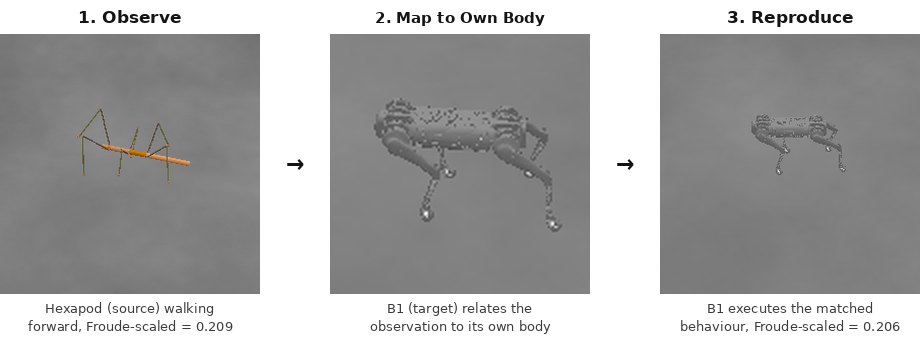
\includegraphics[width=0.85\textwidth]{image/fig_concept_draft.png}
\caption{The transfer this thesis studies: a hexapod's recorded walking (left), observed only as video, is
mapped by the B1 onto its own body through the shared, Froude-scaled coordinate of Section 2.3 (center), and the B1
then executes the matching behavior (right), with no frame pairing, retargeting or kinematic model of either body.}
\label{fig:concept}
\end{figure}

Legged robots are typically controlled by policies learned through reinforcement learning (RL). A persistent and
expensive limitation of this approach is morphology specificity: a policy learned for one body does not
generalize to another. If a robot's legs are lengthened or shortened, its mass distribution changes, or its
skeleton is a different topology altogether, the previously trained policy fails and a new one must be learned
from scratch, a process that can take hours to days of training per body. In contrast, biological organisms share
locomotion principles across vastly different body plans, suggesting that a shared, body-independent
representation of \emph{movement} is possible.

The precise analogy for what this thesis attempts already has a name in psychology: vicarious learning
(Bandura, 1977), the acquisition of a behavior by observing another agent perform it, with no direct instruction,
no first-hand demonstration of the observer's own body doing the task, and no requirement that the observed model
resemble the observer. That is the transfer under test here: a held-out body's controller, with no prior
knowledge of the behavior required of it, is informed by video of a different body's behavior, one it does
not resemble and has never itself performed, with no direct instruction and no kinematic account of either body
supplied to bridge them. The behavior crosses through what is observed, not through anything told to the model
about the bodies involved.

\newpage

Every existing route around this hands the model privileged information about the new body. The
strategies differ mainly in where that information comes from: a CAD or URDF description read directly from the
robot's design files (QWM); a kinematic tree specifying which joint connects to which (graph- and
transformer-based universal controllers); an observation encoder and action decoder fitted per robot from that
robot's own proprioception and foot force (L3P); a task space such as end-effector pose that already means the
same thing on every body in the corpus (LAC-WM); or demonstrations of the same task paired across both bodies
(Demo-JEPA). Each is reasonable, and each assumes access to something about the target body that the motivating
scenario (an animal, a damaged robot, or hardware acquired without published kinematics) does not provide.

One result shows the requirement can be dropped entirely, and it is the starting point for this thesis.
Hu, Chen, and Lipson (2025) learn a task-agnostic visual self-model for a legged robot from a single egocentric
camera and random motor babbling, with no prior knowledge of the robot's morphology, kinematics, or task, and use
it to plan locomotion and even to detect and recover from physical damage. Their claim is that the body
description was never necessary. But their self-model is fitted to \emph{one robot at a time}: each body is
babbled and modeled separately, there is no action representation shared between bodies, and nothing is ever
transferred from one body to another. \textbf{Extending that premise across embodiments is what this thesis
attempts}, and it is the step nobody in this literature has taken.

Why this cannot be answered on bodies that share one skeleton. An earlier phase of this project asked
whether the same idea transfers to legged locomotion using 9 instances of one stick-insect body differing only
in leg-segment lengths. That setting is useful as a controlled first step (Section 1.6, Stage 1) but it cannot, on its own,
establish that \emph{vision} is doing something proprioception could not: several leg-geometry variants share an identical
18-dimensional joint space, so a proprioceptive model could in principle be shared across them too, and vision's
advantage there is convenience, not necessity. Answering the harder question, whether a vision-only latent action
can unify locomotion across bodies where \emph{proprioception has no shared coordinate to begin with}, requires a
second body whose action space is \textbf{disjoint} from the first. This thesis therefore studies 2
robots at once: a simulated 6-legged stick insect (\emph{Medauroidea extradentata}, 18 actuated joints, in
CoppeliaSim) and a Unitree B1 quadruped (12 actuated joints, in MuJoCo). Their joint spaces share no dimension and
no correspondence; a single egocentric camera, by contrast, describes both bodies in the same
$256\times256\times3$ pixel array regardless of what is standing in front of it.

\newpage
The object this thesis learns is not, in the end, a single opaque latent action but a
shared body-motion coordinate: dimensionless forward, lateral, and yaw velocity, the same 3 physical
quantities on both robots, inferred from egocentric video alone, with no morphology label, no kinematic model or
URDF for either body, and no manually defined correspondence between one robot's joints and the other's. Learning
this coordinate is one problem; \emph{using} it to drive an unseen or unfamiliar body is a second, harder problem,
and a substantial part of this thesis is the diagnostic work that separates what the resulting world model can
do (coarse, single-step action-conditioning) from what it cannot yet do reliably (fine-grained action ranking and
multi-step rollout), and the measured mechanism behind that gap.

\textbf{Pursuing that second problem exposed something the prior work never had to confront, and it is the
scientific contribution of this thesis.} Hu et al.\ adopt an egocentric camera for practical reasons: one
onboard sensor, portability, ground texture supplying motion cues, and never compare it against a third-person
view; no method surveyed in Chapter 2 asks whether the viewpoint matters at all. It does, and structurally.
Locomotion is periodic, so an external view of a walking body shows a pose that is itself a function of gait
phase, which makes the command largely readable from the body's own posture. A world model trained on such video
can therefore satisfy its prediction objective by continuing the gait cycle it can already see, without ever
learning what the action does, and this thesis measures that it does. An egocentric view removes
most of that redundancy and restores measurable action-conditioning. The viewpoint from which a locomotion world
model is built is therefore not a free setup choice but a precondition for the model to use its action at all,
which matters here because in cross-embodiment transfer the action is what has to cross.

The significance is twofold. Scientifically, it tests whether a body-independent notion of locomotion behavior
can be learned from visual observation alone, across bodies whose action spaces cannot be reconciled by any
choice of coordinate without a kinematic model, and it produces, along the way, a diagnostic methodology for
telling whether a video world model is \emph{using} an inferred action at all rather than merely being able to
decode it. Practically, if such a coordinate transfers cheaply, it would cut the cost of controlling a new robot
by reusing locomotion behavior already observed on a different body, rather than retraining from zero or
requiring that body's engineering specification.

\noindent\textbf{Why vision rather than each body's own internal sensors.} On flat ground, a single already-known
robot's own joint encoders and an IMU are enough to compute its forward, lateral, and yaw velocity directly, more
simply than reading it from video. That is not in dispute, and it is not the comparison this thesis makes. The
comparison is at the point of transfer: reading a goal from a robot this pipeline has never been given privileged
access to, and driving a second, structurally different robot toward it. Internal sensors require 2 things a truly
unfamiliar robot does not offer, installation and a known kinematic mapping from its joint readings to a shared
coordinate; a camera requires neither, describing any robot in the same pixel array with no per-robot setup at all.
The camera's advantage is therefore specific to the correspondence-free transfer problem this thesis poses, not a
general claim that vision beats proprioception at state estimation on a single known body, and it says nothing yet
about whether an external view's further advantage, seeing terrain and obstacles a body-mounted sensor cannot, holds
here: that is a real extension of this argument, not tested in this thesis.

\newpage
\section{Objectives}
\begin{enumerate}[label=\arabic*.]
\item To learn a shared, dimensionless body-motion coordinate (forward, lateral, and yaw velocity) from egocentric
  simulation video of 2 structurally disjoint legged robots (an 18-DOF hexapod and a 12-DOF quadruped), with no
  morphology label, no kinematic model or URDF for either body, and no frame-level correspondence assumed between
  them, by adapting the Latent Action World Model pipeline (frozen visual encoder $\to$ Inverse Transition Model
  $\to$ Forward Transition Model $\to$ Motion Decoder) from manipulation to locomotion.
\item To demonstrate that this coordinate transfers correspondence-free across the 2 embodiments, in that
  a goal observed on one robot's video can be used to select or drive behavior on the other, and to show
  under which training objective this transfer succeeds and under which it silently fails (a reconstruction-only
  objective is shown to discard the action channel across embodiment families; a discriminative objective is
  required to recover it).
\item To characterize, through closed-loop diagnostic testing, which capability of a video world model's
  action-conditioning is and is not achieved: coarse single-step conditioning, fine-grained action ranking between
  similar candidates, and multi-step rollout, and to identify the measured mechanism responsible for the gap
  between them: gait periodicity, whose severity camera viewpoint determines the visibility of rather than causes,
  and the 2 independent fixes, the camera and the training objective, that restore action use.
\end{enumerate}

\section{Requirements}
Each requirement below is a threshold a stage's experiments must clear before the next stage relies on it, stated
here as what the system must do and measured in Chapter 4 against the full pass criteria of Table~\ref{tab:gates}.
\begin{enumerate}[label=\arabic*.]
\item The decoder must recover a held-out body's command from that body's own frame, not from the identity of the
  nearest training body, verified in Experiment 1.1.
\item The shared body-motion readout, fitted on one embodiment, must transfer to the other with positive $R^2$ in
  both directions, against a mismatched-goal control that must fail where the true comparison succeeds, tested in
  Experiment 2.1a.
\item The forward model's prediction must depend measurably on the true action rather than a null (no-op) action,
  the $\mathrm{null}/\mathrm{real}$ ratio, tested in Experiments 2.4 and 2.3.
\item Closed-loop action selection in the shared coordinate must beat both a random pick and frame-distance scoring,
  tested in Experiment 3.3.
\end{enumerate}
These requirements originate from the 3 objectives of Section 1.2: Requirement 1 is a precondition for
Objective 1's shared coordinate to mean anything; Requirement 2 is Objective 2 stated as a pass/fail test;
Requirements 3 and 4 are Objective 3's action-conditioning question, split into whether the action is used at all
and whether that use is enough to select behavior.

\section{Expected Benefits}
\begin{enumerate}[label=\arabic*.]
\item A demonstration that latent-action world models extend beyond manipulation to legged locomotion across
  bodies whose action spaces are disjoint, not merely differently parameterized instances of one
  topology.
\item Evidence on whether a shared, body-independent locomotion coordinate can be learned \textbf{without}
  privileged morphology information (no CAD/URDF/spec input) or a hand-defined cross-embodiment correspondence,
  using only egocentric video and each body's own auto-logged motion.
\item A reusable diagnostic methodology for distinguishing whether a video world model's inferred action is
  \emph{legible} (decodable by some readout) from whether it is \emph{used} (changes the model's own
  prediction): a distinction this thesis shows does not hold in general, and which prior displacement-based
  evidence for action-sensitivity does not by itself establish.
\item A stated and measured account of what a candidate-scoring deployment strategy requires of an ``unseen''
  robot (a pre-existing policy able to produce the candidate behaviors), why that requirement is circular for
  the problem this thesis poses, and what is required instead (a policy trained to only actuate the robot, not
  to already know how to perform the target behaviors).
\end{enumerate}

\section{Scope of the Research}
\begin{enumerate}[label=\arabic*.]
\item The study is conducted entirely in simulation: the hexapod in CoppeliaSim (Bullet physics engine)
  and the Unitree B1 quadruped in MuJoCo. No physical-robot or sim-to-real deployment is in scope.
\item \textbf{2 stages, 2 different questions.} Stage 1 instantiates one hexapod body as several leg-geometry
  variants sharing an identical 18-dimensional joint space, and establishes that a learned latent
  action can beat a raw-joint-command baseline and transfer to a held-out leg length. That is a controlled result,
  but one that cannot by itself show vision succeeds where proprioception could not, because the 9 variants share
  a joint space proprioception could in principle share too. Stage 2 adds the Unitree B1 quadruped (12 actuated
  joints, MuJoCo), whose action space shares no dimension and no correspondence with the hexapod's, and is the
  setting in which the central claim is tested: a shared body-motion coordinate, inferred from egocentric video
  alone, transfers where no proprioceptive coordinate could be shared at all without first being handed a
  kinematic model of both bodies.
\item The camera is \textbf{egocentric} (mounted on the body, first-person view), not the third-person (allocentric) view used in the project's earlier phase. The reason is the hypothesis developed in Section 2.5: gait phase makes the body's own pose encode the command that produced it, so an allocentric camera, which shows the full external pose, lets a video world model predict the next frame by completing the gait cycle without reading the inferred action. An egocentric camera occludes most of the robot's own body and exposes far less of that redundancy. Whether this holds is tested and not assumed.
\item The behaviors studied are drawn from a curated library of recorded conditions spanning forward, turning,
  and (on the hexapod) sideways locomotion at several speeds, not from an unconstrained action space. A recorded library assumes that the target robot can already produce those
  behaviors; generating the candidates by random motor babbling instead is the route this thesis takes around that
  assumption.
\item The visual encoder (V-JEPA2) is used \textbf{frozen} throughout both stages; training it is out of scope.
\item \textbf{The tested pair is 1 cross-embodiment boundary, not a swept range.} The hexapod (6 legs, 3 joints
  per leg, 18 total) and the B1 (4 legs, 3 joints per leg, 12 total) differ in leg count and total joint count at
  once. Neither leg count alone (for instance 6 legs to 4 legs at matched joints-per-leg) nor joints-per-leg alone
  (for instance 6 legs at 3 joints against 6 legs at 2) is varied independently, and no second quadruped with a
  different gait family (trot against pace against bound) is tested. What this thesis shows is that the coordinate
  crosses this 1 boundary; how far it extends beyond it is not measured.
\end{enumerate}

\noindent\textbf{Explicitly not claimed.}
\begin{itemize}[label=--]
\item Real-robot or animal transfer.
\item Zero-shot cross-embodiment transfer.
\item Reliable multi-step closed-loop control.
\item A scaling law over many pretraining embodiments, in the manner LAC-WM reports.
\item That a camera is the only information this pipeline needs about a new robot.
\item That the tested transfer generalizes beyond the 1 hexapod-to-quadruped boundary studied here to leg
  counts, joint counts, or gait families not tested.
\end{itemize}

\section{Research Procedure}
The project follows a staged, milestone-gated procedure in which each stage's result constrains the design of the
next (each component is validated before the next is built on it):
\begin{enumerate}[label=\arabic*.]
\item \textbf{Stage 1: cross-morphology (prerequisite).} Confirm the pipeline on several leg-geometry variants of one
  hexapod body: that identical commands produce measurably different behavior across leg geometries, that the frozen
  visual encoder carries the behavior signal needed downstream, and that a trained latent action beats a
  raw-joint-command baseline and transfers to a held-out leg length. This stage establishes that the pipeline
  works and that a latent action is better than the alternative; it does not establish that vision succeeds where
  proprioception could not, because all 9 bodies share one joint space (Section 1.1).
\item \textbf{Stage 2: cross-embodiment.} Add the Unitree B1 quadruped, whose 12-dimensional action space shares
  no correspondence with the hexapod's 18. Train a shared visual world-model trunk with per-embodiment decoder
  heads, and test whether a body-motion coordinate learned this way transfers correspondence-free between the 2
  robots, and under which training objective.
\item \textbf{Stage 3: closed loop and controllers.} Build a candidate-scoring loop, in which the world model ranks a
  library of recorded target-robot behaviors against a goal clip, as a test harness for the world model's
  action-selection ability, while explicitly flagging why candidate scoring cannot itself be the final deployment
  mechanism for a unseen robot; and test an imagination-trained policy against the
  same model. Where the loop's behavior does not match what the offline metrics predicted, isolate the mechanism
  through targeted ablations rather than accepting the aggregate closed-loop number as the final word.
\end{enumerate}

\noindent Stage 2 also includes the diagnosis of whether the forward model \emph{uses} the action it is given, and of
the 2 independent fixes (the egocentric camera and the training objective) that restore it.

% ============================================================================
\chapter{LITERATURE REVIEW}

This chapter builds toward a single question. Section 2.1 introduces only the machinery the rest of
the thesis uses. Section 2.2 organizes the cross-embodiment literature on one axis,
\emph{what each method must be told about a robot before it can control it}, because that is the
axis this thesis's claim lives on. Section 2.3 then states what crossing between 2
\emph{structurally different} legged robots additionally requires beyond that axis: a coordinate
that is not joint space. Section 2.4 covers the one result that removes the body-description
requirement entirely, for a single robot, and is the closest precedent to this work. Section 2.5 is
the pivot the rest of the thesis is built on: it asks whether a video world model conditioned on such
a coordinate \emph{uses} it, shows that the literature has not established this for
locomotion, and states the 2-part question, viewpoint and then precision, that the rest of the thesis tests.
Section 2.6 states the resulting gap and the claim of this thesis.

% ============================================================================
\section{Theoretical Background}
This section covers the machinery the argument depends on, and only that. A reader familiar with
world models and self-supervised video representation learning can proceed to Section 2.2.

\subsection{World Models and Learning in Imagination}
A \emph{world model} is a learned model of environment dynamics: given the current state and an
action, it predicts the next state. Once such a model exists, an agent can evaluate or train
behavior by ``imagining'' sequences of hypothetical actions inside it, rather than executing them.
The reference implementation is DreamerV3 (Hafner et al., 2023), which encodes each observation into
a compact latent state and learns the dynamics between latent states, so that the policy is trained
against the model's predictions rather than against the environment (Figure~\ref{fig:dreamer}). A
single agent with one hyperparameter setting mastered more than 150 tasks this way, which
established learned latent dynamics as a general tool.

2 properties matter here. First, the representation the model learns is the object a downstream
policy consumes, so any property that representation has, including independence from the body,
is inherited by everything built on it. Second, and central to this thesis, a world model must answer
``given this state and this action, what happens next?'', which makes its prediction objective an
operational \emph{test} of whether a proposed action representation carries meaningful information
about the change it is supposed to explain. This thesis uses a world model less to imagine long
rollouts than to use that test.

\begin{figure}[ht]
\centering
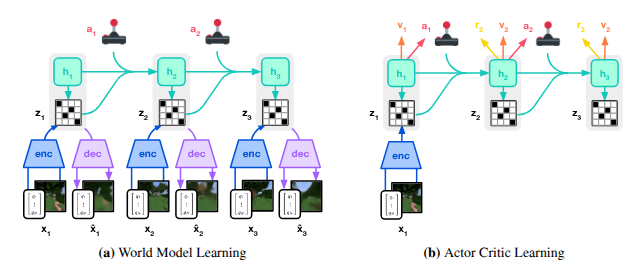
\includegraphics[width=0.75\textwidth]{image/dreamerv3.png}
\caption{The DreamerV3 world model and actor-critic (Hafner et al., 2023). Observations are encoded into a
compact latent state whose evolution a sequence model predicts from actions, and the actor and critic learn on
trajectories imagined inside the model, conditioned on the agent's native action: the body-specific signal this
thesis replaces.}
\label{fig:dreamer}
\end{figure}

The limitation that motivates everything after this is that DreamerV3 and its relatives learn a
separate model per domain and condition on the robot's own motor command. Nothing is shared across
bodies, and the native command is assumed to be the meaningful conditioning signal. When the same
command means something different on a different body, or when 2 bodies have no command in
common at all, that assumption fails.

\subsection{Predicting Representations Rather than Pixels}
To apply a world model to images, one needs features. This work uses V-JEPA~2 (Assran et al., 2025), a
video model trained on roughly one million hours of unlabeled video. Its objective is the
distinguishing feature: instead of reconstructing masked pixels, a Joint-Embedding Predictive
Architecture (JEPA) masks part of the input and predicts the \textbf{representation} of the masked
part. Predicting in representation space frees the model from modeling unpredictable low-level
detail and pushes it toward features that capture how things move and change (Figure~\ref{fig:vjepa2}).

2 aspects are directly relevant. The accompanying V-JEPA~2-AC variant uses the pretrained encoder as
a frozen per-frame image encoder feeding a lightweight downstream predictor, which is the
precedent for how the encoder is used here. And V-JEPA~2 was trained on real-world video
only, so its behavior under a rendering domain gap is uncharacterized, which is why this project
verifies empirically that the frozen features carry the required locomotion signal before relying on
them.

\begin{figure}[ht]
\centering
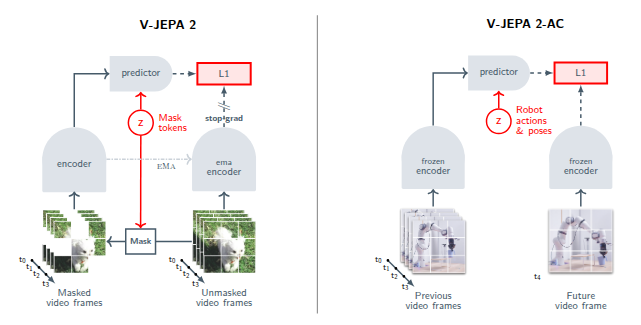
\includegraphics[width=0.65\textwidth]{image/vjepa2.png}
\caption{V-JEPA~2 multistage training (Assran et al., 2025). Left: self-supervised pretraining on
internet-scale video with a mask-prediction objective in representation space. Right: the encoder is frozen and an
action-conditioned predictor is learned on top; this thesis reuses only the frozen encoder.}
\label{fig:vjepa2}
\end{figure}

\subsection{Inverse and Forward Dynamics, and the Latent Action}
2 complementary models recur throughout this literature and form this project's architecture. A
forward dynamics model maps $(s_t, a_t)$ to $\hat{s}_{t+1}$: a world model's transition
predictor is this. An inverse dynamics model maps $(s_t, s_{t+1})$ to $\hat{a}_t$,
answering ``what action caused this transition?'' Neither is any single paper's invention; both are
standard components of learned world models.

The 2 combine into a \emph{latent action}. If the quantity the inverse model recovers is not a
native motor command but an inferred code $z_t$, and the forward model must predict the next state
from the current state plus $z_t$, then the pair jointly learns an action representation: the inverse
model proposes it and the forward model's prediction error tests whether it suffices to explain the
transition. Because $z_t$ is defined by \emph{observed change} rather than by any robot's motor
format, one latent space can in principle describe several bodies, and it can be learned from video
with no action labels at all. CLAM (Liang et al., 2025) introduced \emph{continuous} latent
actions, which suit the smooth, graded control locomotion requires, and LAC-WM (Huang et al., 2026,
next subsection) is the version of the idea this thesis adapts. Whether a latent encodes behavior or
merely copies the next observation is what has to be checked when interpreting it.

\subsection{Latent Action World Models: The Reference Architecture}
LAC-WM (Huang et al., 2026) combines the latent action with a world model to unify one action space
across heterogeneous manipulation embodiments, and is the concrete architecture this project adapts
(Figure~\ref{fig:lacwm}). It has 4 parts: a frozen visual encoder producing $e_t$; an
Inverse Transition Model (ITM) mapping $(e_t, e_{t+1})$ to the latent action $z_t$; a
Forward Transition Model (FTM) predicting $\hat{e}_{t+1}$ from $(e_t, z_t)$; and a
Motion Decoder (MD) mapping $z_t$ back to executable motor commands, which anchors the latent
to real motion so it cannot collapse into a meaningless code. The inverse/forward/decoder skeleton is
the general building block of the preceding subsection rather than LAC-WM's invention; what this
project takes from LAC-WM specifically is its instantiation of that skeleton for cross-embodiment
transfer.

\begin{figure}[ht]
\centering
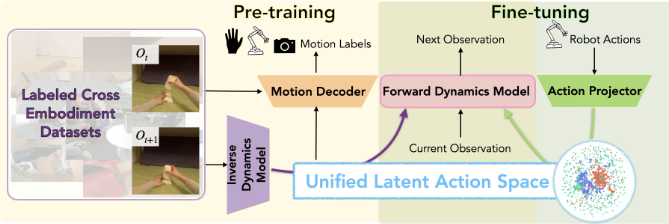
\includegraphics[width=0.8\textwidth]{image/LAC-WM.png}
\caption{LAC-WM (Huang et al., 2026), the architecture this thesis adapts. An inverse model encodes an
observation pair into a unified latent action conditioning a forward model, and a motion decoder maps the latent
back to each embodiment's motor labels; this thesis instantiates the same 2 models on visual embeddings, renamed
Inverse/Forward Transition Models.}
\label{fig:lacwm}
\end{figure}

Because $z_t$ is supervised partly to help reconstruct $e_{t+1}$, the ITM could cheat by copying the
next frame's content into $z_t$ instead of learning an abstract action. LAC-WM prevents this with
\textbf{cross-augmentation}: 2 independent augmentations of the frame pair are encoded, the ITM sees
one while the reconstruction target comes from the other, so a copied pixel-level representation no
longer matches the target. This project inherits the mechanism.

LAC-WM reports that its unified latent transfers across embodiments better than an explicit-action
baseline, and that performance \emph{scales} with embodiment diversity. Its premise, however, is that
the embodiments differ in action format while still decoding into a coordinate that means the same
thing on all of them: end-effector pose. Section 2.3 takes up why that premise does not survive the
move to legged bodies with different leg counts.

\subsection{Measuring What a Representation Contains}
Because the claims here are about what a representation carries, the evaluation uses tools that
measure that. A \textbf{linear probe} trains a simple linear classifier or regressor to
predict a property from a representation; keeping it linear means success reflects the quality of the
representation rather than the cleverness of the readout, so a probe measures the \textbf{presence} of
information in an accessible form. Probes are reported against a chance baseline, under
grouped cross-validation so that success cannot come from memorizing frames of the same clip,
and against a shuffled-label control that must collapse to chance.

A probe measures presence but not dominance: a property can be decodable while contributing almost
nothing to how the representation is organized. The silhouette score and between-class
variance measure that second question. Reporting only one of the 2 gives the wrong answer, and both
are used throughout Chapters 3 and 4. Where the question is not what a representation contains but
whether a \emph{model} uses a quantity, presence-style metrics are insufficient on their own; a
sharper instrument for that question is what Section 2.5 develops.

% ============================================================================
\section{Body Knowledge Required by Existing Methods}
Making 1 controller work across bodies is an active problem, and the strategies differ mainly in
\emph{what they must be told about the new body before they can control it}. Organized this way rather
than by architecture, the literature falls into 4 groups, and a clear pattern holds across all of
them: the body description is always supplied from somewhere.

\subsection{Retraining, with or without a Latent Action}
The traditional strategy is to train a new controller for each body, carrying nothing across. 
Introducing a latent action does not by itself change this. Li et al.\ (2021) plan in a
\emph{learned latent action space} for legged locomotion and demonstrate it on both a hexapod and a
quadruped, but their framework is re-instantiated and trained \emph{separately per robot}: no latent
space or dynamics model is shared or transferred between them. It establishes that latent actions
suit legged control without making the latent space itself the thing that transfers; the cost of
Section 2.1.1 persists even once the action representation is learned rather than native. This is the
reference against which every sample-efficiency claim in this thesis is measured.

\subsection{Explicit Morphology Conditioning}
A second group avoids retraining by being handed a description of the body's structure. QWM
(Danesh et al., 2026) conditions a world model on physical parameters, limb lengths, masses, and torque
limits, read from each robot's CAD/USD description, and generalizes zero-shot to unseen quadruped
morphologies (Figure~\ref{fig:qwm}). It is the strongest cross-morphology transfer result in this
area and the clearest contrast to this thesis: the morphology is \emph{supplied}, not inferred, and
its observation channel is proprioception. QWM also routes what it calls ``unmodeled real-world
residuals'' through a separate dynamic latent, an implicit concession that the design file does not
fully describe the physical body.

\begin{figure}[ht]
\centering
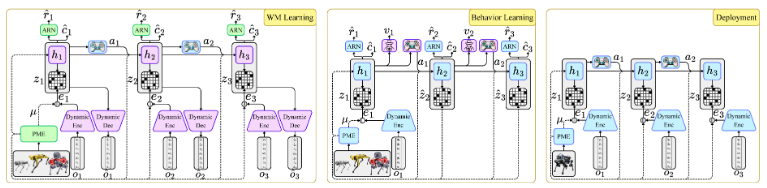
\includegraphics[width=0.85\textwidth]{image/QWM.png}
\caption{QWM (Danesh et al., 2026). A Physical Morphology Encoder embeds each robot's USD design file and
conditions the world model on it; the morphology is supplied from that design file, the privileged input this
thesis removes.}
\label{fig:qwm}
\end{figure}

\newpage
2 related families ask for less than a full design file, but still ask for a structural description.
Graph- and transformer-based controllers such as MetaMorph (Gupta et al., 2022) learn
morphology-agnostic policies over many procedurally varied bodies by representing the body as a graph
of joints; these do not need a CAD file, but they must be handed the \textbf{kinematic tree}, which joint
connects to which. Online system identification instead infers hidden dynamics parameters from a
window of recent interaction, which removes the design file but requires access to the robot's
internal signals and enough new interaction to identify the parameters.

\subsection{Fitted Per-Robot Adapters}
A third group shares a policy \emph{structure} across bodies while still fitting a per-robot
translation layer from that body's own sensing. L3P (Zheng et al., 2025) wraps a shared latent policy
backbone in a per-robot observation encoder and per-robot latent-action decoder, so control transfers
across diverse legged robots (Figure~\ref{fig:l3p}). Its decomposition is a close structural parallel
to this project's shared trunk with body-specific heads. The difference is the channel and the
direction of information: L3P fits its per-robot adapters from that robot's own proprioception and
foot force, with joint ordering and actuator conventions known.

\begin{figure}[ht]
\centering
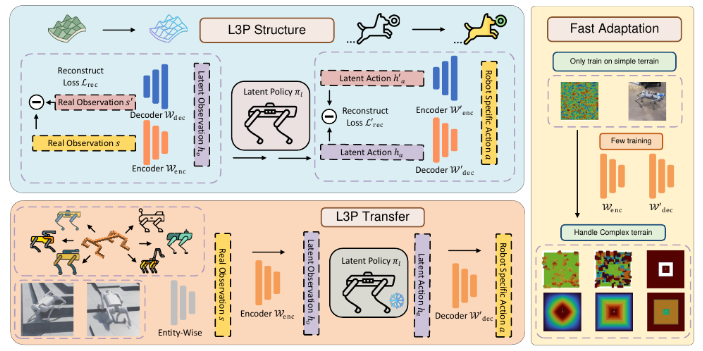
\includegraphics[width=0.6\textwidth]{image/L3P.png}
\caption{L3P (Zheng et al., 2025). A shared latent policy backbone is wrapped by a per-robot observation
encoder and decoder, a structure that parallels this thesis's, but L3P operates on proprioception and must fit an
encoder and decoder per robot.}
\label{fig:l3p}
\end{figure}

\subsection{Alignment Objectives and Paired Demonstrations}
A fourth group obtains the correspondence from data rather than from the body, and it is vision-based.
Demo-JEPA (He et al., 2026) reframes a demonstration as specifying
a future \emph{goal state} rather than actions to copy, and translates source demonstrations into
target-compatible latent goals that the target realizes through its own world model. It requires
neither a shared action space nor action-level retargeting, but the translation is fitted from the
target robot's own interaction experience on trajectories paired with the source: by retargeted
end-effector replay in simulation, and by Global Temporal Cycle Consistency alignment on real data.


\subsection{Synthesis: What Each Method Must Be Told}
Table~\ref{tab:positioning} places these 4 groups on the axes that decide this thesis's claim.
Reading down the ``morphology information'' column, every method obtains the body description from
inside the body, from a design file, or from demonstrations paired on the target. Reading down
``disjoint action spaces'', the methods that do transfer do so across bodies whose action space is
shared by construction, bridged by an adapter fitted with privileged access, or bridged by paired
same-task demonstrations. The vision-based latent-action methods are
demonstrated almost entirely on \textbf{manipulation}, where end-effector pose already provides a
coordinate common to every body in the corpus. Legged locomotion across different leg counts offers
no such coordinate, which Section 2.3 develops.

\begin{table}[H]
\centering
\scriptsize
\setlength{\tabcolsep}{3pt}
\caption{What each method must be told about a robot before it can control it. ``Disjoint action spaces''
asks whether the 2 bodies share no dimension or correspondence without external help; ``transfers across bodies''
asks whether 1 trained model reuses on a new body without retraining from scratch.}
\label{tab:positioning}
\begin{tabularx}{\textwidth}{>{\hsize=1.07\hsize}Y>{\hsize=1.02\hsize}Y>{\hsize=1.07\hsize}Y>{\hsize=1.02\hsize}Y>{\hsize=0.96\hsize\centering\arraybackslash}Y>{\hsize=1.07\hsize\centering\arraybackslash}Y>{\hsize=0.85\hsize}Y}
\toprule
\textbf{Method} & \textbf{Observation} & \textbf{Morphology info.\ from} & \textbf{Action representation} & \textbf{Disjoint action spaces?} & \textbf{Transfers across bodies?} & \textbf{Domain}\\
\midrule
DreamerV3 (Hafner 2023) & state / pixels & retrained per body & native command & n/a & \no\ (per body) & general control\\
Li et al.\ (2021) & proprioception & retrained per body & learned latent action & \yes\ (hex.\ \& quad.) & \no\ (per body) & hexapod, quadruped\\
QWM (Danesh 2026) & proprioception & CAD / USD file & native command & \no\ (quadruped) & \yes\ (zero-shot) & quadruped\\
MetaMorph (Gupta 2022) & proprioception + graph & kinematic tree & native command & \no\ (procedural) & \yes\ (in family) & procedural bodies\\
Online system ID & proprioception & interaction & native command & \no & \yes\ (adapted) & legged / general\\
L3P (Zheng 2025) & proprioception + force & fitted adapter & shared policy latent & \yes\ (adapter) & partial (adapter) & legged\\
LAC-WM (Huang 2026) & vision & from transition & learned latent action & \yes\ (arm, hand, human) & \yes & manipulation\\
Demo-JEPA (2026) & vision & paired target demos & latent goal state & not needed (paired) & \yes\ (with target data) & manipulation\\
Hu et al.\ (2025) & vision (egocentric) & none needed & image-space model & n/a (one robot) & \no\ (per robot) & legged locomotion\\
\textbf{This work} & \textbf{vision (egocentric)} & \textbf{never supplied} & \textbf{shared body-motion coord.} & \yes\ (18 vs.\ 12 DOF) & \textbf{cheap adapt., not zero-shot} & \textbf{legged locomotion}\\
\bottomrule
\end{tabularx}
\end{table}

% ============================================================================
\section{What Cross-Embodiment Locomotion Requires}
Every method in Section 2.2 resolves the correspondence problem by being handed a mapping from
outside: a kinematic tree, a fitted adapter, or paired demonstrations. This section states what a
method that is handed nothing must find instead, before Section 2.4 asks how much of the remaining
requirement, knowledge of the body's own structure, can be dropped as well.

\subsection{A Shared Coordinate That Is Not Joint Space}
An 18-joint hexapod and a 12-joint quadruped have action spaces that share no dimension and no
correspondence. No relabeling creates one: which of the hexapod's 3 joints per leg corresponds to
which of the quadruped's, and what happens to the 2 extra legs, has no physically correct answer.
A method that is handed nothing must instead find a quantity that is \emph{already} the same physical
thing on both bodies and use it as the shared interface.

Task-space foot trajectories are the obvious candidate and are rejected here for 2 independent
reasons. Computing them requires a kinematic model and inverse kinematics for every robot, which is
the cost this work exists to avoid and which fails immediately on a body whose kinematics are unknown.
And empirically, a foot's motion decomposes into the part that is body motion rewritten, adding
nothing not already available, and the gait itself, which is the part that does not
correspond across a 6-legged wave and a 4-legged trot.

What a hexapod and a quadruped share is at the level of the \textbf{body}, not the leg: how
fast the body travels forward, how fast it slides sideways, and how fast it rotates. Those 3
quantities are defined identically on both robots, observable from outside without any kinematic
model, and are what this thesis uses as the shared coordinate.

\subsection{Dynamic Similarity and Froude Scaling}
Comparing those quantities across bodies of different size requires normalizing them. The
dynamic-similarity hypothesis (Alexander and Jayes, 1983) formalizes this for animal gaits:
geometrically similar bodies of different scale move equivalently only when compared at matched
dimensionless speed, the Froude number
\[
Fr = \frac{v^2}{gL},
\]
where $v$ is forward speed, $g$ is gravitational acceleration, and $L$ is a characteristic length (here, leg
length). A normalized forward speed
\[
\tilde{v} = \frac{v}{\sqrt{gL}}
\]
is therefore the scale-free version of ``how fast this body is walking'', and the same reasoning gives
dimensionless lateral speed and yaw rate. This is why the
shared coordinate in this thesis is Froude-scaled rather than expressed in metres per second: without
it, a large quadruped and a small insect walking equivalently would read as different behaviors, and
the coordinate would encode body size rather than behavior.

\newpage
\subsection{The Test Pair, and Why It Is a Valid Dynamic-Similarity Test}
This thesis pairs a simulated stick insect (\emph{Medauroidea extradentata}, source) with a Unitree B1
quadruped (target, MuJoCo). The pair is chosen deliberately, not inherited from prior work: the 2
share no joint correspondence, no leg count, no gait family, and no simulator, so nothing but the
body-level coordinate of Section 2.3.1 can carry information between them, which is what makes the
pair a test of that coordinate rather than a convenient one. The insect side is additionally
chosen because a validated simulation model of the exact species already exists (Larsen et al., 2023)
and its walking is exceptionally well characterized: coordination arises from decentralized local
rules between neighbouring legs rather than a central clock, and at the low,
statically-oriented walking speed used here the gait is a phase-staggered wave rather than a clean
tripod, consistent with both the recordings and the mature controller of Larsen et al. That level of
characterization makes the source body's behavior trustworthy as ground truth.

% ============================================================================
\section{Morphology-Free Self-Modeling}
Section 2.3 defined what a shared interface between 2 disjoint bodies must look like. A separate
question is whether a controller needs to be told anything about a body's structure at all, and one
result removes that requirement entirely: the closest precedent to this thesis.

Hu, Chen, and Lipson (2025) show that a task-agnostic \emph{visual self-model}, a forward model
mapping the current egocentric view and a motor action to the next egocentric view, can be learned
for a legged robot from a single first-person camera and random motor babbling, with no prior
knowledge of the robot's morphology, kinematics, or task.

\begin{figure}[ht]
\centering
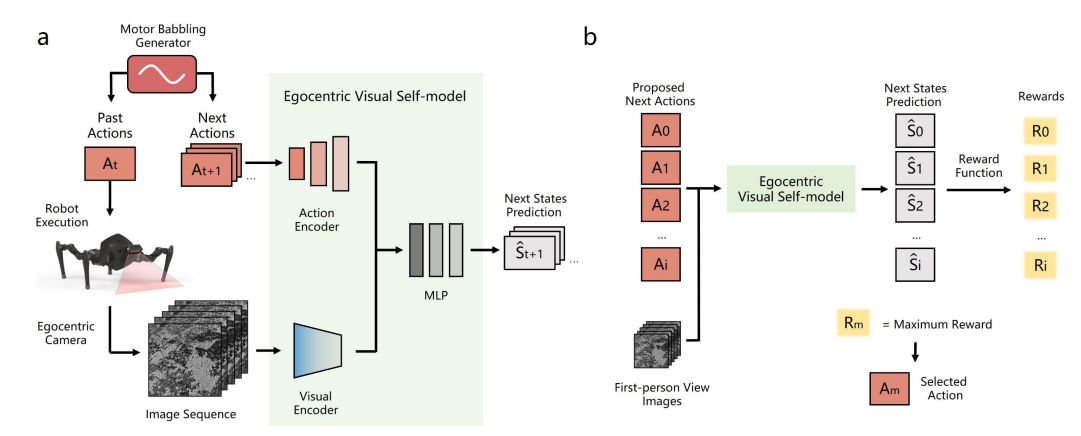
\includegraphics[width=0.85\textwidth]{image/egocentric_vsm.png}
\caption{Egocentric visual self-model (Hu et al., 2025). (a) Motor babbling drives the robot while an
action encoder and a visual encoder feed an MLP that predicts the next egocentric state. (b) Candidate actions are
scored by predicted reward, and the best-scoring one is selected.}
\label{fig:egovsm}
\end{figure}

\newpage
Their argument runs as follows. Legged robots have historically been ``blind'', relying on
proprioception, with vision reserved for high-level planning; the authors challenge the assumption
that vision is too slow and too indirect to model a body's own dynamics. A self-model learned from
vision needs none of the infrastructure its alternatives need: no CAD model or explicit equations,
no IMU, no external optical tracker, no morphology prior, which makes it portable in a way that
matters when a robot must adapt in place. They then widen that claim in stages: basic locomotion
(forward, backward, turning) planned entirely in the visual self-model; robustness to unseen textures
and slippery ground; the same method repeated across several quadrupeds and a humanoid; and finally,
as the capstone, autonomous damage detection and recovery, where the robot notices that its
predictions no longer match what happens, re-babbles, and retrains its self-model, without being told
what broke. Each step widens the same claim: the body description was never necessary.

This thesis adopts that premise directly. 2 things separate the 2 works, and both define what is
left to do.

\textbf{First, the self-model is fitted to one robot at a time.} Each body is babbled and modeled on
its own; the generalization the authors report is that the \emph{method} works when repeated on
different robots, not that one trained model drives a robot it has never interacted with. There is no
shared action representation across bodies, and damage recovery is repair \emph{within} one body's own
model rather than transfer \emph{between} 2. Extending the premise across embodiments is precisely
what this thesis attempts.

Second, the egocentric viewpoint is adopted but never justified against the alternative. The
reasons given are practical: one onboard sensor, portability, and ground texture supplying motion
cues, and no comparison against a third-person view is run. For a self-model of a single body that
is a reasonable and sufficient basis for the choice. Section 2.5 is why, for a \emph{cross-embodiment}
world model, it is not.

% ============================================================================
\section{Action Use in Video World Models}
Everything so far establishes \emph{what} a cross-embodiment method must be given: a shared
coordinate (Section 2.3) that can, following Hu et al.\ (Section 2.4), be inferred with no morphology
description at all. None of it establishes that a world model conditioned on such a coordinate
\emph{depends} on it when predicting. That turns out not to be safe to assume, and it is the
central methodological question this thesis's own diagnostic work is built to answer, in
2 parts: first whether the action is used \emph{at all}, and second, once it is, whether it is used
\emph{precisely enough} to be worth having. This section develops both halves of that question and
shows that neither has been asked in this form before.

\newpage
\subsection{Partial Accounts of Action Neglect}
4 recent results, from 4 different angles, establish that a video world model can appear
action-sensitive by an offline metric while its prediction does not depend on the action,
without any of them measuring how severe this becomes in a periodic domain such as locomotion, or
what causes it (Table~\ref{tab:action-relevance}).

AHA-WAM (Cai et al., 2026) observes, in manipulation world-action modeling, that coupling a world
model's prediction to the same frequency as action execution ``forc[es] the world branch to model
near-term frame variations that are redundant and weakly informative'', and responds by decoupling a
low-frequency video planner from a high-frequency action expert. The redundancy is treated as a design
constraint to work around rather than a phenomenon to explain.

Yeom et al.\ (2026) approach it from the representation side, asking what makes video world model
latents action-relevant. They find that action information is \textbf{legible} in a frozen V-JEPA
encoder's features even though it was never trained with actions ($R^2 \approx 0.40$ frozen, rising to
$0.85$ with a trained inverse-dynamics head), and note separately that static-environment benchmarks
let a model succeed by reading per-frame appearance in place of real temporal reasoning.

UWM-JEPA (Radha and Goktas, 2026) identifies the corresponding pathology in the training objective.
Because the target frame under teacher-forcing is fixed by the trajectory that occurred, a
model can predict it well without its prediction depending on the action it was given. The paper
states the consequence directly: ``action sensitivity itself requires training against counterfactual
rather than teacher-forced targets,'' and proposes counterfactual targets as the remedy.

ActSWM (Gan et al., 2026) names the failure \emph{context collapse}: an autoregressive latent predictor keeps
high similarity to the future states while producing nearly indistinguishable futures under different action
sequences. Its remedy is a transition-separation principle, enforced as a constraint on the latent rollouts:
alternative-action futures should stay distinguishable, and the action behind each local transition should be
recoverable. It is developed and tested on open-world game video (Minecraft planning and cross-game action
recovery), not on locomotion.

\begin{table}[H]
\centering
\footnotesize
\setlength{\tabcolsep}{4pt}
\caption{What each action-relevance result establishes, and what this thesis measures on the same
question.}
\label{tab:action-relevance}
\begin{tabularx}{\textwidth}{>{\hsize=0.47\hsize}Y>{\hsize=1.27\hsize}Y>{\hsize=1.27\hsize}Y}
\toprule
\textbf{Work} & \textbf{What it establishes} & \textbf{What this thesis adds}\\
\midrule
AHA-WAM (2026) & Adjacent frames in manipulation video are ``redundant and weakly informative'' for an
  action-conditioned world model; responds architecturally. & Asks \emph{why} the redundancy arises in
  legged locomotion, and whether it is a property of the viewpoint rather than of the frame rate.\\
Yeom et al.\ (2026) & Action information is \emph{legible} in a frozen video encoder not built for the
  purpose ($R^2\!\approx\!0.40$ frozen, $0.85$ with a head). & Distinguishes legibility from use: a
  model can make the action more readable in its output while depending on it less.\\
UWM-JEPA (2026) & Teacher-forced targets let a model satisfy its objective without depending on the
  action; proposes counterfactual targets. & Examines a domain where the action-independent prediction
  is already near the achievable ceiling, so the proposed remedy has little remaining gap to close.\\
ActSWM (2026) & Names context collapse (rollouts that stay close to the future while ignoring which actions were
  taken) and enforces separation between alternative-action rollouts. & Applies a separation term and a frozen
  action readout to a legged-locomotion world model, and measures how much of the collapse they remove.\\
\bottomrule
\end{tabularx}
\end{table}

\subsection{The Unexamined Variable: Camera Viewpoint}
None of the 4 above asks the question this thesis is forced to confront: \textbf{how
severe the redundancy becomes when the observation is periodic, and whether the camera viewpoint
determines it.} Locomotion is periodic by construction, and an external, third-person view of a
walking body shows a pose that is itself a function of gait phase: the body's own posture can stand
in for the command that produced it. Whether that makes the action redundant or
an egocentric view removes the redundancy, is tested in this thesis.
It is also the question Hu et al.\ (Section 2.4) never had to ask, because a self-model of one's own
body has no allocentric alternative to compare against.

\subsection{Legibility, Use and Precision of the Action}
An inferred action is legible does not show a world model \emph{uses} it: a model's output can become \emph{more} legible in the way such a
metric rewards while its actual dependence on the action falls. None of the 4 results in Section
2.5.1, or any other method reviewed in this chapter, treats ``the model uses the action at all,''
``the model uses it precisely enough to rank similar candidates,'' and ``the model uses it reliably
over many steps of rollout'' as separate claims requiring separate evidence. Each is evaluated, at
most, on whichever single one of these its own benchmark happens to test, and success on one is
routinely read as evidence for the others. That conflation, treating action-sensitivity as a single
property rather than as (at least) 3, is itself a gap in how this literature evaluates
action-conditioned video world models, independent of any particular domain or method.

\newpage
% ============================================================================
\section{Research Gap and the Claim of This Thesis}
Section 2.2 established that every cross-embodiment method must be told something about the new body:
a design file, a kinematic tree, a fitted adapter, or demonstrations paired on the target. Section 2.3
established what a method that is told nothing must find instead: a shared coordinate that is not
joint space, Froude-scaled so it encodes behavior rather than body size. Section 2.4 established that
the remaining requirement, knowledge of a body's own structure, can also be dropped entirely, for a
single robot, and that nobody has extended that to a second. Section 2.5 established that even once
both of those are granted, a further and largely unexamined question remains: whether the resulting
world model uses the coordinate it is given at all, uses it precisely enough to rank similar
candidates, and uses it reliably over more than one step: 3 separate claims the literature does
not treat as separate, and the influence of camera viewpoint on the first of these is
unexamined altogether.

The gap is the conjunction, and no surveyed method occupies it: \textbf{vision-only observation, no
kinematic model or design file for either body, disjoint action spaces (18 against 12
joints, 6 legs against 4), and evaluation through closed-loop control rather than an offline
number alone.}

\noindent\textbf{The claim this thesis makes.} A behavior recorded on one robot can drive a
structurally different robot from egocentric video alone, with no URDF, no kinematic model, and no
demonstrations of the target body, through a Froude-scaled body-motion coordinate; and the viewpoint
from which that world model is built is not a free choice, because in periodic locomotion an external
view lets the body's own pose stand in for the command and the world model never learns to use the
action.

\noindent What is deliberately not claimed is set out in Section 1.5 and repeated here in one
line: not zero-shot transfer, not reliable long-horizon closed-loop control, not a scaling law over
many embodiments, and not that a camera is currently the only thing this pipeline needs about a new
robot.

\noindent\textbf{Why simulation.} Answering this requires 2 bodies whose action spaces are verifiably disjoint, driven under known conditions, with
exact body pose and contact logged, and the ability to hold the camera and the rendering fixed while
only the viewpoint changes. Only simulation provides that, and it is what makes the viewpoint
comparison a controlled measurement rather than an observation. Real-robot transfer is
out of scope (Section 1.5); the contribution is the controlled demonstration of what does and does not
cross, and why.

\newpage
\noindent\textbf{On the observation modality.} Vision is chosen over
proprioception for different reasons in the 2 stages of this work. Across several leg-geometry
variants of one hexapod (Stage 1), the 9 bodies share an 18-dimensional joint space, so
proprioception could in principle be shared too and vision is the harder demonstration rather than a
necessity. Across the hexapod and the quadruped (Stage 2), there is no proprioceptive coordinate to
share without first constructing a joint correspondence from outside, the privileged
information this thesis withholds, while one camera describes both bodies in the same pixel array.
The strongest version of the argument is not that proprioception is incapable: morphology-agnostic
proprioceptive control exists, treating joints as a token set over the kinematic graph. It is that
those methods must be handed the graph, and a camera has to be handed nothing. That distinction also
decides which bodies the approach could ever reach: animals, robots whose configuration has diverged
from their documentation, and hardware acquired without published kinematics are all cases where an
external view is the only channel left.

\chapter{RESEARCH METHODOLOGY}

\section{System Overview}
The system comprises 5 learned/parameterized components on top of a fixed perceptual front-end, trained
end-to-end except for the frozen encoder, and shared across both embodiments with 2 exceptions noted below:

\begin{figure}[H]
\centering
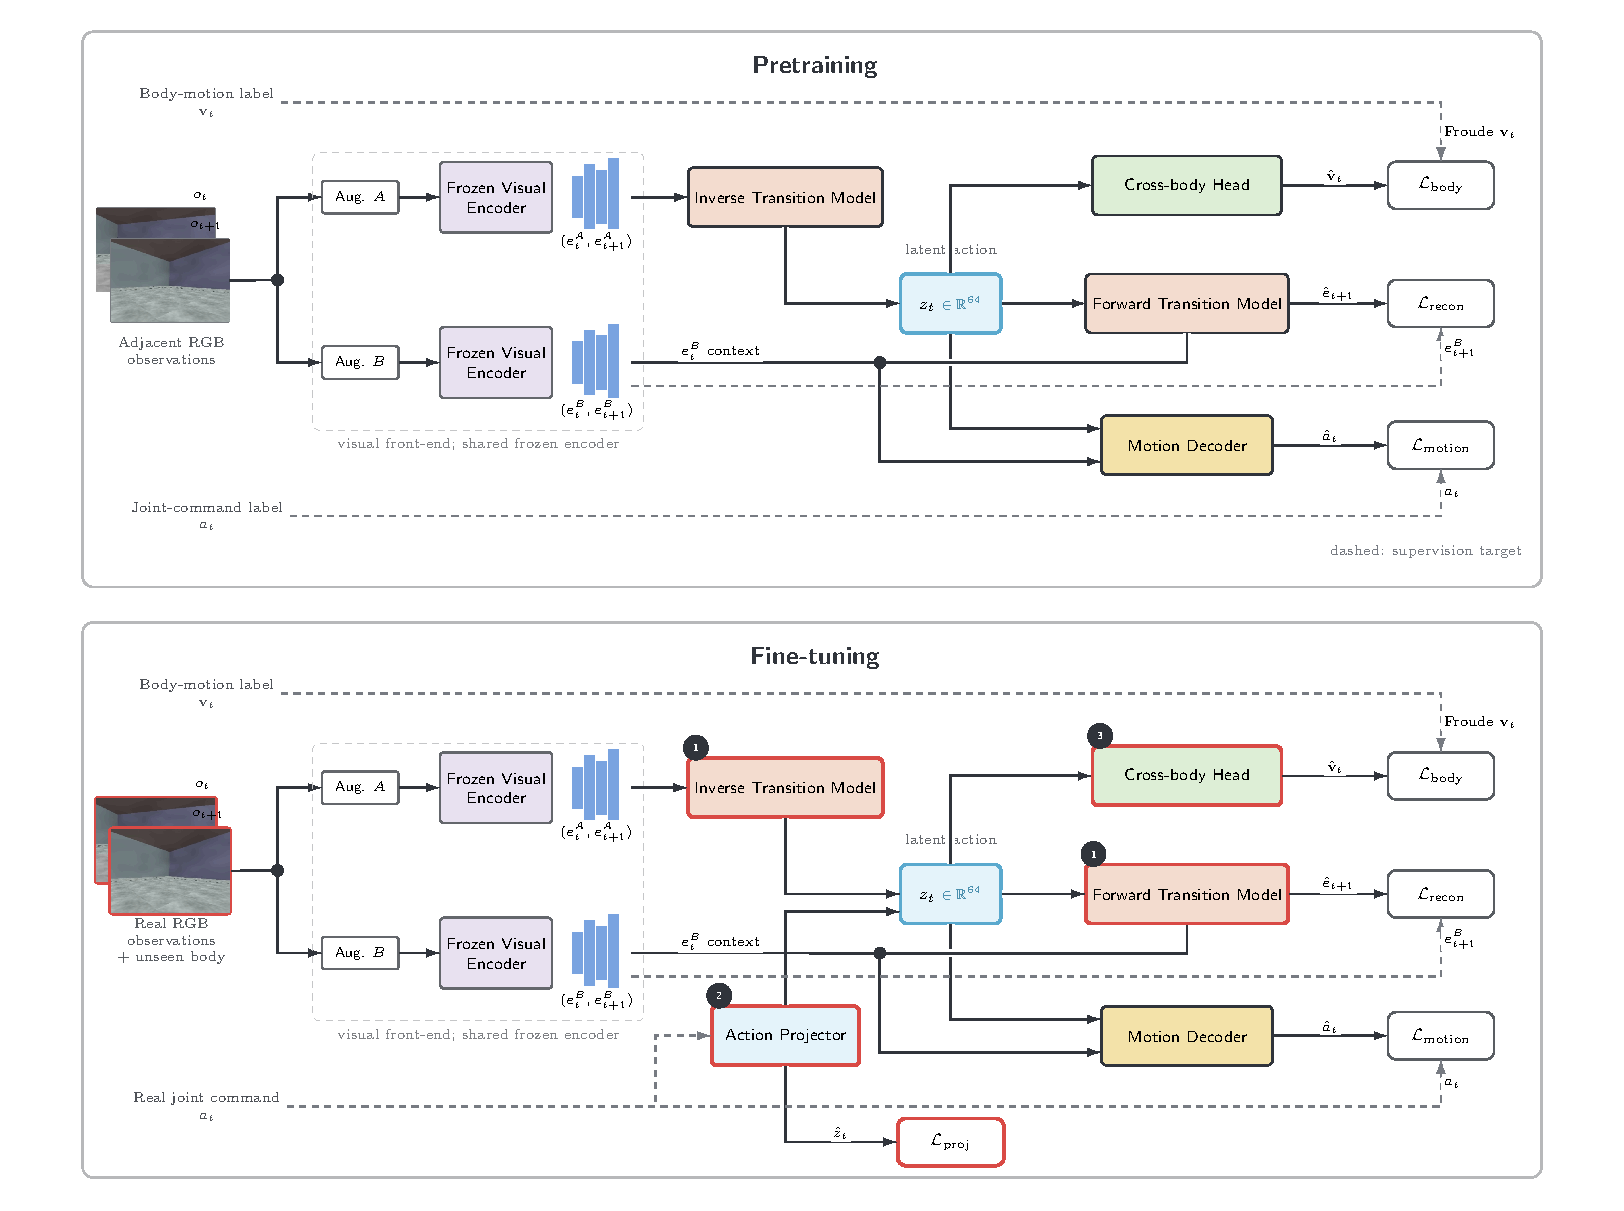
\includegraphics[width=\textwidth,trim=38pt 14pt 38pt 14pt,clip]{image/pipeline.pdf}
\caption{Pretraining (top) and fine-tuning on a new body (bottom). A frozen V-JEPA 2 encoder maps each RGB frame to an
embedding $e_t$; the Inverse Transition Model infers the latent action $z_t$ from $(e_t, e_{t+1})$; the Forward
Transition Model predicts $\hat{e}_{t+1}$ from $(e_t, z_t)$ (loss $\mathcal{L}_{\text{recon}}$); the Motion Decoder maps
$z_t$ back to a body-specific joint command $\hat{a}_t$ (loss $\mathcal{L}_{\text{motion}}$) through a per-embodiment
head; and the Cross-Body Head maps $z_t$ to the shared body-motion label (loss $\mathcal{L}_{\text{body}}$), which is what
carries the cross-embodiment claim. Fine-tuning adds the Action Projector; the numbered circles mark the adaptation step
in which each module is trained (Section 3.4.5).}
\label{fig:pipeline}
\end{figure}

\begin{table}[H]
\centering
\footnotesize
\setlength{\tabcolsep}{4pt}
\caption{Input/output specification of each block in the pipeline. Per-embodiment blocks give hexapod / B1 shapes.}
\label{tab:io}
\begin{tabularx}{\textwidth}{>{\hsize=0.91\hsize}Y>{\hsize=1.12\hsize}Y>{\hsize=1.12\hsize}Y>{\hsize=0.84\hsize}Y}
\toprule
\textbf{Block} & \textbf{Input} & \textbf{Output} & \textbf{Trained?}\\
\midrule
V-JEPA2 encoder & RGB frame, $256\times256\times3$ (uint8) & $e_t \in \mathbb{R}^{256\times1408}$ patch tokens & No (frozen)\\
Inverse Transition Model & $[e_t, e_{t+1}]$ (512 tokens) & $z_t \in \mathbb{R}^{64}$ (latent action) & Yes\\
Forward Transition Model & $[e_t, z_t]$ & $\hat{e}_{t+1} \in \mathbb{R}^{1408}$ & Yes\\
Motion Decoder (per-embodiment head) & ($e_t$ as context, $z_t$ as query) & $\hat{a}_t \in \mathbb{R}^{18}$ /
  $\mathbb{R}^{12}$ (joint targets, rad) & Yes\\
Cross-body head (shared, frame-blind) & $z_t$ only & $\hat{v}_t \in \mathbb{R}^3$ (forward, lateral, yaw;
  Froude-scaled, dimensionless) & Yes\\
Action projector (per-embodiment) & $a_t$ (control time, no future frame available) & $z_t \in \mathbb{R}^{64}$ & Yes\\
\bottomrule
\end{tabularx}
\end{table}

The training loss is
\[
\mathcal{L} = \lambda_{\text{recon}}\,\mathcal{L}_{\text{recon}} + \lambda_{\text{motion}}\,\mathcal{L}_{\text{motion}}
  + \lambda_{\text{body}}\,\mathcal{L}_{\text{body}},
\]
with the 3 terms
\begin{gather}
\mathcal{L}_{\text{recon}} = \lVert \hat{e}_{t+1} - e_{t+1} \rVert^2, \label{eq:recon}\\
\mathcal{L}_{\text{motion}} = \lVert \hat{a}_t - a_t \rVert^2, \label{eq:motion}\\
\mathcal{L}_{\text{body}} = \lVert \hat{v}_t - v_t \rVert^2, \label{eq:body}
\end{gather}
and $(\lambda_{\text{recon}}, \lambda_{\text{motion}}, \lambda_{\text{body}}) = (1.0, 1.0, 0.5)$ in the base objective. Equation~\eqref{eq:recon} is computed in embedding space, so no pixel decoder is
required; Equation~\eqref{eq:motion} is supervised through the per-embodiment head; Equation~\eqref{eq:body} is
supervised through the \emph{shared} head, the only term that asks the same $z_t$ to decode the same way on both
robots (Section 3.4.4). This weighting, every other hyperparameter, and the full parameter count of every module
are given in full in Appendix A.

The Stage 2 and Stage 3 checkpoint adds 3 terms to the base objective, 2 that separate and ground and 1 that anchors: a hinge with weight $\lambda_{\text{hinge}}=0.5$, a frozen action readout with $\lambda_{\text{readout}}=1.0$, and a 2-step rollout loss with $\lambda_{\text{rollout}}=1.0$, with hinge horizon $K=2$ and margin $m=0.1$.

\newpage
\noindent (1) Hinge loss: separate the real-action rollout from the null-action rollout (ActSWM). Both rollouts
start from the same frame and run through the Forward Transition Model for $K$ steps; only the latent differs:
\begin{gather}
z = \mathrm{ITM}(e_t,\, e_{t+1}), \qquad z_{\varnothing} = \mathrm{ITM}(e_t,\, e_t) \\
\hat e^{\,\mathrm{real}}_{t+k} = \mathrm{FTM}\big(\hat e^{\,\mathrm{real}}_{t+k-1},\, z\big), \qquad
\hat e^{\,\mathrm{null}}_{t+k} = \mathrm{FTM}\big(\hat e^{\,\mathrm{null}}_{t+k-1},\, z_{\varnothing}\big), \qquad
\hat e^{\,\mathrm{real}}_{t} = \hat e^{\,\mathrm{null}}_{t} = e_t \\
\ell_k = \max\!\Big(0,\; \cos\!\big(\hat e^{\,\mathrm{real}}_{t+k},\, \hat e^{\,\mathrm{null}}_{t+k}\big) - (1 - m)\Big) \\
\mathcal{L}_{\text{hinge}} = \frac{1}{K}\sum_{k=1}^{K} \ell_k
\end{gather}
\begin{itemize}[label=--]
\item The term is one-sided: once the 2 rollouts are $m$ apart in cosine distance it gives no gradient. It says
  ``different'', never ``correct''.
\item $m = 0.1$, not the paper's 0.3: at 0.3 the term overshoots, switches itself off and collapses (separation
  $0.019 \to 0.137 \to 0.496 \to 0.008$, gradient down to $6\times10^{-5}$).
\item $K = 2$, not the paper's 12 (nor the implementation's default 3): it is set to the depth the anchor in (3) covers.
\item The null is $\mathrm{ITM}(e_t, e_t)$, not a standing-still action: pretraining has no action projector, and a
  hinge built on the projected standing action sends exactly zero gradient into $z$.
\end{itemize}

\noindent (2) Frozen action readout: the rolled-forward prediction must still carry the action (ActSWM). A
randomly initialized, never-trained 2-layer MLP $R$ (hidden width 512, GELU) reads the start frame and the last step of
the real rollout and must recover the command:
\begin{gather}
\hat a_t = R\big(\bar e_t,\; \bar{\hat e}^{\,\mathrm{real}}_{t+K}\big), \\
\mathcal{L}_{\text{readout}} = \mathrm{MSE}\big(\hat a_t,\; a_t\big),
\end{gather}
where $\bar e$ is the mean over tokens and $a_t$ is the recorded command window.
\begin{itemize}[label=--]
\item $R$ is frozen and random on purpose: a readout that learns could move the boundary it is scored against (an
  earlier contrastive repair did that). A fixed map cannot, so the only way to lower the loss is to make the
  predicted transition itself carry the action. Gradient flows through $\hat e^{\,\mathrm{real}}_{t+K}$ into the FTM and,
  through $z$, into the ITM; the readout's own weights never change.
\item Nothing downstream uses its output; it exists to route gradient into the forward model.
\end{itemize}

\newpage
\noindent (3) Rollout loss: a 2-step auto-regressive consistency loss that anchors the prediction
(Demo-JEPA). The FTM's own step-1 output is fed back in as the input of step 2, and step 2 is scored against the true
$e_{t+2}$:
\begin{gather}
z_2 = \mathrm{ITM}(e_{t+1},\, e_{t+2}) \quad \text{(real frames only)} \\
\hat e_{t+1} = \mathrm{FTM}(e_t,\, z), \qquad \hat e_{t+2} = \mathrm{FTM}(\hat e_{t+1},\, z_2) \\
\mathcal{L}_{\text{rollout}} = \mathrm{MSE}\big(\hat e_{t+2},\; e_{t+2}\big)
\end{gather}
\begin{itemize}[label=--]
\item $z_2$ never comes from $\hat e_{t+1}$, so an inaccurate step 1 cannot relabel what the second action means; only
  the FTM's input is auto-regressive.
\item It needs a third frame per sample.
\item The anchor covers the same 2 steps as the hinge horizon ($K=2$).
\end{itemize}

\noindent The full objective is
\begin{equation}
\mathcal{L} = \mathcal{L}_{\text{base}} + \lambda_{\text{hinge}}\mathcal{L}_{\text{hinge}}
+ \lambda_{\text{readout}}\mathcal{L}_{\text{readout}} + \lambda_{\text{rollout}}\mathcal{L}_{\text{rollout}},
\end{equation}
where $\mathcal{L}_{\text{base}}$ is the base objective above (next-frame reconstruction, command decoder and Cross-Body Head).

\textbf{Cross-augmentation} is applied throughout: 2 independent augmentations of each frame pair are encoded,
one feeding the ITM and the other the FTM's reconstruction target, which prevents the ITM from smuggling raw
future-frame content into $z_t$ as a shortcut. One sampled augmentation is applied identically to \emph{both}
frames of a pair, so the transition itself carries no augmentation difference; a second, independently sampled
augmentation gives the reconstruction target its own view. Each augmentation is a random square crop (side length
uniform in $[0.85, 1.0]\times$ the frame's shorter side, resized back to $256\times256$) combined with an
independent random brightness shift ($\pm0.2$) and contrast scale ($\times[0.8, 1.2]$). A horizontal flip is
deliberately excluded: mirroring the image would swap the robot's left and right legs while the supervised joint
command keeps its original leg ordering, which would make the Motion Decoder's target inconsistent with what the
frame shows.

\section{Simulation Environment and Embodiments}

\subsection{Simulators and Models}
2 simulators host the 2 embodiments. The \textbf{hexapod} is the \emph{Medauroidea extradentata} model (6
legs, 3 actuated joints each: ThC/CTr/FTi), with an 18-dimensional joint-position-target action space,
simulated in CoppeliaSim v4.10 (Bullet 2.78 engine, 20~Hz timestep). The CoppeliaSim model itself is adapted from an existing lab asset built for a separate,
unpublished project of the same lab; The Unitree B1 is a quadruped with a 12-dimensional joint-position-target action space, simulated in MuJoCo.
The 2 share no simulator, no joint count, no joint convention, and no gait family (Section 2.3.3); nothing but
the shared body-motion coordinate of Section 3.4.4 is available to connect them.

\begin{figure}[H]
\centering
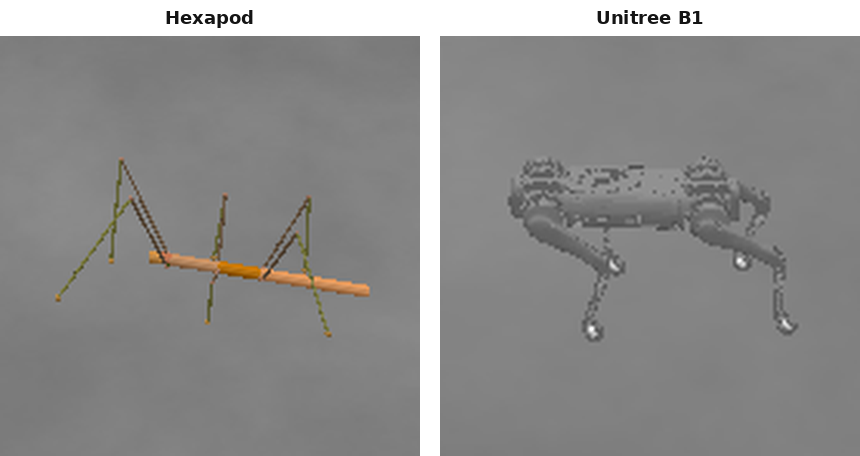
\includegraphics[width=0.65\textwidth]{image/fig_body_closeup_draft.png}
\caption{Close-up renders of both simulated bodies. The hexapod's 6 legs (18 joints) and the B1's 4 legs (12
joints) share no joint count, convention or topology, the premise the shared coordinate of Section 3.4.4 works
around.}
\label{fig:body-closeup}
\end{figure}


\subsection{Embodiments and Leg-Geometry Variants}
The hexapod is additionally instantiated as multiple leg-geometry variants, scaling the coxa, femur, and
tibia segments of all 6 legs \emph{independently} (each segment's own factor, verified numerically per leg by
measured foot-reach) rather than by one uniform leg-length factor. Morphology is therefore a 3-dimensional
volume of possible bodies, not points along a single long/medium/short axis, and a held-out body can be a
combination of segment scales no training body used. Stage 1's main dataset is \textbf{9 such bodies}
(30 clips each, 270 clips). 2 of them, both with the femur scaled 0.6 and the tibia 1.0,
stumble and are dropped. 5 bodies train; the body with segment scales (0.8, 0.9, 0.9) is held out entirely and lies inside
the training bodies' convex hull, and in a second run the body with scales (0.6, 0.6, 0.6) is held out and lies outside it. This \textbf{multi-body} substrate is \textbf{Stage 1}: a controlled,
same-topology testbed used to validate the pipeline and the value of a latent action over a raw command before the
harder, disjoint-action-space claim is attempted. \textbf{Stage 2} pairs the hexapod (base geometry) with the Unitree B1 and
is the setting of every later experiment.

\subsection{Egocentric Observation Capture}
The camera is mounted on the body (first-person, egocentric) for both embodiments, not the third-person
(allocentric) view used in this project's earlier phase. This is a design choice with a reason: Section 2.5.2
argues that an allocentric view of a periodic gait lets the body's own pose stand in for the command, which would make
it impossible to show that a world model uses the action at all. The
floor uses a matte, mildly-textured, non-repeating surface (a controlled choice: both a stark checkerboard and a
blank surface were found to corrupt the visual features). Camera intrinsics and mounting pose are held fixed
within each embodiment so that only the viewpoint category (ego/allo), not incidental camera differences,
distinguishes the 2 views.

\begin{figure}[H]
\centering
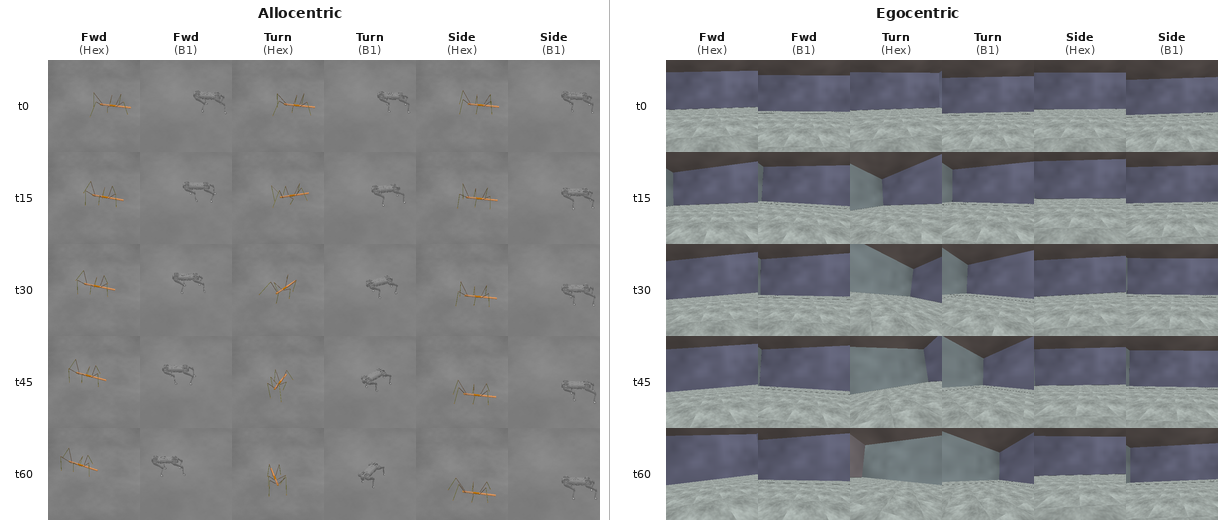
\includegraphics[width=0.85\textwidth]{image/fig_filmstrip_combined_draft.png}
\caption{Representative clips from the curated behavior library (Section 3.6.5), allocentric (left) and
egocentric (right). Each column pairs a hexapod condition with its Froude-matched B1 condition (forward, turn and
strafe), matched as in Section 3.4.4.
Every pair is the strongest available condition on each behavior axis, not the weakest chosen for visual
convenience, and both members of a pair are within 24\% of each other on the dimensionless quantity the shared
cross-body head is trained against.}
\label{fig:filmstrip}
\end{figure}

The 2 viewpoints capture visibly different motion regimes even before any model sees them. Mean frame-to-frame
pixel difference (grayscale, matched forward condition above) is roughly 9 times larger egocentrically than
allocentrically on both bodies (hexapod 6.10 against 0.68, B1 4.16 against 0.56), and the egocentric peak-to-mean
ratio (1.60--1.65) is higher than the allocentric one (1.23--1.25), consistent with a periodic, gait-locked camera
oscillation rather than incidental noise. Figure~\ref{fig:motion-energy} plots this directly, and
Figure~\ref{fig:ego-overlay} shows what it looks like in the frames themselves: 9 real egocentric frames per
body, sampled evenly across the clip, overlaid by taking the per-pixel maximum of each frame's edge map after
tinting it by its position in time (early frames blue, late frames red). Where the camera holds a steady pose
across the clip, edges from different times land on the same pixels and the overlay reads as a tight, single-
colored trace; where it does not, the same physical edge appears at different pixel locations at different times
and the overlay fans out into visibly separated colors. The hexapod's overlay fans out considerably more than the
B1's, which is the direct visual counterpart of its larger, and less steady, frame-to-frame pixel difference.

\begin{figure}[H]
\centering
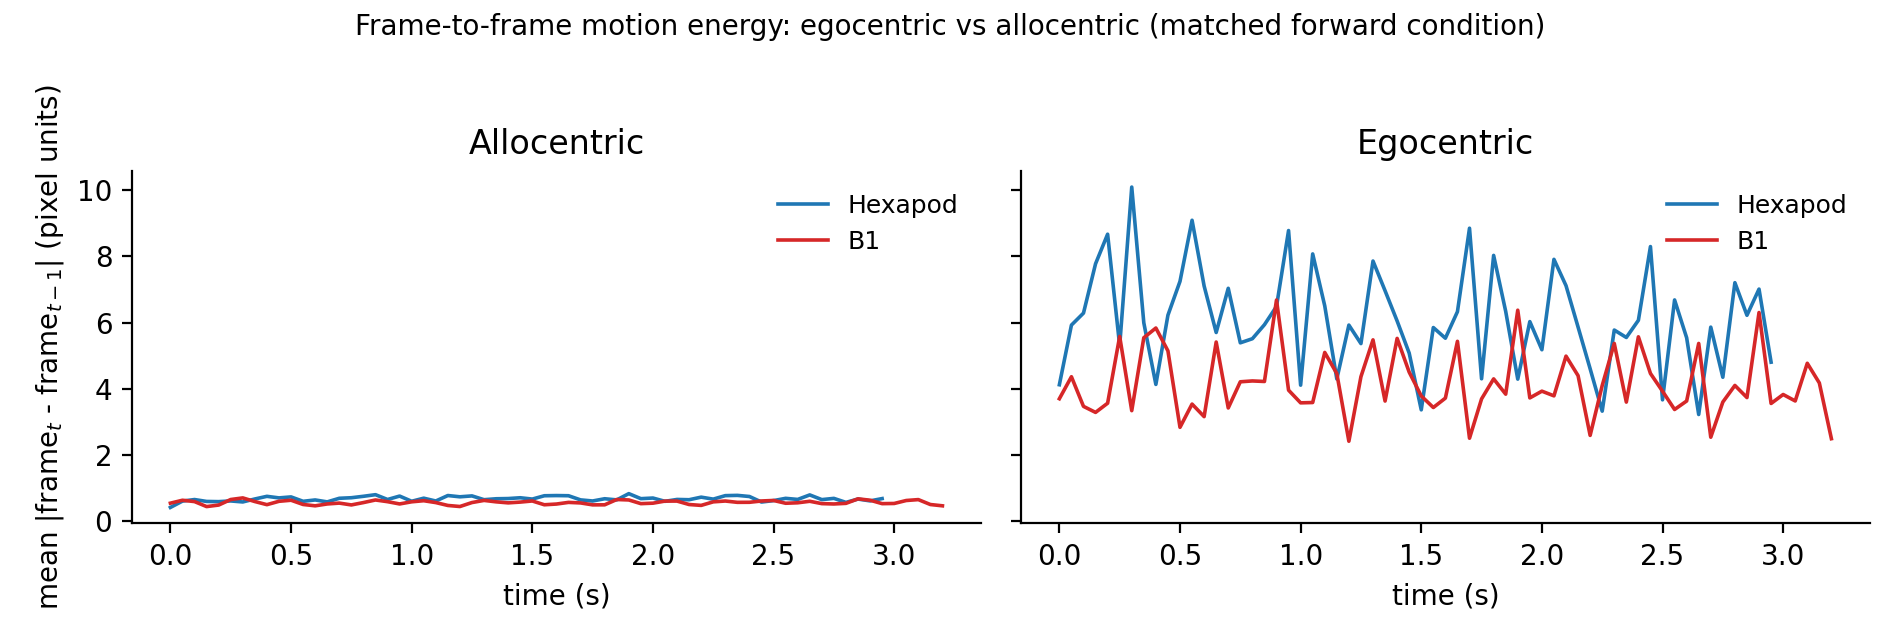
\includegraphics[width=0.85\textwidth]{image/fig_motion_energy_draft.png}
\caption{Mean absolute frame-to-frame pixel difference over time, allocentric (left) and egocentric (right), same
matched forward condition as Figure~\ref{fig:filmstrip} (the fastest speed of each body).
Shared $y$-axis across both panels.}
\label{fig:motion-energy}
\end{figure}

\begin{figure}[H]
\centering
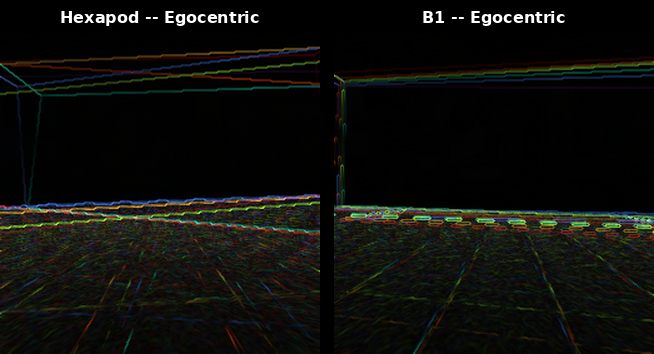
\includegraphics[width=0.6\textwidth]{image/fig_ego_overlay_draft.png}
\caption{Time-coded overlay of 9 egocentric frames from the clips of Figure~\ref{fig:motion-energy} (blue
earliest, red latest). Tight, single-colored edges mean a steady camera pose; spread, multi-colored edges mean the
pose is changing.}
\label{fig:ego-overlay}
\end{figure}

\section{Visual Encoder (Frozen V-JEPA2)}
The encoder is V-JEPA 2 ViT-g/16 (${\sim}1$B parameters), used frozen for both
embodiments. Because this checkpoint is natively a 64-frame \emph{video} encoder with 2-frame tubelets, feeding a
real clip would let each frame attend to other timesteps and contaminate its embedding. To obtain an independent
per-frame embedding, each frame is duplicated into the minimal 2-frame tubelet and encoded alone,
yielding 256 patch tokens of dimension 1408 per frame. This usage has direct precedent in V-JEPA~2-AC.

\section{Latent Action Model}
The 2 learned transition models below are instances of the inverse and forward dynamics models described in
Section 2.1.3: the ITM infers the latent action from a state transition, and the FTM predicts the next state from
the current state and that latent. This project refers to them as Transition Models rather than
\emph{dynamics} models deliberately: the name states what the module computes (a mapping over embedding
transitions) without implying that it estimates the body's physical dynamics, which it does not.

\subsection{Inverse Transition Model (ITM)}
Attention-based (causal self-attention blocks with a learned query token) mapping the pair $[e_t, e_{t+1}]$ to the
latent action $z_t \in \mathbb{R}^{64}$. The causal structure frames $z_t$ as ``what happened between $t$ and
$t+1$.'' This is the inverse dynamics model of Section 2.1.3, computing $z_t$ from a transition instead of a
native action, and it is shared, unmodified, across both embodiments: there is exactly one ITM.

\subsection{Forward Transition Model (FTM)}
Attention-based, predicting the next visual embedding $\hat{e}_{t+1}$ from $[e_t, z_t]$; supervised by
$\mathcal{L}_{\text{recon}}$ in embedding space. Like the ITM, there is one FTM shared across both embodiments; its
dependence on $z_t$ is the property the evaluation of Section 3.6 tests.

\subsection{Motion Decoder (MD)}
Cross-attention with $z_t$ as query over the current visual context, producing $\hat{a}_t$ through a
\textbf{per-embodiment} head; supervised by $\mathcal{L}_{\text{motion}}$ against each body's own auto-logged
joint command. Its role during pretraining is to anchor $z_t$ to real motion so the latent cannot collapse into a
trivial identity. Because its heads are per-embodiment and its targets (18-D and 12-D joint commands) have no
correspondence with each other, $\mathcal{L}_{\text{motion}}$ alone cannot force $z_t$ to mean the same thing on
both bodies: nothing prevents the shared trunk from partitioning by embodiment underneath 2 separately-fitted
heads. That is the job of the next module.

\subsection{Cross-Body Head: The Cross-Embodiment Claim}
A single head, shared by both embodiments and given no access to the frame, maps $z_t$ alone to the Froude-scaled
body-motion coordinate of Section 2.3 (forward, lateral, yaw), supervised by $\mathcal{L}_{\text{body}}$. Being
frame-blind is deliberate: a head that could see the frame could identify which robot it is looking at and learn
a de facto per-embodiment mapping underneath a nominally shared head, which an earlier ablation of this design
confirmed happens when the frame is made available. Being the \emph{only} term supervised through a head shared,
unmodified, across both robots is what makes $\mathcal{L}_{\text{body}}$, not $\mathcal{L}_{\text{motion}}$, not
$\mathcal{L}_{\text{recon}}$, the term that can force $z_t$ to carry a cross-embodiment meaning.

\subsection{Action Projector}
A small per-embodiment MLP mapping a body's own logged command $a_t$ to a latent $z_t$, used only where the ITM's
required future frame $e_{t+1}$ is unavailable: at control time, when only the current observation exists. It
is fitted to reproduce, from the command alone, the latent the ITM would have inferred from the corresponding
transition, and it is what lets a recorded command be converted into a query against the shared latent space
during closed-loop evaluation.

\noindent\textbf{Adaptation to a new body, in 3 steps.} A body that was not in pretraining is adapted from the
hexapod-only pretrain in 3 steps; ``Stage'' is reserved for the data and experiment stages of this thesis, and the
steps are numbered separately (Figure~\ref{fig:pipeline}). \textbf{Step 1} fine-tunes only the ITM and FTM on a handful of
the new body's clips. \textbf{Step 2} fits the Action Projector of this section against the frozen ITM. \textbf{Step 3}
refits the Cross-Body Head on the new body's latent, together with the hexapod clips as rehearsal so that the source
body's readout does not degrade. An optional joint fine-tune of all modules exists and is skipped throughout this
thesis.

\subsection{Dimensions and Hyperparameters}
$z_t$ is 64-dimensional (per LAC-WM \S4.2). Training uses mixed precision (fp16 autocast) on a single GPU, with a
small batch size to fit the frozen 1B-parameter encoder in the training loop (cross-augmentation prevents offline
embedding caching). The full parameter count of every module, the complete loss weighting above, and every other
hyperparameter are given in Appendix A.

\section{Data Collection}

\subsection{Stage 1 Data: 9 Hexapod Bodies}
The Stage 1 dataset is 9 6-legged walkers whose coxa, femur and tibia segments are scaled
independently (the number in a body's name is the scale $\times 10$), 30 clips each, 270 clips in all, 52 to 66
frames per clip, recorded by a fixed third-person camera (Table~\ref{tab:data-stage1}). 2 of the 9 stumble and
are dropped; the split is described in Section 3.2.2.

\textbf{Commands are retargeted.} Data used in training takes one foot trajectory in Cartesian space, solved separately
for each body by inverse kinematics: same intended behavior, different joint numbers. The source of the
shared foot trajectories is a mature logged expert dataset from Larsen et al. (2023)
(66{,}000 timesteps). Driving every body with one fixed joint-command sequence
instead would make the command body-independent, so the target would carry no morphology information and there would
be nothing to retarget.

\textbf{Behavior:} forward walking, one speed.

\begin{table}[H]
\centering
\footnotesize
\renewcommand{\arraystretch}{1.15}
\setlength{\tabcolsep}{3pt}
\caption{Frames from 1 forward-walking clip of 4 of the 9 hexapod bodies, third-person view.}
\label{tab:data-stage1}
\begin{tabular}{m{4.2cm}>{\centering\arraybackslash}m{3.1cm}>{\centering\arraybackslash}m{3.1cm}>{\centering\arraybackslash}m{3.1cm}}
\toprule
\textbf{Body (coxa / femur / tibia)} & \textbf{0.0 s} & \textbf{1.5 s} & \textbf{3.0 s}\\
\midrule
0.6 / 0.6 / 0.6 & 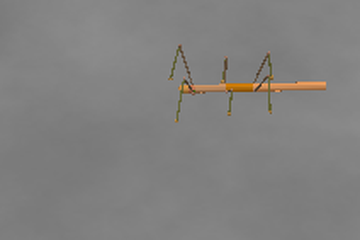
\includegraphics[width=3.1cm]{image/frames/s1_small_0.png} & 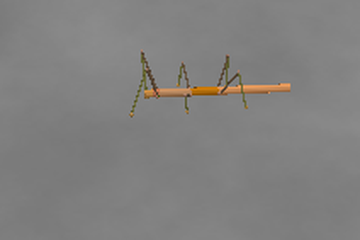
\includegraphics[width=3.1cm]{image/frames/s1_small_30.png} & 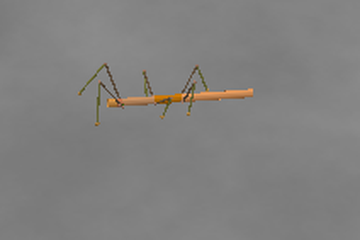
\includegraphics[width=3.1cm]{image/frames/s1_small_60.png} \\
0.6 / 1.0 / 1.0 & 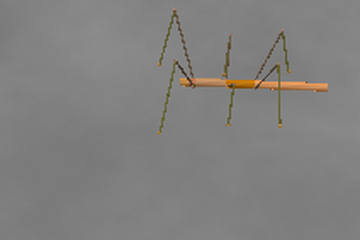
\includegraphics[width=3.1cm]{image/frames/s1_shortcoxa_0.png} & 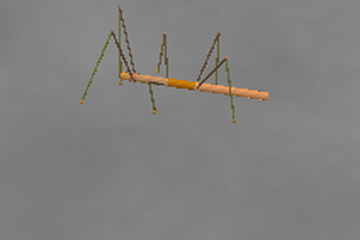
\includegraphics[width=3.1cm]{image/frames/s1_shortcoxa_30.png} & 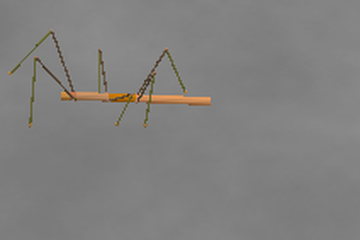
\includegraphics[width=3.1cm]{image/frames/s1_shortcoxa_60.png} \\
(Held-out) 0.8 / 0.9 / 0.9 & 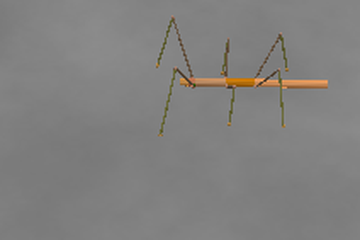
\includegraphics[width=3.1cm]{image/frames/s1_heldout_0.png} & 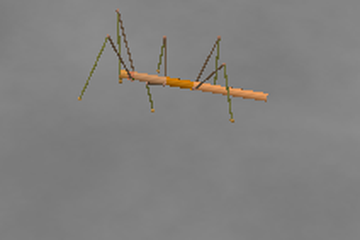
\includegraphics[width=3.1cm]{image/frames/s1_heldout_30.png} & 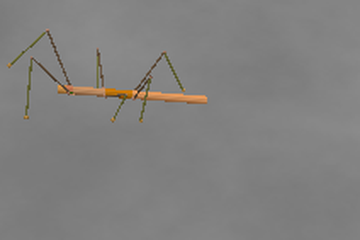
\includegraphics[width=3.1cm]{image/frames/s1_heldout_60.png} \\
1.0 / 1.0 / 1.0 & 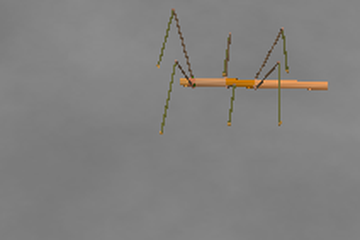
\includegraphics[width=3.1cm]{image/frames/s1_large_0.png} & 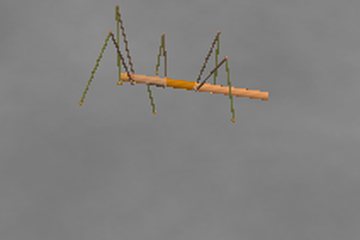
\includegraphics[width=3.1cm]{image/frames/s1_large_30.png} & 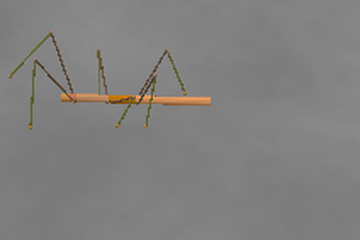
\includegraphics[width=3.1cm]{image/frames/s1_large_60.png} \\
\bottomrule
\end{tabular}
\end{table}

\subsection{Stage 2 Data: Hexapod and B1, Both Cameras}
Stage 2 pairs the hexapod (nominal segment scales, in CoppeliaSim) with the Unitree B1 (a trained walking policy in MuJoCo,
replayed in CoppeliaSim with the same renderer and camera so that both bodies' clips carry the same fields in a common
format). Each body has 12 conditions (4 speeds, 4 turn levels, 4 sideways: left and right at 2 levels), 4 clips per
condition, 48 clips per body; every clip is 66 frames at 20 Hz (3.3 s), 256 $\times$ 256. The 2 bodies name their
conditions differently (for the hexapod a gait parameter, for the B1 a velocity command), so conditions are paired by level, for instance the third turn level of each. The
split per body is 24 train, 12 validation and 12 held-out clips.

Each clip exists under 2 cameras: a fixed third-person view (Table~\ref{tab:data-stage2}) and a head-mounted view in a randomized
textured room (Section 3.2.3, Table~\ref{tab:data-stage2}). Section 3.6.5 uses the same 12 conditions as the
candidate library for closed-loop evaluation.

\begin{table}[H]
\centering
\footnotesize
\renewcommand{\arraystretch}{1.15}
\setlength{\tabcolsep}{2pt}
\caption{Frames from the third turn level of the hexapod and of the Unitree B1, under both cameras.}
\label{tab:data-stage2}
\begin{tabular}{m{2.2cm}>{\centering\arraybackslash}m{2.0cm}>{\centering\arraybackslash}m{2.0cm}>{\centering\arraybackslash}m{2.0cm}@{\hspace{6pt}}>{\centering\arraybackslash}m{2.0cm}>{\centering\arraybackslash}m{2.0cm}>{\centering\arraybackslash}m{2.0cm}}
\toprule
 & \multicolumn{3}{c}{\textbf{Third-person camera}} & \multicolumn{3}{c}{\textbf{Head camera}}\\
\cline{2-4}\cline{5-7}
 & \textbf{0.0 s} & \textbf{1.5 s} & \textbf{3.0 s} & \textbf{0.0 s} & \textbf{1.5 s} & \textbf{3.0 s}\\
\midrule
Hexapod & 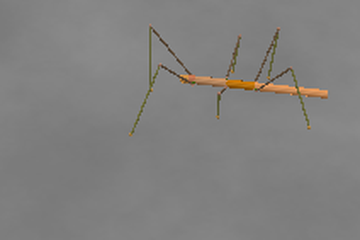
\includegraphics[width=2.0cm]{image/frames/s2_hex_allo_0.png} & 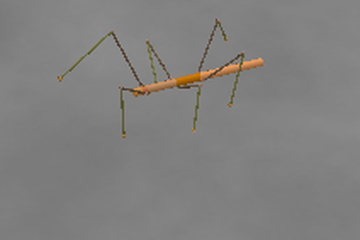
\includegraphics[width=2.0cm]{image/frames/s2_hex_allo_30.png} & 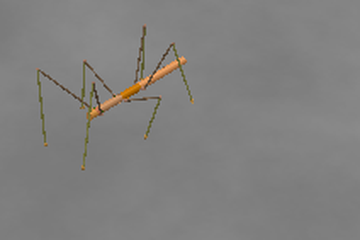
\includegraphics[width=2.0cm]{image/frames/s2_hex_allo_60.png} & 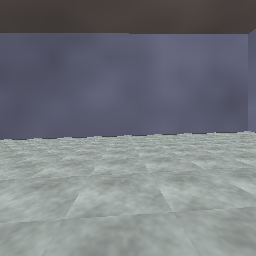
\includegraphics[width=2.0cm]{image/frames/s2_hex_ego_0.png} & 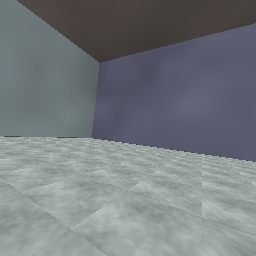
\includegraphics[width=2.0cm]{image/frames/s2_hex_ego_30.png} & 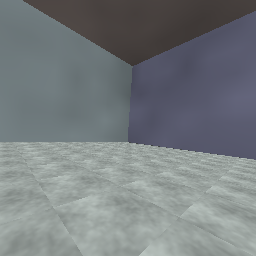
\includegraphics[width=2.0cm]{image/frames/s2_hex_ego_60.png} \\
Unitree B1 & 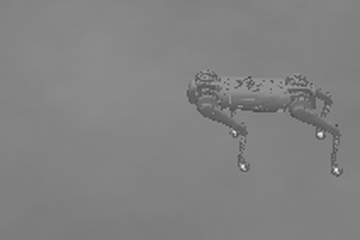
\includegraphics[width=2.0cm]{image/frames/s2_b1_allo_0.png} & 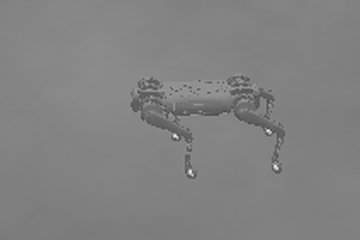
\includegraphics[width=2.0cm]{image/frames/s2_b1_allo_30.png} & 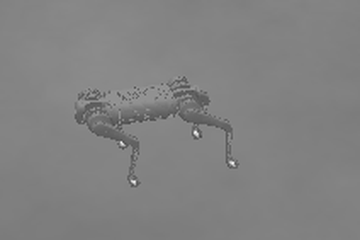
\includegraphics[width=2.0cm]{image/frames/s2_b1_allo_60.png} & 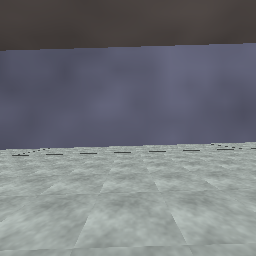
\includegraphics[width=2.0cm]{image/frames/s2_b1_ego_0.png} & 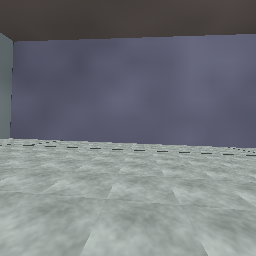
\includegraphics[width=2.0cm]{image/frames/s2_b1_ego_30.png} & 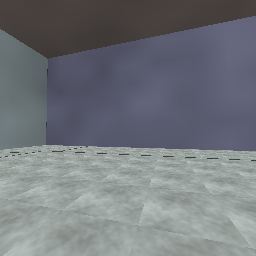
\includegraphics[width=2.0cm]{image/frames/s2_b1_ego_60.png} \\
\bottomrule
\end{tabular}
\end{table}



\subsection{Stage 3 Data: Goal, Candidates and Babble}
\textbf{Goal.} A hexapod clip, one per condition: the 12 held-out clips. It is read at every timestep as a Froude
vector (forward, lateral, yaw), either from the recorded body motion (physics) or from the clip's video (vision).

\textbf{Candidates.} B1 clips only; the goal body is never a candidate. A candidate is scored as
$h_{\text{body}}(\mathrm{Proj}(a))$ against the goal at the same frame index, and the pick is graded against the
candidate's own recorded Froude. 3 libraries are used (Table~\ref{tab:libraries}).

\begin{table}[H]
\centering
\footnotesize
\setlength{\tabcolsep}{4pt}
\caption{The 3 B1 candidate libraries of Stage 3.}
\label{tab:libraries}
\begin{tabularx}{\textwidth}{>{\hsize=0.77\hsize}Y>{\hsize=0.33\hsize\centering\arraybackslash}Y>{\hsize=2.18\hsize}Y>{\hsize=0.72\hsize}Y}
\toprule
\textbf{Library} & \textbf{Clips} & \textbf{How it was made} & \textbf{Recorded at}\\
\midrule
expert (ground-truth) & 24 & trained walking policy in MuJoCo, 12 conditions $\times$ 2 clips & 20 Hz, 66 frames\\
\addlinespace[3pt]
babble \#1 & 36 & MuJoCo CPG with action noise 0.03: 12 forward (1.0, 1.5, 2.0 Hz $\times$ 4 seeds), 12 sideways
  (0.8, 1.0, 1.2 Hz $\times$ 4), 12 turning (pivot 1.2, 1.5, 1.8 $\times$ 4); replayed in CoppeliaSim, one room & 50 Hz, 100 frames\\
\addlinespace[3pt]
babble \#2 & 40 & CoppeliaSim, spring-mode joint control, diagonal trot at 5.0 Hz, amplitude drawn uniformly from
  0.20 to 0.32, action noise 0.03, one seed and one room per clip; forward trot only (clip-mean forward Froude 0.124 to 0.216) & 20 Hz, 160 frames\\
\bottomrule
\end{tabularx}
\end{table}

\subsection{Motor Babble}
The babble libraries follow the recipe of the egocentric visual self-model of Hu et al.\ (Figure~\ref{fig:egovsm}, Section 2.4): a
motor-babbling generator drives the robot, and its egocentric camera records what happens, with no policy, no
kinematic model and no ground-truth demonstration of the body. Figure~\ref{fig:egovsm}a is the collection side, and the
same 3 steps apply here.

\newpage

\begin{enumerate}[label=\arabic*.]
\item \textbf{Generate actions.} An open-loop central pattern generator (CPG) plays the role of the babbling
  generator: 1 sinusoid per leg, with diagonal leg pairs in antiphase, whose frequency, amplitude and seed are drawn
  at random for each clip, with action noise of 0.03 added to every command. The parameters select a behavior
  family: a forward swing, a sideways drive of the hips, or a pivoting differential of the hips that turns the body.
\item \textbf{Execute.} The commands are played on the B1 in the simulator. The generator sees no state of the body
  and reacts to nothing, so falls and awkward gaits stay in the data.
\item \textbf{Record.} The egocentric camera saves the image sequence, and the body's motion is logged as a Froude
  vector for grading only. The clip is then 1 candidate of the library.
\end{enumerate}
2 things differ from Hu et al. First, what is learned from the babble. They fit a self-model, an action encoder and a
visual encoder feeding an MLP that predicts the next state, from scratch for each robot. Here the babble only adapts
the pipeline that was already pretrained on the hexapod (adaptation steps 1 to 3 of Section 3.4.5): steps 1 and 2 are
fitted on the babble library alone and step 3 on the babble library plus the hexapod rehearsal clips. Second, how an
action is chosen (Figure~\ref{fig:egovsm}b). They propose candidate actions, predict each next state with the
self-model and pick the action with the maximum reward. Here the candidates are the recorded babble clips themselves,
each is scored in the Froude coordinate against the goal read from the hexapod's video, and the best-scoring clip is
the pick. The generator here is also more structured than pure random babbling, since randomness enters through the
parameters of a CPG and not through independent random joint commands. The v2 clips are recorded at 50 Hz and the goals at
20 Hz; goal and candidate are matched by frame index, as in the expert library.

\newpage
\section{Evaluation Protocol}

\subsection{Metrics}
2 complementary measures are reported for every latent-structure claim, since reporting only one can mislead:
one for whether information is \emph{present}, one for whether it \emph{dominates} the representation.
Cross-embodiment transfer and the mismatch control that must fail alongside it are measured the same way in both
stages.

\begin{table}[H]
\centering
\footnotesize
\setlength{\tabcolsep}{4pt}
\caption{Metrics used throughout Chapters 3 and 4.}
\label{tab:metrics}
\begin{tabularx}{\textwidth}{>{\hsize=0.85\hsize}Y>{\hsize=1.15\hsize}Y>{\hsize=1.00\hsize}Y}
\toprule
\textbf{Metric} & \textbf{Question it answers} & \textbf{What it measures}\\
\midrule
Linear-probe accuracy & Can a simple classifier decode a label (behavior or embodiment) from the
  representation? & \emph{Presence} of information\\
Silhouette score, between-class variance & Is that information the main axis of variation, or a minor one? &
  \emph{Dominance} of information\\
Cross-embodiment transfer & Does a probe fitted on one embodiment work on the other? & Transfer, always paired
  with a mismatch control that must fail where the real comparison succeeds\\
\bottomrule
\end{tabularx}
\end{table}

The evaluation metrics used in the experiments are defined in Table~\ref{tab:eval-metrics}, so that each result is read against its
definition. $g_t$ is the goal Froude vector (forward, lateral, yaw) at step $t$, $\hat g_t$ the goal as read from video,
$v(c,t)$ the Froude vector of the recorded motion of candidate $c$ over the scored window at step $t$, and
$c^{\star}_t$ the candidate picked at step $t$.

\begin{table}[H]
\centering
\footnotesize
\setlength{\tabcolsep}{6pt}
\renewcommand{\arraystretch}{1.5}
\caption{Evaluation metrics.}
\label{tab:eval-metrics}
\begin{tabularx}{\textwidth}{>{\hsize=0.66\hsize}Y>{\hsize=1.80\hsize}Y>{\hsize=0.54\hsize}Y}
\toprule
\textbf{Metric} & \textbf{Definition} & \textbf{Reads as}\\
\midrule
Held-out ratio & $\dfrac{\mathrm{MSE}(\hat y,\, y)}{\mathrm{MSE}(\bar y,\, y)}$ on the held-out clips, with $\bar y$ the mean of the target & below 1: real signal\\
\addlinespace[3pt]
Correlation $\rho$ & Pearson correlation between the readout and the Froude label, per channel, on the held-out clips (the median over the 3 channels is also reported) & agreement with the label\\
\addlinespace[3pt]
Command recoverability & $R^2$ of a ridge probe from the embedding of 1 frame, or of a frame pair, to the command, held out by clip; the gap is the pair value minus the 1-frame value & what a frame already holds\\
\addlinespace[3pt]
Null/real ratio & $\dfrac{\lVert \hat e^{\,\mathrm{null}}_{t+k} - e_{t+k}\rVert}{\lVert \hat e^{\,\mathrm{real}}_{t+k} - e_{t+k}\rVert}$, where $\hat e^{\,\mathrm{real}}_{t+k}$ is the Forward Transition Model prediction from the real transition and $\hat e^{\,\mathrm{null}}_{t+k}$ the prediction from the null action $\mathrm{ITM}(e_t, e_t)$ & 1.0: action unused\\
\addlinespace[3pt]
Separation & $1-\cos\big(\hat e^{\,\mathrm{real}}_{t+k},\, \hat e^{\,\mathrm{null}}_{t+k}\big)$ & distance between rollouts\\
\addlinespace[3pt]
Froude tracking error & $\dfrac{1}{T}\sum_{t}\big\lVert v(c^{\star}_t, t) - g_t\big\rVert_2$, in real Froude units, graded against the goal the system was given or against the true goal & distance of picks from the goal\\
\addlinespace[3pt]
Goal read error & $\dfrac{1}{T}\sum_{t}\big\lVert \hat g_t - g_t\big\rVert_2$ & cost of reading the goal\\
\addlinespace[3pt]
Best the library could do & the tracking error when the candidate closest to $g_t$ is chosen at every step from the ground truth & ceiling of the library\\
\addlinespace[3pt]
Random pick & the tracking error averaged over all candidates & floor\\
\addlinespace[3pt]
Share of the random-to-best gap recovered & $\dfrac{E_{\text{random}} - E_{\text{selected}}}{E_{\text{random}} - E_{\text{best}}}$ & headroom the scorer uses\\
\addlinespace[3pt]
Regret & $\lVert v(c^{\star}_t, t) - g_t\rVert - \min_c \lVert v(c, t) - g_t\rVert$ & size of a miss\\
\addlinespace[3pt]
Selection accuracy & fraction of decisions whose pick has the goal's behavior family, against the pooled chance rate & coarse selection\\
\bottomrule
\end{tabularx}
\end{table}

\noindent\textbf{Statistical treatment.} Where conditions are compared, the unit of analysis is the condition (the
decisions inside 1 condition are not independent) and differences are paired. Intervals are 95\% bootstrap intervals
over conditions (20{,}000 resamples), tests are the sign test and the Wilcoxon signed-rank test, and proportions carry
Wilson intervals. Each configuration is trained once, so intervals cover the sampling of goals and clips, not the
variance between training runs.

\newpage
\subsection{Definitions of Open-Loop and Closed-Loop Evaluation}
Both terms recur throughout the experiments and are given a precise meaning here rather than used loosely. An \textbf{open-loop} evaluation selects or replays a sequence of actions (or latents) without reading
the body's actual state as the sequence unfolds. Offline selection among recorded conditions
is open-loop in this sense: the video being evaluated already exists, and nothing about the test changes what
happens next in it. A \textbf{closed-loop} evaluation reads the body's actual current state at every step, uses
it to choose the next action, executes that action in the simulator, and repeats on the resulting new state:
\[
\footnotesize
e_t \,\text{(state)} \to \text{selector} \to z_t \to \text{Motion Decoder} \to a_t \to \text{body} \to e_{t+1} \to \cdots
\]
The distinction matters because open-loop replay of a fixed latent sequence desynchronizes on a body whose timing
differs from the one the sequence was recorded on: $z_t$ is a \emph{local} transition, so a demo's $z_t$ (say,
mid-swing) can land on the new body's actual $e_t$ (say, still in stance), an $(e_t, z_t)$ combination the Motion
Decoder never saw during training, producing an unstable command; because gait is cyclic, this drift compounds
rather than self-correcting. Reading the body's real state every step, as the closed loop does, prevents this by
construction. Every result in this chapter states which regime it was measured under.

\subsection{Definitions of In-Distribution and Out-of-Distribution}
``In-distribution'' and ``out-of-distribution'' (OOD) are used on 2 separate axes in this thesis, a body axis
and an action axis, and a result is only meaningful once it is clear which one is meant. Neither is defined by
an output metric such as reconstruction error or $R^2$: both are defined from physical specifications given
before training, so that whether a body or an action is OOD is known in advance of running anything, not read
off how well the model happens to do on it.

\noindent\textbf{Body OOD.} A held-out body is in-distribution if its leg-segment scales lie inside the convex
hull of the training bodies' own scales, and out-of-distribution if they lie outside it (Experiment 1.2). This is
a property of the bodies' geometry alone, fixed before any checkpoint is trained or evaluated.

\noindent\textbf{Action OOD.} A candidate action is in-distribution if it lies within the recorded action range
of the body it was drawn from (the per-joint minimum and maximum observed in that body's own library), and
out-of-distribution otherwise (Section 3.6.5). Action space itself cannot be the shared coordinate that decides
this across embodiments, since it is exactly what is not shared (Section 2.3.1); the recorded range is a
per-body proxy, not a claim that action space generalizes across bodies.

A result that reports the model doing well or poorly on held-out data is not, by itself, a statement about
either axis; it is a statement about generalization only once the held-out condition is located on 1 or both of
these axes, which is why each experiment that reports a held-out result states which body and action range it
was tested inside or outside of.

\subsection{Milestone Gates}
Each stage has gates that its experiments must pass before the next stage relies on them (Table~\ref{tab:gates}). The gates are fixed here, before any result is reported.

\begin{table}[H]
\centering
\footnotesize
\setlength{\tabcolsep}{6pt}
\renewcommand{\arraystretch}{1.5}
\caption{Milestone gates.}
\label{tab:gates}
\begin{tabularx}{\textwidth}{>{\hsize=0.6\hsize}Y>{\hsize=1.4\hsize}Y}
\toprule
\textbf{Gate} & \textbf{Pass criterion}\\
\midrule
\multicolumn{2}{l}{\textbf{Stage 1}}\\
\addlinespace[3pt]
Decoder reads the frame & Given 1 body's frame and another body's latent, the decoder follows the frame's geometry and does not recall the nearest training body\\
\addlinespace[3pt]
Transfer inside the span & Commands predicted for a held-out body inside the training geometry's span walk open-loop, and the boundary of that span is predictable before training\\
\addlinespace[3pt]
\multicolumn{2}{l}{\textbf{Stage 2}}\\
\addlinespace[3pt]
Shared-coordinate transfer & The readout fitted on 1 embodiment transfers to the other in both directions with positive $R^2$, and a goal observed on 1 embodiment's video selects the matching behavior on the other, against chance and a mismatched-goal control\\
\addlinespace[3pt]
Action-conditioning & The forward model's prediction depends measurably more on the true action than on a null action; the camera and the training objective are tested against this gate\\
\addlinespace[3pt]
Ranking & The model orders 2 similar candidate actions by their real outcome, not only grossly different behaviors\\
\bottomrule
\end{tabularx}
\end{table}

\subsection{Primary Evidence and the Value-over-Raw-Command Check}
The \textbf{primary evidence} for the thesis is the shared cross-body head's transfer: does a goal observed on
one embodiment's video, read through $z_t$ and the shared head, select or drive the matching behavior on the
other. This test is clean because it examines the shared coordinate on its own, needs only the held-out
embodiment's video, and does not depend on a comparison against the native command.

\noindent Does the coordinate add value over what a policy can do without it? This is the discipline
applied before crediting the world model with anything: a plain behavior-cloned policy, trained on the
same recorded clips with no world model at all, is the baseline, and any claim that the world model contributes must
beat it, not an arbitrary or a hoped-for one. The raw joint command is a
further, stricter comparison where applicable: obtaining it for a new body requires that body's kinematics, which
the motivating scenario assumes is unavailable, so a latent that matches what the privileged command achieves is
already a substantive result.

\newpage
\subsection{Candidate Generation and the Separation-and-Manifold Constraint}
Every closed-loop evaluation that requires ranking or selecting among actions draws its candidates
from the curated 12-condition library of Section 3.5.2, not from an unconstrained action space, and this is a
methodological constraint stated here so its consequences are reported directly and not left to appear
in the results. 2 properties of a candidate set determine whether ranking is even testable, and
neither is guaranteed by simply having candidates:

\begin{itemize}[label=--]
\item \textbf{Separation.} 2 candidates must produce different, reproducible outcomes for a ranking
  test to mean anything; if the simulator's own execution noise exceeds the gap between 2 candidates' outcomes,
  no ranker, however good, can be shown to distinguish them.
\item \textbf{On-manifold.} What must stay in-distribution is the \emph{behavior} a candidate produces, in the
  Froude-scaled body-motion coordinate of Section 2.3 -- action space cannot be the shared invariant because it is the thing that is not shared
  across embodiments (Section 2.3.1). Because every candidate here is drawn from one body's own recorded action
  library, staying within that body's recorded action range is the practical proxy used to enforce this; a
  perturbation large enough to be trivially separable can leave the trained behavioral distribution well before it
  leaves the action range, at which point a failure to rank it correctly is a failure of generalization to
  unseen behavior, not evidence about ranking within the model's competence.
\end{itemize}

These 2 properties trade against each other: a larger perturbation is easier to separate and more likely to
leave the trained behavioral distribution. 

\chapter{EXPERIMENTS AND RESULTS}

This chapter follows the 3 stages of the research procedure (Section 1.6). Each experiment states its assumption, its input and output, and which objective it answers, then its evidence, the finding, and the gap that remains, so that a result is always read against what it was built to test. Experiment numbers run in the order in which the questions arise: Stage 1 (Experiments 1.1 to 1.3), Stage 2 (Experiments 2.1a, 2.2, 2.4 and 2.3; the 2 independent fixes of the action-use failure are numbered 2.4 for the camera and 2.3 for the objective) and Stage 3 (Experiments 3.1, 3.3, 3.4 and 3.5). The datasets of all 3 stages are declared in Section 3.5.

\noindent\textbf{How to read the numbers.} The held-out sets are small (12 clips per body, and 1 held-out goal clip for each of 12 conditions), and each configuration was trained once, so differences between checkpoints carry no seed variance. Where conditions are compared, the condition is the unit of analysis, since the 30 or so decisions inside 1 condition are not independent; intervals are 95\% bootstrap intervals over conditions, and proportions carry Wilson intervals. Where an interval is not given, the number is a single measurement. Splitting by clip rather than by frame, and holding a body out entirely where the claim is cross-embodiment transfer, is the robustness discipline applied throughout this chapter: a result is not reported until it is checked on data the fitted component never saw. The metrics are defined in Section 3.6.1.

\section{Stage 1: Cross-Morphology on a Shared Joint Space}
Stage 1 is the controlled first step: 9 hexapod bodies that share 1 18-dimensional joint space (Section 3.5.1). It is not a smaller version of Stage 2. It establishes what Stage 2 has to satisfy again without a shared command space to lean on, and it cannot show that vision succeeds where proprioception could not, because a proprioceptive model could in principle be shared across these bodies too. 3 experiments follow. Experiment 1.1 asks whether the decoder reads the frame or recalls the nearest training body, Experiment 1.2 asks where the transfer holds, and Experiment 1.3 asks how much of the command the transition carries beyond the pose.

\subsection{Experiment 1.1: Frame Reading versus Nearest-Body Recall in the Decoder}


\textbf{Assumption:} If the latent truly separates movement from body, a held-out body's commands should come from its own geometry, not a memorized nearby body.


\textbf{Input:} Body A's frame + body B's latent (a forced conflict).

\textbf{Output:} Predicted joint command against body B's true command.


\textbf{Answers:} \textbf{Objective 1}: a verification step, establishing the fix the shared coordinate needs before it can be trusted at all.


\textbf{Dataset:} 9 6-legged walkers (scaling coxa/femur/tibia independently), 30 clips each (270 clips total); 2 bodies dropped for stumbling. \textbf{5 bodies train} (last 1 of 30 clips per body held out internally as validation); the body with segment scales (0.8, 0.9, 0.9) (1 body, all 30 clips) is held out entirely as the unseen-body test; it lies inside the training bodies' convex hull (Experiment 1.2 also runs a second held-out body, with scales (0.6, 0.6, 0.6), that lies outside it).

\begin{quote}
\textbf{Commands are retargeted.} Data used in training takes one foot trajectory in Cartesian space, solved separately for each body by inverse kinematics: same intended behavior, different joint numbers.
\end{quote}

\textbf{Behavior:} forward walking, one speed.


\textbf{The hypothesis.} If the latent truly separates movement from body, then a body never seen in training should receive commands appropriate to its own geometry, not the commands of whichever training body it most resembles.


\begin{center}
\footnotesize
\setlength{\tabcolsep}{3pt}
\begin{tabularx}{\textwidth}{>{\hsize=1.99\hsize}Y>{\hsize=0.59\hsize\centering\arraybackslash}Y>{\hsize=0.71\hsize\centering\arraybackslash}Y>{\hsize=0.71\hsize\centering\arraybackslash}Y}
\toprule
\textbf{held-out body (0.8, 0.9, 0.9)} & \textbf{coxa} & \textbf{femur} & \textbf{tibia} \\
\midrule
the truth & 0.80 & 0.90 & 0.90 \\
\addlinespace[3pt]
probe on the visual encoder (4,227 params) & 0.84 & 0.91 & 0.91 \\
\addlinespace[3pt]
the motion decoder (5.2M params) & 0.62 & 0.96 & 0.96 \\
\bottomrule
\end{tabularx}
\end{center}

The probe lands close everywhere; the decoder implies a coxa 22\% shorter than the body has. The bigger model is the one that misreads it.


Follow-up experiment: is the decoder reading the frame, or recalling the latent's nearest body?


Give the motion decoder body A's frame together with body B's latent. Body B's command differs from body A's by 21$^\circ$. The decoder answers with body B's command to within 6$^\circ$: it follows the latent and ignores the frame.


Expected result : the image should carry which body, the latent should carry what movement. and it would fail outright, because the model never learned the frame-action relationship that idea depends on.


\textbf{The fix is therefore in the objective:} every body shares the same intent and differs only in geometry, so add one loss term that makes that explicit; take body A's latent, show the decoder body B's frame, and require body B's command, that is, minimize
\begin{equation}
\mathcal{L}_{\text{cross}} = \big\lVert \mathrm{MD}\big(e^{B}_t,\, z^{A}_t\big) - a^{B}_t \big\rVert^2,
\end{equation}
where $\mathrm{MD}$ is the Motion Decoder, $z^{A}_t$ body A's latent, $e^{B}_t$ body B's frame embedding and $a^{B}_t$ body B's command.


\begin{center}
\footnotesize
\setlength{\tabcolsep}{3pt}
\begin{tabularx}{\textwidth}{>{\hsize=1.62\hsize}Y>{\hsize=0.79\hsize\centering\arraybackslash}Y>{\hsize=0.59\hsize\centering\arraybackslash}Y}
\toprule
\textbf{held-out body test} & \textbf{without the term} & \textbf{with it} \\
\midrule
command error & 3.67$^\circ$ & 3.44$^\circ$ \\
\addlinespace[3pt]
image's worth to the decoder & 0.4$\times$ & 9.6$\times$ \\
\addlinespace[3pt]
movement's share of the latent & 82\% & 93\% \\
\addlinespace[3pt]
body identity's share of the latent & 12\% & 3\% \\
\bottomrule
\end{tabularx}
\end{center}

\textbf{Finding:} The decoder was recalling the nearest training body, not reading geometry; the cross-body loss term fixes it, validated in-distribution.


\textbf{Remaining gap:} whether the fix holds outside the geometry the training data spans; bridges directly to Experiment 1.2.

\subsection{Experiment 1.2: Transfer Inside versus Outside the Training Geometry's Span}


\textbf{Assumption:} Transfer only holds within the geometric span the training data covers; extrapolation is not assumed to work.


\textbf{Input:} A held-out body's frame.

\textbf{Output:} Predicted joint command (R$^2$ against ground truth), measured inside versus outside the training span.


\textbf{Answers:} Scopes \textbf{Objective 1}  states the condition under which the coordinate is learnable at all.



\begin{center}
\footnotesize
\setlength{\tabcolsep}{3pt}
\begin{tabularx}{\textwidth}{>{\hsize=1.42\hsize}Y>{\hsize=0.80\hsize\centering\arraybackslash}Y>{\hsize=0.70\hsize\centering\arraybackslash}Y>{\hsize=1.19\hsize\centering\arraybackslash}Y}
\toprule
 & \textbf{ground truth (IK)} & \textbf{control} & \textbf{with the cross-body loss} \\
\midrule
forward distance & 100\% & 85\% & 90\% \\
\addlinespace[3pt]
heading deviation & 0$^\circ$ & 11.8$^\circ$ & 5.5$^\circ$ \\
\addlinespace[3pt]
worst joint-limit excursion & 0$^\circ$ & 8.2$^\circ$ & 3.9$^\circ$ \\
\bottomrule
\end{tabularx}
\end{center}

Inside the geometry the training set spans, the predicted commands walk, driven open-loop through the same physics used to collect the data, on a body never trained on.


\begin{center}
\footnotesize
\setlength{\tabcolsep}{3pt}
\begin{tabularx}{\textwidth}{>{\hsize=1.96\hsize}Y>{\hsize=0.52\hsize\centering\arraybackslash}Y>{\hsize=0.52\hsize\centering\arraybackslash}Y}
\toprule
\textbf{same model} & \textbf{error} & \textbf{R$^2$} \\
\midrule
a body with geometry inside the training span & 3.4$^\circ$ & 0.81 \\
\addlinespace[3pt]
a body with femur/tibia ratio outside the training span & 13.4$^\circ$ & $-$0.34 \\
\bottomrule
\end{tabularx}
\end{center}

Outside that span, the same weights fail; proved, not assumed.


\textbf{Test:} same budget, same held-out body, but the training set now contains bodies whose segments do not move together the way every other training body's do.


\begin{center}
\footnotesize
\setlength{\tabcolsep}{3pt}
\begin{tabularx}{\textwidth}{>{\hsize=2.04\hsize}Y>{\hsize=0.65\hsize\centering\arraybackslash}Y>{\hsize=0.65\hsize\centering\arraybackslash}Y>{\hsize=0.65\hsize\centering\arraybackslash}Y}
\toprule
\textbf{same model} & \textbf{coxa} & \textbf{femur} & \textbf{tibia} \\
\midrule
ground truth & 1.00 & 1.00 & 0.80 \\
\addlinespace[3pt]
probe fitted on the original dataset & 0.955 & 0.819 & 0.819 \\
\addlinespace[3pt]
probe fitted on the original dataset + the added bodies & 0.973 & 0.954 & 0.772 \\
\bottomrule
\end{tabularx}
\end{center}

The distance from the held-out body's segment scales to the nearest mixture of the training bodies predicts this failure on its own, no encoder, no model, no learning at all. Every body that cannot be mixed from the training set fails; the one that can, succeeds.


\textbf{A tool this produced:} before committing to a train/held-out split, fit the probe on the training bodies and read off how well it recovers the held-out one. A large error there says the split is asking for a direction the data does not span, and the run will not answer the question meant to be asked; check this before spending the training run, not after.


\textbf{Finding:} Transfer holds inside the training geometry's span, fails outside it, and the failure is predictable in advance from the probe alone.


\textbf{Remaining gap:} whether the action itself matters at all, or the whole prediction is pose-driven; bridges to Experiment 1.3.

\subsection{Experiment 1.3: Command Information in the Transition Beyond the Pose}


\textbf{Assumption:} Gait periodicity may make the pose alone predictive of what comes next, independent of the action; a hypothesis this stage motivates but does not test directly.


\textbf{Input:} The current frame's embedding, with the true transition corrupted or removed.

\textbf{Output:} Predicted command / next embedding.


\textbf{Answers:} motivates \textbf{Objective 3}'s mechanism question.


\begin{center}
\footnotesize
\setlength{\tabcolsep}{3pt}
\begin{tabularx}{\textwidth}{>{\hsize=1.36\hsize}Y>{\hsize=0.64\hsize\centering\arraybackslash}Y}
\toprule
\textbf{what the ITM is given as the next frame} & \textbf{change} \\
\midrule
the true next frame & 3.37$^\circ$ (1$\times$) \\
\addlinespace[3pt]
the current frame again (no transition) & 1.34$\times$ \\
\addlinespace[3pt]
$e_{t-1}$ (wrong transition) & 1.65$\times$ \\
\addlinespace[3pt]
$e_{\text{random}}$ (other time) & 3.44$\times$ \\
\addlinespace[3pt]
$\mathrm{ITM}(\varnothing)$ & 3.48$\times$ \\
\bottomrule
\end{tabularx}
\end{center}

Without the transition, the motion decoder $\mathrm{MD}(e_t, z_t)$ cannot work: $z$ is carrying the movement it needs. A wrong transition hurts \emph{more} than no transition; removing the transition entirely costs 31\% accuracy. The latent action is sensitive to what the second frame contains.



\begin{center}
\footnotesize
\setlength{\tabcolsep}{3pt}
\begin{tabularx}{\textwidth}{>{\hsize=1.04\hsize\centering\arraybackslash}Y>{\hsize=1.04\hsize\centering\arraybackslash}Y>{\hsize=0.87\hsize\centering\arraybackslash}Y>{\hsize=1.04\hsize\centering\arraybackslash}Y}
\toprule
\textbf{steps ahead} & \textbf{$e_{t+h}$} & \textbf{$e_0$} & \textbf{beats $e_0$ by} \\
\midrule
1 & 1.39 & 2.11 & 1.52$\times$ \\
\addlinespace[3pt]
3 & 1.78 & 3.05 & 1.72$\times$ \\
\addlinespace[3pt]
5 & 2.12 & 3.57 & 1.69$\times$ \\
\addlinespace[3pt]
10 & 2.98 & 4.36 & 1.46$\times$ \\
\bottomrule
\end{tabularx}
\end{center}


The claim this section can make, stated narrowly: a gait is a limit cycle, and one frame already shows where in that cycle the body is. 2 pieces of evidence, both direct measurements, neither one a claim about whether the action matters:


(1) One frame already tells which feet are in stance versus swing


\begin{center}
\footnotesize
\setlength{\tabcolsep}{3pt}
\begin{tabularx}{\textwidth}{>{\hsize=0.94\hsize}Y>{\hsize=0.95\hsize}Y>{\hsize=0.95\hsize}Y>{\hsize=1.15\hsize}Y}
\toprule
\textbf{predict from} & \textbf{frame $t$} & \textbf{frames $t$, $t+1$} & \textbf{note} \\
\midrule
$a_{t+1}$ & 5.02$^\circ$ error & 4.54$^\circ$ error & pair helps 1.11$\times$ \\
\addlinespace[3pt]
$a_{t+1}-a_t$ & 2.61$^\circ$ error & 2.40$^\circ$ error & pair helps 1.09$\times$ \\
\addlinespace[3pt]
which feet are swinging & \textbf{0.815} accuracy & 0.840 accuracy & pair barely adds anything \\
\bottomrule
\end{tabularx}
\end{center}

The transition adds almost nothing, 1 frame alone all but settles which feet are down.


(2) The gait is measurably periodic, dominant period $\approx$6.6 frames (offset-sweep spectrum, figure below), a real but secondary $\approx$19.7-frame component.


\begin{figure}[H]
\centering
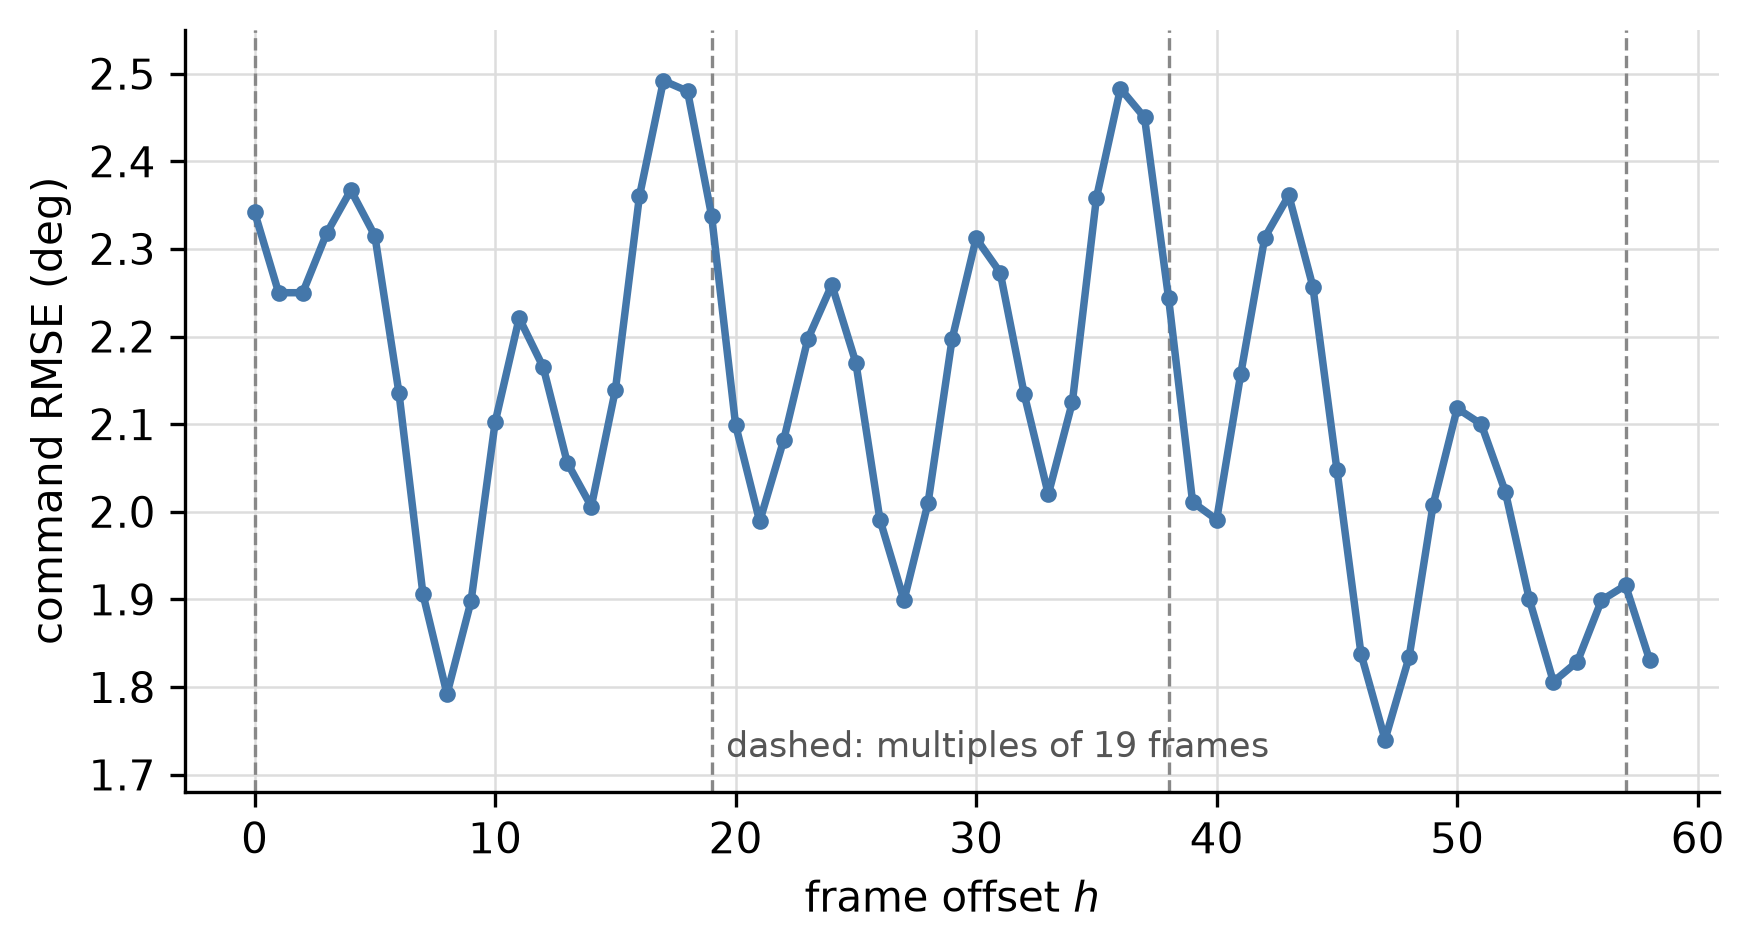
\includegraphics[width=0.7\textwidth]{image/periodicity_curve_fixed_58.png}
\caption{Single-frame command recoverability error (RMSE, degrees) against frame offset, from 0 to 58 frames. Dashed lines mark multiples of the 19-frame gait period.}
\end{figure}


\textbf{(3) The direct test, run on this exact single-embodiment setup, at every horizon from $e_1$ to $e_{16}$:} swap what $z$ the forward model gets, holding the reading otherwise identical. Let $\hat e^{\,\mathrm{real}}_h = \mathrm{FTM}\big(e_0, \mathrm{ITM}(e_0, e_h)\big)$ be the prediction of $e_h$ from the real transition, and $\hat e^{\,\mathrm{null}}_h = \mathrm{FTM}\big(e_0, \mathrm{ITM}(e_0, e_0)\big)$ the prediction from the null action, the latent of a transition in which nothing happened. The table gives the prediction error of each, the error of holding $e_0$ still with no model, and the $\mathrm{null}/\mathrm{real}$ ratio, the null error divided by the real error.


\begin{center}
\footnotesize
\setlength{\tabcolsep}{3pt}
\begin{tabularx}{\textwidth}{>{\hsize=0.85\hsize}Y>{\hsize=1.10\hsize\centering\arraybackslash}Y>{\hsize=1.10\hsize\centering\arraybackslash}Y>{\hsize=0.73\hsize\centering\arraybackslash}Y>{\hsize=1.22\hsize\centering\arraybackslash}Y}
\toprule
\textbf{target} & \textbf{real} & \textbf{null} & \textbf{$e_0$ held still} & \textbf{$\mathrm{null}/\mathrm{real}$} \\
\midrule
$e_1$ & 1.571 & 1.624 & 2.309 & \textbf{1.034} \\
\addlinespace[3pt]
$e_2$ & 1.905 & 2.055 & 2.935 & 1.079 \\
\addlinespace[3pt]
$e_3$ & 2.166 & 2.353 & 3.277 & 1.087 \\
\addlinespace[3pt]
$e_5$ & 2.502 & 2.677 & 3.618 & 1.070 \\
\addlinespace[3pt]
$e_8$ & 2.726 & 2.820 & 3.759 & 1.034 \\
\addlinespace[3pt]
$e_{16}$ & 3.457 & 3.554 & 4.636 & 1.028 \\
\bottomrule
\end{tabularx}
\end{center}

The real action changes prediction error by 3-9\% at every horizon tested, 1 to 16 frames, it reads real structure, it just never needs the action to do it.


\textbf{Finding:} One frame reads gait phase almost as well as a frame pair does (0.815 versus 0.840); the gait is confirmed periodic ($\approx$6.6-frame dominant period); the real action changes prediction error by only 3-9\% at every horizon from 1 to 16 frames.


\textbf{Remaining gap:} why the action helps so little, and whether the same holds when 2 bodies with disjoint action spaces share the model.

\subsection{Stage 1 Summary}
3 requirements come out of Stage 1, each measured on the easy substrate, and each returns as a constraint on the disjoint-action-space pair.

\begin{enumerate}
  \item \textbf{A shared representation has to be forced by the objective, not bought with capacity or architecture.} The motion decoder recalled the nearest training body instead of reading the frame (a coxa 22\% too short on the held-out body). A single cross-body loss term, which makes reading the body out of the latent wrong by construction, raised the image's worth to the decoder from 0.4$\times$ to 9.6$\times$ (Experiment 1.1). Stage 2's shared coordinate is the same move applied where no shared command space exists.
  \item \textbf{Morphology decomposes into several independent axes, and coverage must be verified per axis.} The distance from a held-out body's segment scales to the nearest mixture of the training bodies predicts the failure outside the span on its own, with no encoder, no model and no learning (Experiment 1.2). It is a property of the data, detectable before training at negligible cost. Stage 2 therefore treats embodiment coverage as a per-axis question and not as a body count.
  \item \textbf{A saturating metric conceals what the model is not doing.} At 1 behavior and 1 speed a single frame reads gait phase almost as well as a frame pair (0.815 against 0.840), and the real action changes prediction error by only 3 to 9\% at every horizon from 1 to 16 frames (Experiment 1.3). Every later claim is stated against the mechanism it depends on and not against a proxy for it.
\end{enumerate}

\section{Stage 2: Cross-Embodiment}
Stage 2 adds the Unitree B1, whose action space shares nothing with the hexapod's (Section 3.5.2). It tests the shared Froude coordinate, adapts the model to the B1 in 3 steps, and then asks whether the forward model uses the action it is given.

\subsection{Experiment 2.1a: Necessity of the Shared-Coordinate Loss}


\textbf{Assumption:} a body-motion loss term is necessary to force $z$ to mean the same thing on both bodies; nothing shares that structure for free.


\textbf{Input:} The latent action.

\textbf{Output:} The Cross-Body Head's Froude prediction, R$^2$ measured in all 4 directions (insect/B1 $\times$ insect/B1).


\textbf{Answers:} \textbf{Objective 1} (the coordinate exists) and part of \textbf{Objective 2} (the objective it needs).


Same as Stage 1: a hypothesis, an objective needs to be handed. Froude is the shared target. To force it to be shared across the 2 bodies' latents, add one loss term, read by a single small network shared across both bodies and called the Cross-Body Head


\begin{equation}
\hat{v}_t = h_{\text{body}}(z_t), \qquad \mathcal{L}_{\text{body}} = \lVert \hat{v}_t - v_t \rVert^2,
\end{equation}

where $h_{\text{body}}$ is the Cross-Body Head and $v_t$ the Froude label.

\textbf{Setup.} 1 world model, pretrained jointly on both bodies in a single run. Behavior: forward walking, matched Froude speed across both robots. Both robots are walked at that matched speed, so a readout fitted on one body should work on the other.


\begin{center}
\footnotesize
\setlength{\tabcolsep}{3pt}
\begin{tabularx}{\textwidth}{>{\hsize=1.72\hsize}Y>{\hsize=0.85\hsize\centering\arraybackslash}Y>{\hsize=0.73\hsize\centering\arraybackslash}Y>{\hsize=0.85\hsize\centering\arraybackslash}Y>{\hsize=0.85\hsize\centering\arraybackslash}Y}
\toprule
 & \textbf{insect$\to$insect} & \textbf{b1$\to$b1} & \textbf{insect$\to$b1} & \textbf{b1$\to$insect} \\
\midrule
frozen encoder & 0.676 & 0.753 & $-$0.046 & 0.131 \\
\addlinespace[3pt]
control, no term & 0.664 & 0.167 & $-$7.083 & $-$2.357 \\
\addlinespace[3pt]
+ Cross-Body Head, $\lambda$=0.5 & 0.815 & 0.881 & 0.749 & 0.704 \\
\addlinespace[3pt]
+ Cross-Body Head, $\lambda$=0.1 & 0.809 & 0.868 & 0.675 & 0.624 \\
\bottomrule
\end{tabularx}
\end{center}

Without the term, cross-robot readout is systematically wrong. With it, both directions go positive, and the model is creating structure the encoder did not have.


1 term, 2 wins at once: 38\% better at decoding the robot's own joints, and the same cross-robot.


\begin{center}
\footnotesize
\setlength{\tabcolsep}{3pt}
\begin{tabularx}{\textwidth}{>{\hsize=1.15\hsize}Y>{\hsize=0.74\hsize\centering\arraybackslash}Y>{\hsize=1.11\hsize\centering\arraybackslash}Y}
\toprule
 & \textbf{decode own joints (error)} & \textbf{cross-robot transfer (R$^2$)} \\
\midrule
no body term & 0.3517 & $-$28.9 / $-$43.1 \\
\addlinespace[3pt]
\textbf{+ shared body term} & \textbf{0.2183} & \textbf{+0.610 / +0.573} \\
\bottomrule
\end{tabularx}
\end{center}


``Shared'' versus ``transferred.'' Freeze this same $z$, attach a fresh head, train it on Froude alone: real-$z$ versus mean-$z$ gap +1.048 to +1.226 (bar: 0.110), for both the inverse-model latent and the action-projector latent. A pure normalization artifact would not produce that.


\textbf{Finding:} Without the Cross-Body Head term, cross-robot readout is systematically negative; with it, both directions go positive, and $z$ carries real, usable directional content, not a normalization artifact.

\subsection{Experiment 2.2: Zero-Shot versus 3-Step Adaptation to a Different Robot}


\textbf{Assumption:} pretrained dynamics knowledge transfers to a structurally different body through 3-step adaptation, cheaper than retraining from nothing.


\textbf{Input:} B1's own clips.

\textbf{Output:} Adapted $z$'s correlation ($\rho$) to Froude, per channel, zero-shot versus 3-step.


\textbf{Answers:} \textbf{Objective 2}: correspondence-free transfer, under a specific adaptation procedure.


\textbf{The setup.} Backbone: the hexapod, pretrained across several behaviors and speeds. Question: can that pretrain transfer its behavior understanding to a different robot (B1) by adapting on B1's own clips, rather than retraining from nothing? Measured on a stratified, zero-overlap 24 train / 12 validation / 12 test split per body (all 3 disjoint): 3-step adaptation uses the 24 train clips, ``held-out ratio'' below is scored on the 12 held-out test clips, never touched by any adaptation stage, independently reproduced on 2 machines.



\begin{center}
\footnotesize
\setlength{\tabcolsep}{3pt}
\begin{tabularx}{\textwidth}{>{\hsize=1.22\hsize}Y>{\hsize=1.10\hsize\centering\arraybackslash}Y>{\hsize=0.98\hsize\centering\arraybackslash}Y>{\hsize=0.98\hsize\centering\arraybackslash}Y>{\hsize=0.86\hsize\centering\arraybackslash}Y>{\hsize=0.86\hsize\centering\arraybackslash}Y}
\toprule
\textbf{B1} & \textbf{held-out ratio} & \textbf{forward $\rho$} & \textbf{lateral $\rho$} & \textbf{yaw $\rho$} & \textbf{median $\rho$} \\
\midrule
zero-shot & 1.061 & +0.178 & +0.125 & +0.187 & +0.178 \\
\addlinespace[3pt]
\textbf{Fine tuned} & \textbf{0.730} & \textbf{+0.261} & \textbf{+0.578} & \textbf{+0.474} & \textbf{+0.474} \\
\bottomrule
\end{tabularx}
\end{center}

\begin{center}
\footnotesize
\setlength{\tabcolsep}{3pt}
\begin{tabularx}{\textwidth}{>{\hsize=1.41\hsize}Y>{\hsize=1.06\hsize\centering\arraybackslash}Y>{\hsize=0.94\hsize\centering\arraybackslash}Y>{\hsize=0.94\hsize\centering\arraybackslash}Y>{\hsize=0.82\hsize\centering\arraybackslash}Y>{\hsize=0.82\hsize\centering\arraybackslash}Y}
\toprule
\textbf{hexapod (rehearsal)} & \textbf{held-out ratio} & \textbf{forward $\rho$} & \textbf{lateral $\rho$} & \textbf{yaw $\rho$} & \textbf{median $\rho$} \\
\midrule
Fine tuned & 0.659 & +0.714 & +0.403 & +0.558 & +0.558 \\
\bottomrule
\end{tabularx}
\end{center}

Ratio is MSE against predicting the target's mean: above 1.0 means worse than guessing the average, below 1.0 means real signal.


Zero-shot fails and Fine tuning clearly works and hexapod holds a strong readout throughout rehearsal.


\textbf{The 3-step procedure this uses, assembled from pieces that already existed separately but had never been run as one pipeline before:}


\begin{enumerate}
\item \textbf{Step 1.} Fine-tune only the Inverse and Forward Transition Models on the new body's own clips.
\item \textbf{Step 2.} Fit a separate network, the Action Projector, from action to $z$, which needs no frame pair.
\item \textbf{Step 3.} Refit the Cross-Body Head, with the hexapod clips as rehearsal.
\end{enumerate}
An optional joint fine-tune of all modules exists and is skipped throughout this thesis.

In training, $z = \mathrm{ITM}(e_t, e_{t+1})$, the inverse model reading a real, already-happened frame pair. At the moment a controller executes, the next frame does not exist yet: the projector, $z = \mathrm{Proj}(a)$, exists to supply a $z$ from the action alone, before the outcome is known. Experiment 2.1a's own action-lever check used both $z$ sources side by side for that reason. Same 12 held-out B1 clips, same head, the 2 $z$ sources side by side:


\begin{center}
\footnotesize
\setlength{\tabcolsep}{3pt}
\begin{tabularx}{\textwidth}{>{\hsize=1.28\hsize}Y>{\hsize=1.09\hsize\centering\arraybackslash}Y>{\hsize=0.97\hsize\centering\arraybackslash}Y>{\hsize=0.97\hsize\centering\arraybackslash}Y>{\hsize=0.85\hsize\centering\arraybackslash}Y>{\hsize=0.85\hsize\centering\arraybackslash}Y}
\toprule
\textbf{$z$ source} & \textbf{held-out ratio} & \textbf{forward $\rho$} & \textbf{lateral $\rho$} & \textbf{yaw $\rho$} & \textbf{median $\rho$} \\
\midrule
$\mathrm{ITM}(e_t, e_{t+1})$ & 0.730 & +0.261 & +0.578 & +0.474 & +0.474 \\
\addlinespace[3pt]
$\mathrm{Proj}(a)$ & 0.860 & +0.438 & +0.393 & +0.376 & +0.393 \\
\bottomrule
\end{tabularx}
\end{center}

The control-time path still beats the mean (below 1.0) but is weaker overall (head not refit on projector $z$).


\textbf{How many B1 clips step 3 needs, measured:}


\begin{center}
\footnotesize
\setlength{\tabcolsep}{3pt}
\begin{tabularx}{\textwidth}{>{\hsize=0.91\hsize}Y>{\hsize=1.17\hsize\centering\arraybackslash}Y>{\hsize=1.04\hsize\centering\arraybackslash}Y>{\hsize=1.04\hsize\centering\arraybackslash}Y>{\hsize=0.91\hsize\centering\arraybackslash}Y>{\hsize=0.91\hsize\centering\arraybackslash}Y}
\toprule
\textbf{B1 clips used} & \textbf{held-out ratio} & \textbf{forward $\rho$} & \textbf{lateral $\rho$} & \textbf{yaw $\rho$} & \textbf{median $\rho$} \\
\midrule
3 & 1.530 & +0.169 & +0.191 & +0.359 & +0.191 \\
\addlinespace[3pt]
6 & 0.865 & +0.218 & +0.512 & +0.391 & +0.391 \\
\addlinespace[3pt]
12 & \textbf{0.736} & +0.326 & +0.551 & +0.466 & +0.466 \\
\addlinespace[3pt]
24 (full) & 0.694 & +0.428 & +0.537 & +0.466 & +0.466 \\
\bottomrule
\end{tabularx}
\end{center}

A real cliff, not a curve: 3 clips fails outright; 6 already clears the bar; 12 clips (half the pool) gets within a few points of the full 24. Half the data does most of the job.



\textbf{Finding:} 3-step adaptation takes B1 from failing outright (ratio 1.061) to real signal on every channel (ratio 0.730, median $\rho$ +0.474), on a clean, leak-free, independently reproduced split.


\textbf{Remaining gap:} whether the forward model, now well-calibrated to \emph{read} the action, \emph{uses} it when predicting; bridges to Experiment 2.4.




\textbf{Stage 2's own readout works, but that is a different claim from ``the forward model uses the action'', and the second one is measurably false as things stand.} Swap in a null action ($\mathrm{ITM}(e_t, e_t)$, no real transition at all) for the real one at one prediction step: the forward model's error changes by under 3\% on both robots (real/null ratio 1.03), the model already knows what happens next from the pose alone, whether or not the action it is handed is real. The Cross-Body Head and the forward model are different parts of the network, so Experiments 2.1a--2.2's readout fix says nothing about this. 2 independent fixes address it below.

\subsection{Experiment 2.4a: Pose Sufficiency and Action Redundancy}


\begin{quote}
When the agent's own configuration is visible and determines what happens next, the action carries no information the observation lacks, and a model trained to predict the next observation will ignore it.
\end{quote}

It is not simply ``the agent is in frame.'' Manipulation puts the arm in frame and its world models work. The condition is stronger: the visible configuration must determine the \textbf{future}, not merely reveal the current command.


\begin{figure}[H]
\centering
\begin{minipage}[t]{0.26\textwidth}\centering
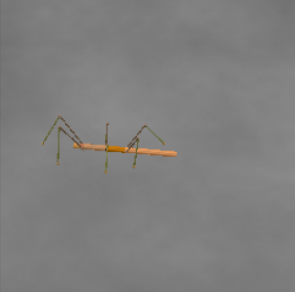
\includegraphics[width=\textwidth]{image/third_person_locomotion.png}
\end{minipage}\hfill
\begin{minipage}[t]{0.30\textwidth}\centering
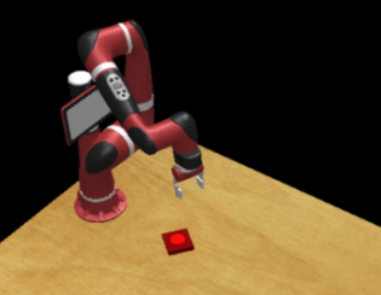
\includegraphics[width=\textwidth]{image/manipulation.png}
\end{minipage}\hfill
\begin{minipage}[t]{0.26\textwidth}\centering
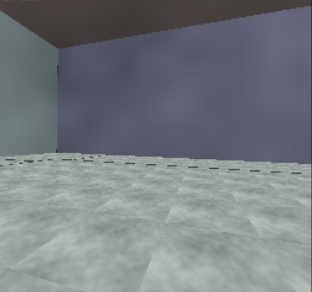
\includegraphics[width=\textwidth]{image/egocentric_locomotion.png}
\end{minipage}
\caption{Third-person locomotion (left), manipulation (middle) and egocentric locomotion (right): whether the visible
configuration determines the future, and so whether the action is redundant.}
\end{figure}

\textbf{Periodicity is what makes locomotion the severe case.} A gait is a limit cycle: the pose fixes the phase and the phase fixes the next pose, so the pose determines not just what the robot is doing but what it is \emph{about to} do, which is the quantity a forward model is trained on.


\textbf{2 interventions separate rhythm from redundancy.} Metric: a ridge probe's command-readability gap, pair R$^2$ minus single-frame R$^2$: does the command become more recoverable from the embedding once a second frame is added? A clean (unbroken) gait is own gap is +0.102 (single-frame R$^2$ 0.729, pair 0.832), the baseline both rows below are read against. This is a readability probe, not the trained forward model itself; it says whether the information is \emph{there} to use, not that anything uses it (that question is the subject of the experiments that follow).


\begin{center}
\footnotesize
\setlength{\tabcolsep}{3pt}
\begin{tabularx}{\textwidth}{>{\hsize=1.96\hsize}Y>{\hsize=1.04\hsize\centering\arraybackslash}Y>{\hsize=0.48\hsize\centering\arraybackslash}Y>{\hsize=0.56\hsize\centering\arraybackslash}Y>{\hsize=0.96\hsize}Y}
\toprule
\textbf{break the gait with} & \textbf{single-frame R$^2$} & \textbf{pair R$^2$} & \textbf{gap} & \textbf{vs. clean gap (+0.102)} \\
\midrule
random command noise (0.02 rad) & 0.383 & 0.581 & \textbf{+0.198} & \textasciitilde{}2x larger \\
\addlinespace[3pt]
real stops/speed changes/turn onsets, gated 2.1--5.6x to confirm they reached the robot & n/a & n/a & \textbf{+0.061} & \emph{smaller}, not larger \\
\bottomrule
\end{tabularx}
\end{center}

So the cause is not rhythm as such: it is whether the command is predictable from the pose at all. Random noise opens the gap because it is exogenous: nothing about the pose predicts noise, so the second frame has to carry it. A real command a controller would issue does not have this property, however non-periodic it is, because the body's own configuration already reflects the intent behind it; confirmed here by the gap going the other way (smaller than the unbroken clean gait, not larger). The next section stops trying to break the gait is rhythm and asks whether hiding the pose entirely (moving the camera) restores the command's readability instead.



\subsection{Experiment 2.4b: Consistency with Published Results}


\emph{does the visible configuration determine the future?}; checked against the literature:


\begin{center}
\footnotesize
\setlength{\tabcolsep}{3pt}
\begin{tabularx}{\textwidth}{>{\hsize=1.5\hsize}Y>{\hsize=0.55\hsize\centering\arraybackslash}Y>{\hsize=0.75\hsize\centering\arraybackslash}Y>{\hsize=0.55\hsize\centering\arraybackslash}Y>{\hsize=1.65\hsize}Y}
\toprule
\textbf{system} & \textbf{agent visible?} & \textbf{pose determines the future?} & \textbf{does it work?} & \textbf{what the principle adds} \\
\midrule
cross-embodiment latent-goal planning (manipulation) & \yes & \no & \yes & why it \emph{can} work: the arm's pose says nothing about where the object ends up, so the action stays informative \\
\addlinespace[3pt]
egocentric locomotion self-model & \no & \no & \yes & why egocentric is necessary, which that paper does not claim \\
\addlinespace[3pt]
static tabletop manipulation & \yes & partly & mixed & names the exception its own authors noted only in passing \\
\addlinespace[3pt]
ours, third-person locomotion & \yes & \yes (the gait is a limit cycle) & \no & this is the collapse, measured end to end \\
\bottomrule
\end{tabularx}
\end{center}

The general version of this problem has a name and a proposed fix in the literature. UWM-JEPA (arXiv 2605.25313) names this failure mode: a teacher-forced prediction target already contains the action's effect, which ``admits an action-invariant solution''; the model can satisfy the training objective while ignoring the action channel entirely, whenever the target it is scored against lets it. Their own fix is counterfactual targets (never run here; a different route than either fix this thesis takes); the diagnosis is the same one this project measured directly for locomotion (Experiment 1.3): if the model is not prevented from reading the answer off context it already has, nothing forces it to use the action at all.


\textbf{The prediction, tested.} If \emph{pose determines the future} is what kills action-conditioning, then removing the agent's own pose from view should restore it; this is the first of 2 independent fixes, the other being an objective-side one (Experiment 2.3). What follows tests it directly.

\subsection{Experiment 2.4c: Egocentric Camera Intervention}


\textbf{Assumption:} if pose visibility is what kills action-conditioning, removing the agent's own pose from view should restore it.


\textbf{Input:} Egocentric video.

\textbf{Output:} Command recoverability (R$^2$) and the shared coordinate's own readout, before versus after the camera move.


\textbf{Answers:} \textbf{Objective 3}: the mechanism, and one of its 2 independent fixes.


\textbf{The cheapest test that could answer it, built to be discarded:} 4 textured walls and a ceiling around the spawn point, camera moved onto the robot's head. Not an environment.


\textbf{A robustness check ran first, and the result was not read until it passed:} room appearance predicts heading \textbf{below chance} on held-out clips, on both bodies. Nothing is being read off the wallpaper.


\begin{center}
\footnotesize
\setlength{\tabcolsep}{3pt}
\begin{tabularx}{\textwidth}{>{\hsize=1.04\hsize}Y>{\hsize=1.06\hsize\centering\arraybackslash}Y>{\hsize=0.90\hsize\centering\arraybackslash}Y}
\toprule
\textbf{command recoverable from, 6-legged insect} & \textbf{third-person} & \textbf{egocentric} \\
\midrule
single frame & \textbf{0.78} & \textbf{0.29} \\
\addlinespace[3pt]
a frame pair & 0.89 & 0.58 \\
\addlinespace[3pt]
\textbf{what the transition adds} & +0.11 & \textbf{+0.29} \\
\bottomrule
\end{tabularx}
\end{center}

Single-frame readability falls by 2 thirds, and the transition's value nearly triples. Sideways motion reads \textbf{nothing at all} from one egocentric frame, against 0.61 third-person.**


Does it break cross-body result Fitted on the insect's egocentric observations and applied to the quadruped with no refitting at all:


\begin{center}
\footnotesize
\setlength{\tabcolsep}{3pt}
\begin{tabularx}{\textwidth}{>{\hsize=1.53\hsize}Y>{\hsize=0.94\hsize\centering\arraybackslash}Y>{\hsize=0.94\hsize\centering\arraybackslash}Y>{\hsize=0.59\hsize\centering\arraybackslash}Y}
\toprule
\textbf{the shared coordinate, quadruped unrefitted} & \textbf{forward} & \textbf{lateral} & \textbf{turn} \\
\midrule
third-person & 0.63 & 0.43 & \textbf{0.07} \\
\addlinespace[3pt]
\textbf{egocentric} & 0.50 & 0.39 & \textbf{0.64} \\
\bottomrule
\end{tabularx}
\end{center}

Turning improved the most: a head camera sees rotation as global image flow whatever body is underneath. Forward and lateral fall. The coordinate is harder to read from a head view and it still crosses; that trade is the honest summary.




\textbf{this proves} : action is less redundant with the pose frame. It does \textbf{not} show that a trained world model then uses the transition.


\textbf{Finding:} Egocentric view cuts single-frame recoverability by 2-thirds, and the cross-body still survives.


\textbf{Remaining gap:} with no action to see from frame, will the FTM predict better.

\subsection{Experiment 2.4d: Effect of the Egocentric Camera}


Egocentric true strength, against chance and against the allocentric baseline:


First row, defined here since this is its first appearance: $\mathrm{null}/\mathrm{real}$ = prediction error with a null (uninformative, $\mathrm{ITM}(e_t, e_t)$) action, divided by error with the real recorded one. 1.0 means the real action changes nothing. On the original (allocentric/third-person) camera this sits at \textbf{1.03} (real action worth under 3\%, both robots): the concrete evidence behind Experiment 2.2's closing claim that the forward model ignores the action as things stand.


\begin{center}
\footnotesize
\setlength{\tabcolsep}{3pt}
\begin{tabularx}{\textwidth}{>{\hsize=1.56\hsize}Y>{\hsize=0.89\hsize}Y>{\hsize=0.81\hsize}Y>{\hsize=0.74\hsize}Y}
\toprule
\textbf{can it...} & \textbf{allocentric} & \textbf{egocentric} & \textbf{verdict} \\
\midrule
does the prediction depend on the action at all ($\mathrm{null}/\mathrm{real}$ ratio) & 1.03 & 1.16 insect $\cdot$ 1.08 B1, one step & \textbf{fixed} \\
\addlinespace[3pt]
read ego-motion in the shared coordinate (turn) & 0.07 & 0.64 & \textbf{fixed} \\
\addlinespace[3pt]
order 2 similar actions within one behavior & 4/12 = 33\% (chance 50\%) & 7/15 = 47\% & \textbf{not shown to be fixed} \\
\addlinespace[3pt]
order 2 different behaviors & 55\% (chance 33\%) & 52\% & \textbf{unchanged} \\
\addlinespace[3pt]
recover the command from (frame, z) & 0.982 & 0.847 & \textbf{$-$14\%} \\
\bottomrule
\end{tabularx}
\end{center}

Whether the forward model's prediction \emph{depends} on the action at all is the core action-blindness problem addressed in this chapter, and it is fixed here.


Ordering 2 similar actions within 1 behavior is a different capability entirely, resolving which of 2 nearly-identical outcomes an action leads to, and egocentric do not fix it. A model can attend to the action channel and still be unable to resolve a small difference in where that action leads.

\subsection{Experiment 2.3: Context Collapse and Action Separation}


\textbf{Assumption:} context collapse is fixable by anchoring prediction over the same horizon the separation hinge acts on, not by reweighting the loss alone.


\textbf{Input:} A frame's embedding plus the real or a null action.

\textbf{Output:} Rolled prediction error, real-vs-null separation.


\textbf{Answers:} \textbf{Objective 3}: the mechanism, an algorithm-level fix on this pretrain, checked on its own terms.


Where this starts: the command is already readable from 1 frame (R$^2$, ridge regression).


\begin{center}
\footnotesize
\setlength{\tabcolsep}{3pt}
\begin{tabularx}{\textwidth}{>{\hsize=1.50\hsize}Y>{\hsize=0.75\hsize\centering\arraybackslash}Y>{\hsize=0.75\hsize\centering\arraybackslash}Y}
\toprule
\textbf{command recoverable from} & \textbf{one frame R$^2$} & \textbf{a frame pair R$^2$} \\
\midrule
6-legged insect & \textbf{0.78} & 0.89 \\
\addlinespace[3pt]
of which turning only & \textbf{0.93} & 0.96 \\
\addlinespace[3pt]
quadruped & 0.16 & 0.34 \\
\bottomrule
\end{tabularx}
\end{center}

\textbf{Citation.} Yeom et al., arXiv 2606.07687: frozen V-JEPA carries recoverable action structure; CALVIN's static scene lets one frame substitute for a pair. Same substitution here: 88\% (0.78/0.89), 97\% turning (0.93/0.96), 47\% quadruped (0.16/0.34).


\textbf{The actual problem.} Real action versus null action through the forward model: prediction error changes by under 3\%. Context collapse (ActSWM, 2607.26712).




\textbf{Diagnosis: the objective does not force separation far enough forward.} The pretraining loss separates a real action's rolled-forward prediction from a null action's over a multi-step window (the hinge), but only anchors prediction accuracy at step 1; nothing stops steps 2 and beyond from diverging just to satisfy that separation cheaply.


\textbf{Fix.} The 3 terms defined in Section 3.1 are added: the hinge ($\lambda_{\text{hinge}}=0.5$, horizon $K=2$, margin $m=0.1$), the frozen readout ($\lambda_{\text{readout}}=1.0$) and the 2-step rollout loss ($\lambda_{\text{rollout}}=1.0$). The rollout loss is the anchor the hinge needs: with the hinge and the readout alone, rollout error was 3 to 4$\times$ worse than a frozen frame by step 2, because the reconstruction loss only anchors step 1 and steps 2 and beyond were unopposed.

\begin{center}
\footnotesize
\setlength{\tabcolsep}{3pt}
\begin{tabularx}{\textwidth}{>{\hsize=0.92\hsize}Y>{\hsize=1.13\hsize}Y>{\hsize=0.95\hsize}Y}
\toprule
\textbf{measurement} & \textbf{before this fix} & \textbf{after this fix} \\
\midrule
rollout error/a frozen frame & 0.74 at step 1, climbing to \textbf{3.1--3.3$\times$} by steps 2--5 & flat at \textbf{0.52--0.58$\times$}, holds through step 10 \\
\addlinespace[3pt]
real-vs-null separation, over training & rises then collapses: 0.02 $\to$ 0.14 $\to$ 0.50 $\to$ \textbf{0.008} & rises \textbf{0.0007 $\to$ 0.35} and holds \\
\bottomrule
\end{tabularx}
\end{center}

Both measured directly on the hexapod pretrain itself; this fix's own, confirmed result.


\textbf{Combined with the camera fix of Experiment 2.4, not separate from it:} the checkpoint used from Experiment 2.2 onward is trained on egocentric data with the hinge, readout and rollout terms together ($\lambda_{\text{hinge}}=0.5$, $\lambda_{\text{readout}}=1.0$, $\lambda_{\text{rollout}}=1.0$). Real-vs-mean gap: B1 \textbf{+0.978}, hexapod \textbf{+0.686} (bar: 0.110).


\textbf{And $\mathrm{null}/\mathrm{real}$ holds on this exact combined checkpoint, not just egocentric alone:}


\begin{center}
\footnotesize
\setlength{\tabcolsep}{3pt}
\begin{tabularx}{\textwidth}{>{\hsize=0.58\hsize\centering\arraybackslash}Y>{\hsize=1.15\hsize\centering\arraybackslash}Y>{\hsize=1.27\hsize}Y}
\toprule
\textbf{lag} & \textbf{$\mathrm{null}/\mathrm{real}$} & \textbf{reading} \\
\midrule
1 & 1.062 & action buys something \\
\addlinespace[3pt]
2 & 1.106 & \textbf{viable} \\
\addlinespace[3pt]
3 & 1.115 & \textbf{viable} \\
\addlinespace[3pt]
5 & 1.109 & \textbf{viable} \\
\addlinespace[3pt]
8 & 1.093 & action buys something \\
\bottomrule
\end{tabularx}
\end{center}

Comfortably clear of the 1.03 allocentric floor at every lag: the fixes combine rather than trade off (unlike a rejected loss term elsewhere in this project that improved other metrics while $\mathrm{null}/\mathrm{real}$ silently fell back to \textasciitilde{}1.0).


\textbf{Finding:} The multi-step anchor fix passes all 3 pre-registered criteria, and $\mathrm{null}/\mathrm{real}$ holds up on the fully combined checkpoint at every lag tested.


\textbf{Remaining gap:} true performance in execute control loop.

\section{Stage 3: Closed Loop and Controllers}
Stage 3 asks what the resulting model can do in a closed loop. Its goal, candidate libraries and babble libraries are declared in Section 3.5.3.

\subsection{Stage 3 Overview}
Stage 3 asks what the model can do once a goal has to be met. It is a preliminary study: it tests whether scoring in Froude space, and not in frame space, works when the model is given something to choose between. Frame and embedding distance were tried first and got almost nothing (18 to 23\%, barely above the 28\% chance floor), because that space carries much that has nothing to do with the dynamics. The shared Froude coordinate replaces it.

A goal can be met by 2 mechanisms, which differ in what the action is allowed to be (Table~\ref{tab:mechanisms}). Action selection ranks candidates from a recorded library and is what Experiments 3.3 and 3.4 test. An RL policy needs a reward that can tell a locally better action from a slightly worse one, and that ability is checked directly and currently fails: at or below chance on B1 (1.0 to 2.1\% against 3.0\% chance, large-sample re-test). A teacher-graded policy, which clones the expert and then perturbs and scores around its own action, is still action selection underneath and inherits the same ranking limit. Experiment 3.1 tests an imagination-trained policy, the one route here that does not score discrete candidates.

\begin{table}[H]
\centering
\footnotesize
\setlength{\tabcolsep}{4pt}
\caption{The 2 mechanisms for meeting a goal.}
\label{tab:mechanisms}
\begin{tabularx}{\textwidth}{>{\hsize=0.5\hsize}Y>{\hsize=1.4\hsize}Y>{\hsize=1.1\hsize}Y}
\toprule
 & \textbf{Action selection (coarse)} & \textbf{RL policy (fine)}\\
\midrule
What it can do & Pick or rank any candidate against a recorded library, a whole clip or a small variation within one; bounded by the library, it cannot produce an action that is not in it & Choose any continuous action from the full action space; not bounded by a library\\
\addlinespace[3pt]
What it needs & A library of actions of the new body & Nothing recorded for the goal itself; the behavior is reconstructed by exploring against the world model\\
\bottomrule
\end{tabularx}
\end{table}

\subsection{Experiment 3.1: Imagination-RL}


\textbf{Assumption:} an actor-critic trained against the frozen world model's imagined rollouts can learn to value nearby futures well enough to drive a policy, if the imagination horizon and the critic's own grounding are matched to how far the model's own rollout stays reliable.


\textbf{Input:} Imagined rollout.

\textbf{Output:} Critic value $\to$ policy gradient.


\textbf{Answers:} \textbf{Objective 3}: this is the first result of its kind where the actor's return under the model's own Froude reading converges and holds, not just a training-time proxy.


\textbf{Setup: frozen FTM, one fixed real (start, goal) pair, no re-grounding.} The reward is the negative L1 distance between the Froude reading of the action, $h_{\text{body}}(\mathrm{Proj}(a))$, and one fixed goal vector, in standardized units. How far ahead the FTM's own rollout stays reliable was measured directly (auto-regressive, versus a ``predict no change'' baseline):


\begin{figure}[H]
\centering
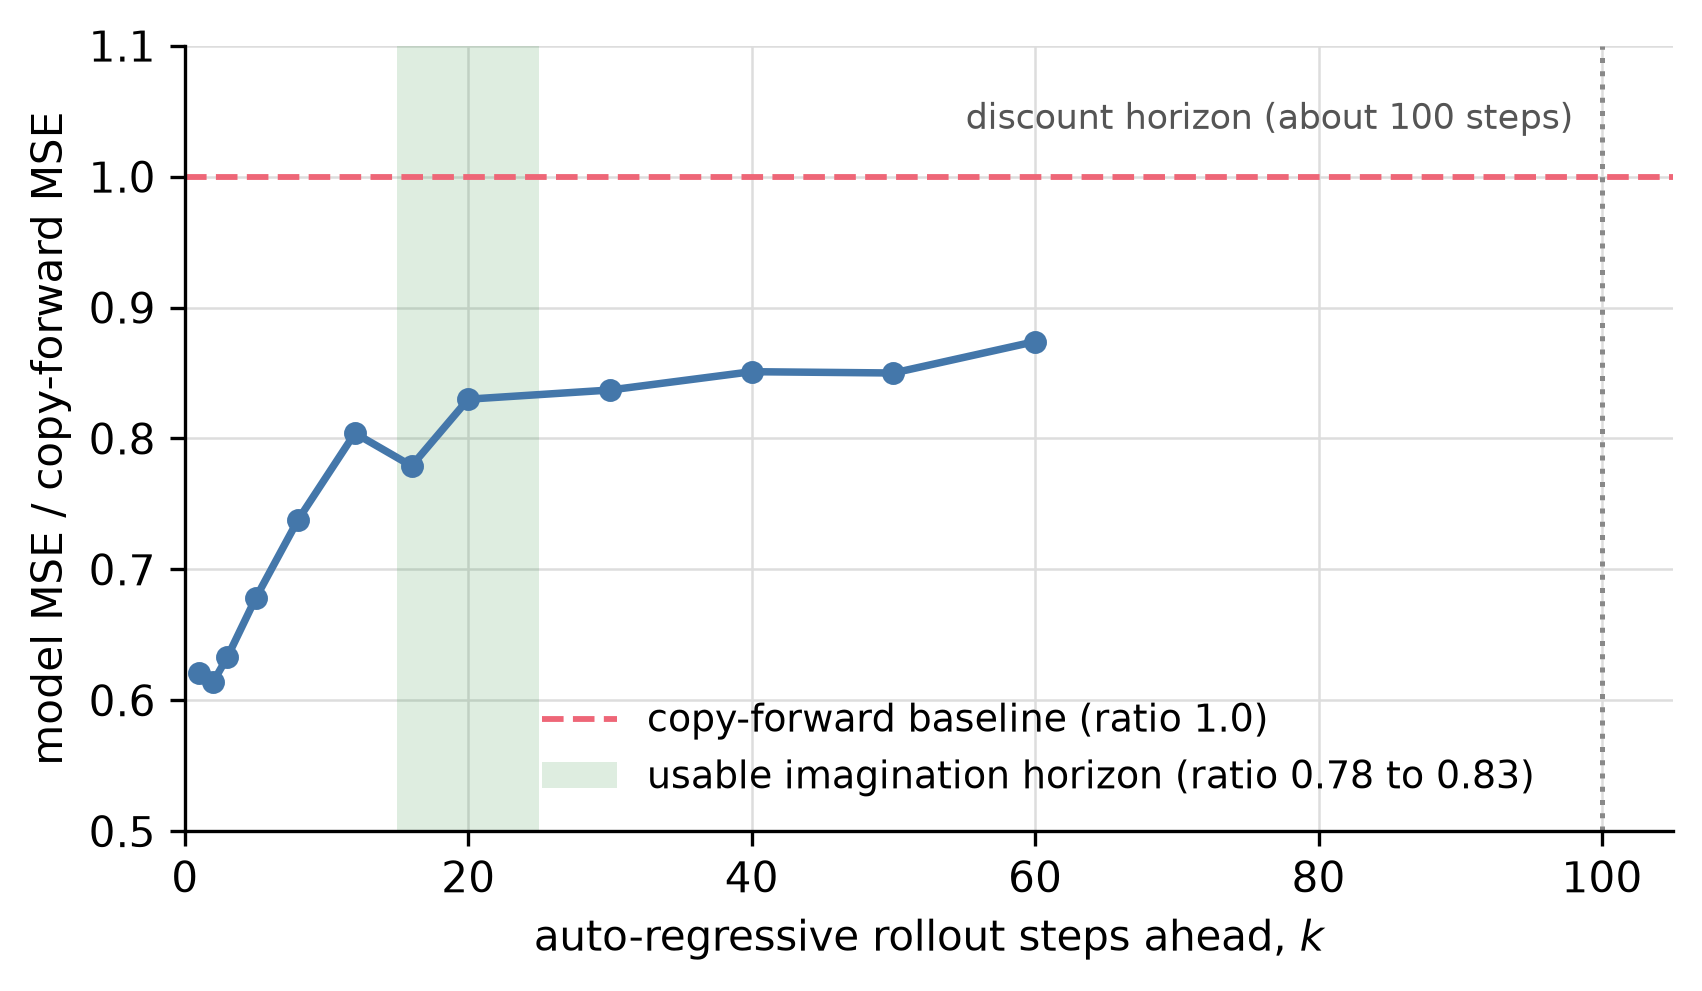
\includegraphics[width=0.7\textwidth]{image/rollout_horizon_accuracy.png}
\caption{Ratio of the Forward Transition Model's rollout error to the copy-forward baseline against rollout length, on B1 data. Values below 1.0 mean the rollout still beats predicting no change.}
\end{figure}


Ratio stays below 1.0 (never worse than doing nothing) out to k=60, but the model's edge is already thin (0.80--0.84) by k=20-30. Horizon picked from this curve: H=12.


\textbf{Recipe: H=12, symlog critic + return normalization, periodic reset to a real Monte Carlo return} (every 200 iterations: roll the current policy forward for real, no critic involved, regress the critic onto that one number, hard-copy the target network from it).


\begin{center}
\footnotesize
\setlength{\tabcolsep}{3pt}
\begin{tabularx}{\textwidth}{>{\hsize=0.58\hsize\centering\arraybackslash}Y>{\hsize=1.04\hsize\centering\arraybackslash}Y>{\hsize=1.38\hsize}Y}
\toprule
\textbf{iter} & \textbf{realized return (actor)} & \textbf{independent MC-return, measured fresh at each anchor} \\
\midrule
0 & $-$15.4 & $-$22.2 \\
\addlinespace[3pt]
200 & $-$6.5 & $-$10.4 \\
\addlinespace[3pt]
600 & $-$2.7 & $-$4.3 \\
\addlinespace[3pt]
1200 & $-$2.7 & $-$4.4 \\
\addlinespace[3pt]
1999 & $-$2.7 & (150 iters past last anchor) \\
\bottomrule
\end{tabularx}
\end{center}

\begin{figure}[H]
\centering
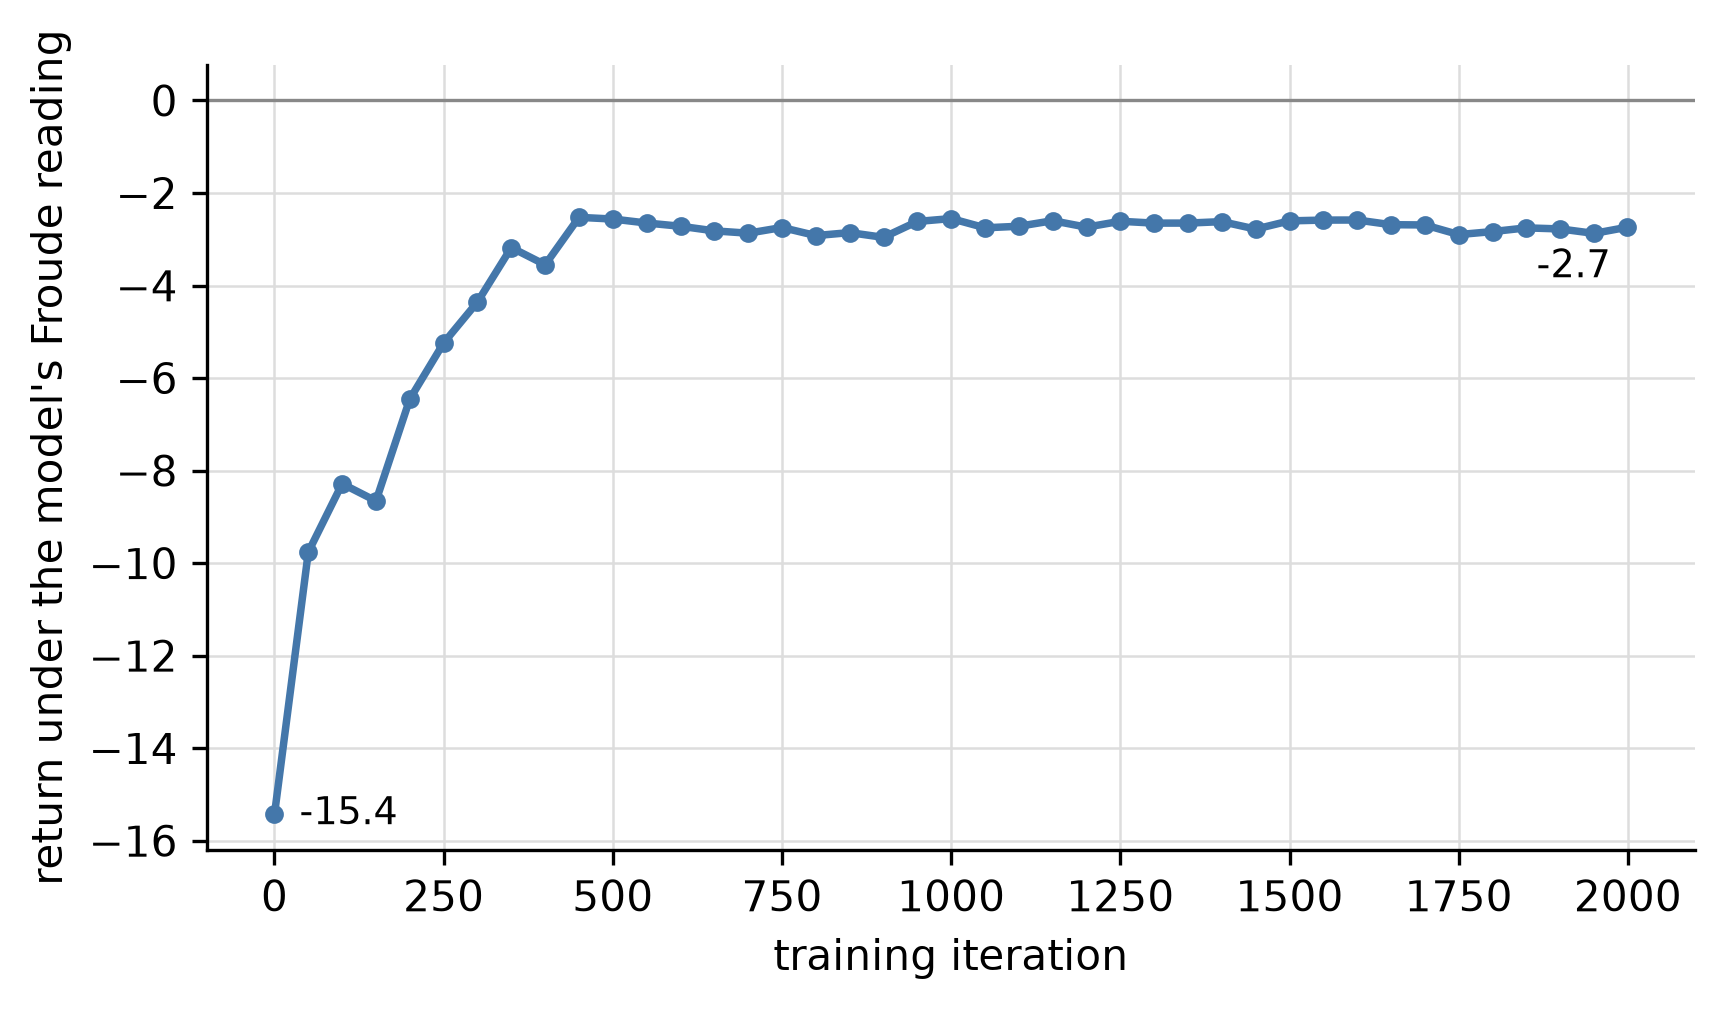
\includegraphics[width=0.7\textwidth]{image/rl_anchor_convergence.png}
\caption{Return of the imagination-RL actor on the fixed start and goal, measured under the model's Froude reading, over 2{,}000 training iterations.}
\end{figure}


2 independent measurements, one fast (12-step training rollout), one slow and bootstrap-free (20-step Monte Carlo), agree the policy improves and then holds, not just on one proxy metric.


\textbf{Scope.} This result is for one fixed start state and one fixed goal: the isolation test's own deliberate design. Extended to 12 diverse (start, goal) tasks with a goal-conditioned actor/critic, same recipe: train-pool and held-out-pool returns stay essentially flat (\textasciitilde{}$-$30 $\to$ \textasciitilde{}$-$29/$-$30) over the same budget: the single-pair result has not yet been shown to generalize.


\textbf{Finding:} The recipe converges to a stable policy on the single-pair isolation test, judged by the return under the model's own Froude reading: the first time in this work. That reading does not depend on the imagined rollout, and it has not yet been shown to generalize past one pair or to hold in physics.


\textbf{Remaining gap:} whether more budget, a larger network, or more tasks per anchor point closes the generalization gap; untested, not ruled out.

\subsection{Experiment 3.3: Scoring in the Shared Coordinate versus Raw Frame Distance}


\textbf{Assumption:} scoring candidates in the shared Froude coordinate, not raw frame/embedding distance, is what a working closed loop needs.


\textbf{Input:} A candidate library plus a goal.

\textbf{Output:} Selection accuracy, frame-distance versus Froude-distance scoring.


\textbf{Answers:} \textbf{Objective 3}: establishes action selection (the coarse mechanism, Stage 3's own intro) as working.


\textbf{Setup : the goal is read fresh every timestep (the goal Froude at that step)} ; horizons 3/5/10 average a candidate's own short execution window against the matching window of the goal, the same way a controller running that many open-loop steps would be judged.


\textbf{Scoring in the right space is what turned selection on.} Frame distance reads the current frame, not the goal. Rescoring by body-motion (Froude) distance fixes that immediately.


\begin{center}
\footnotesize
\setlength{\tabcolsep}{3pt}
\begin{tabularx}{\textwidth}{>{\hsize=1.17\hsize}Y>{\hsize=0.80\hsize}Y>{\hsize=1.02\hsize}Y}
\toprule
\textbf{selection rule} & \textbf{same-robot} & \textbf{cross-embod., 3ch} \\
\midrule
frame/embedding distance & 18-23\% (28\% chance) & n/a \\
\addlinespace[3pt]
\textbf{Froude distance, no rollout} & \textbf{76-86\%} & \textbf{68-70\%} \\
\addlinespace[3pt]
+ FTM rollout added back & n/a & 33-44\%, turning destroyed \\
\bottomrule
\end{tabularx}
\end{center}

\begin{center}
\footnotesize
\setlength{\tabcolsep}{3pt}
\begin{tabularx}{\textwidth}{>{\hsize=0.82\hsize\centering\arraybackslash}Y>{\hsize=1.27\hsize}Y>{\hsize=0.91\hsize\centering\arraybackslash}Y}
\toprule
\textbf{strafing} & \textbf{1-channel} & \textbf{3-channel} \\
\midrule
 & 13-25\% (17\% chance) & \textbf{86-100\%} \\
\bottomrule
\end{tabularx}
\end{center}

\noindent How close is a ``miss,'' in real units


\textbf{regret}: the true distance-to-goal of the candidate picked, minus the true distance-to-goal of the best real candidate available: real (forward/lateral/yaw) Froude units, ground truth on both sides, no model prediction involved in the grading itself.


\begin{center}
\footnotesize
\setlength{\tabcolsep}{3pt}
\begin{tabularx}{\textwidth}{>{\hsize=1.09\hsize\centering\arraybackslash}Y>{\hsize=1.23\hsize\centering\arraybackslash}Y>{\hsize=1.23\hsize\centering\arraybackslash}Y>{\hsize=0.82\hsize\centering\arraybackslash}Y>{\hsize=0.68\hsize\centering\arraybackslash}Y>{\hsize=0.95\hsize\centering\arraybackslash}Y}
\toprule
\textbf{horizon} & \textbf{sideways left} & \textbf{sideways right} & \textbf{speed} & \textbf{turn} & \textbf{\textbf{mean regret}} \\
\midrule
1 & 78\% & 83\% & 20\% & 47\% & \textbf{0.041} \\
\addlinespace[3pt]
3 & 76\% & 80\% & 24\% & 55\% & \textbf{0.032} \\
\addlinespace[3pt]
5 & 73\% & 93\% & 14\% & 64\% & \textbf{0.034} \\
\addlinespace[3pt]
10 & 92\% & 84\% & 11\% & 70\% & \textbf{0.026} \\
\bottomrule
\end{tabularx}
\end{center}

The \emph{speed} family is named wrongly most of the time (11-24\%), but its regret is still small: the candidate it picks stays close to the true best one in real units, even when graded a miss.


Longer horizon scores better because it averages out noise, shorter horizon might be wobble in the gait and the reading shifts. Horizon 10 averages the candidate's own motion over 10 frames, which cancels that noise and leaves the sustained direction. Regret falls 0.041$\to$0.026 and family accuracy rises as horizon grows for this reason.



\noindent Limitation: telling similar actions apart, not tracking a moving goal


Picking the right action works. Telling 2 \emph{nearly identical} actions apart does not.


\begin{center}
\footnotesize
\setlength{\tabcolsep}{3pt}
\begin{tabularx}{\textwidth}{>{\hsize=1.13\hsize}Y>{\hsize=0.87\hsize}Y}
\toprule
\textbf{question} & \textbf{result} \\
\midrule
walk / turn / strafe & works, crosses embodiments \\
\addlinespace[3pt]
0.5-sd perturbations of one behavior, pick the closer & 7/15 = 47\% vs a 50\% coin \\
\bottomrule
\end{tabularx}
\end{center}



\textbf{Finding:} Froude-space scoring turns selection on; wrong picks stay close in real units (regret). Telling nearly-identical actions apart stays near chance regardless of representation tried.


\textbf{Remaining gap:} isolating which half of the closed loop, goal or scoring, is broken.

\subsection{Controller and Test Regime}


\begin{figure}[H]
\centering
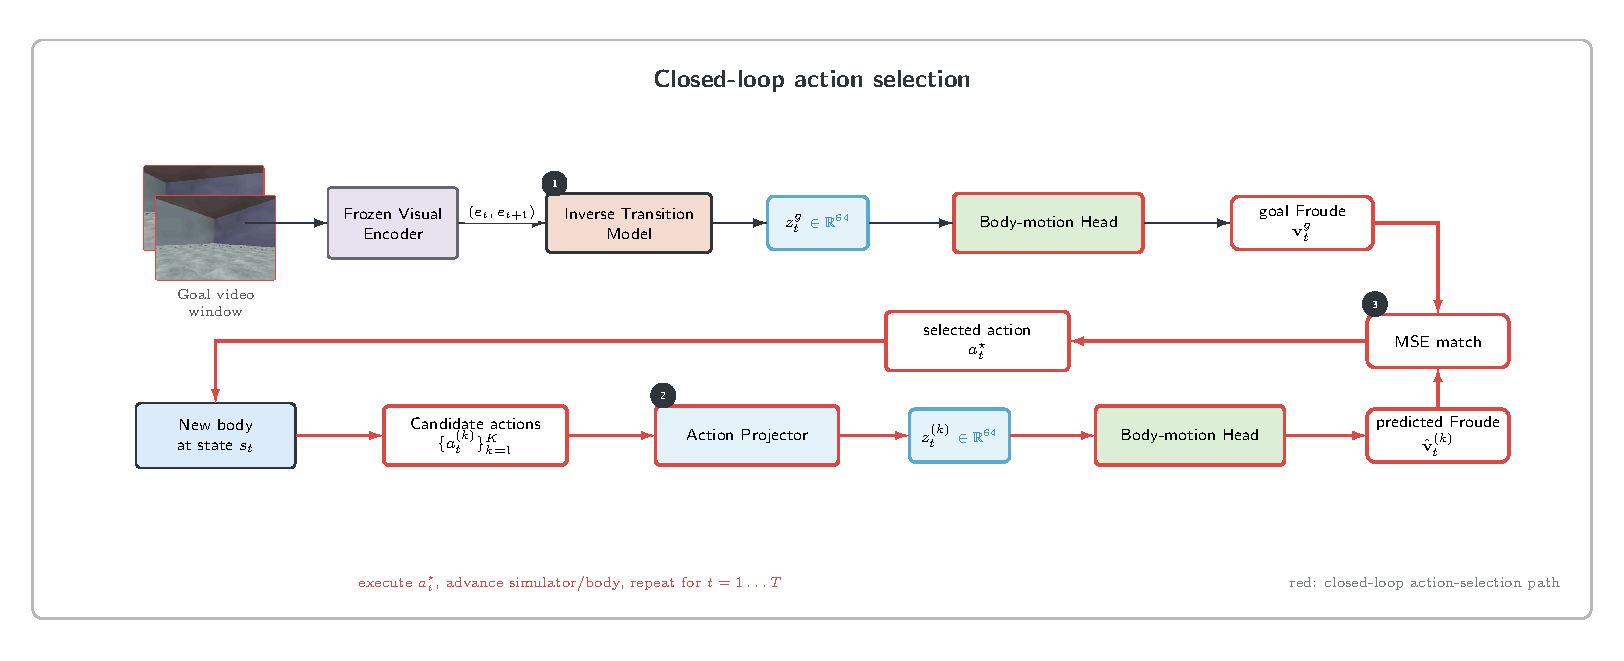
\includegraphics[width=0.85\textwidth]{image/closed_loop_flow.pdf}
\caption{The closed loop this stage tests: a goal read from video is scored against candidate actions, and the best
match is selected. The candidates are recorded actions, so nothing here invents a motion.}
\end{figure}

\noindent The test crosses 2 ways of producing the goal (from the recorded number, physics, or from the source video, vision) with 2 ways of scoring a candidate (directly from its action, or through a rollout of the Forward Transition Model). They are separated on purpose, since bundling them confounded an earlier version of this test.

\subsection{Experiment 3.4: Goal Source and Scoring Mechanism (2$\times$2 Comparison)}


\textbf{Assumption:} candidate scoring can fail on either axis independently, the goal's source (vision versus privileged) or the scoring mechanism (direct versus rollout), and the 2 must be crossed, not bundled, or a failure cannot be attributed.


\textbf{Input:} Goal (vision/physics) $\times$ scoring (direct/rollout).

\textbf{Output:} Selection accuracy, distance to the true goal.


\textbf{Answers:} \textbf{Objectives 2 and 3 together}: transfer quality, and where the closed loop breaks.

\begin{figure}[H]
\centering
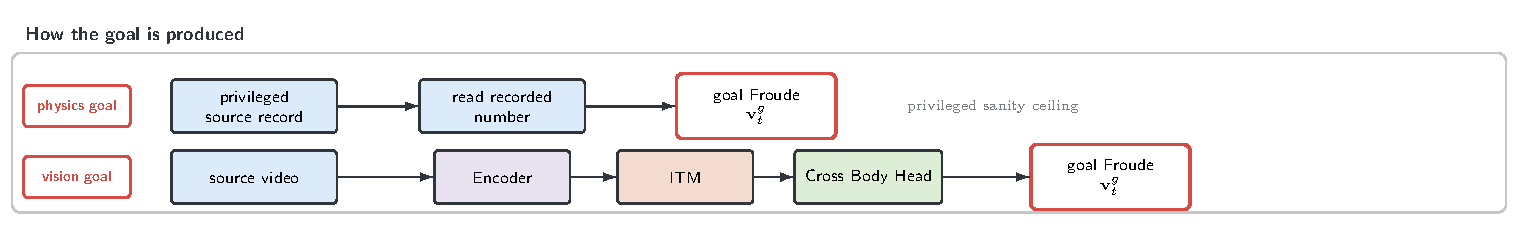
\includegraphics[width=0.75\textwidth]{image/goal_source.pdf}
\caption{How the goal is produced: physics reads the recorded number off the source clip; vision reads it from the clip's video through the Inverse Transition Model and the Cross-Body Head.}
\end{figure}

\begin{figure}[H]
\centering
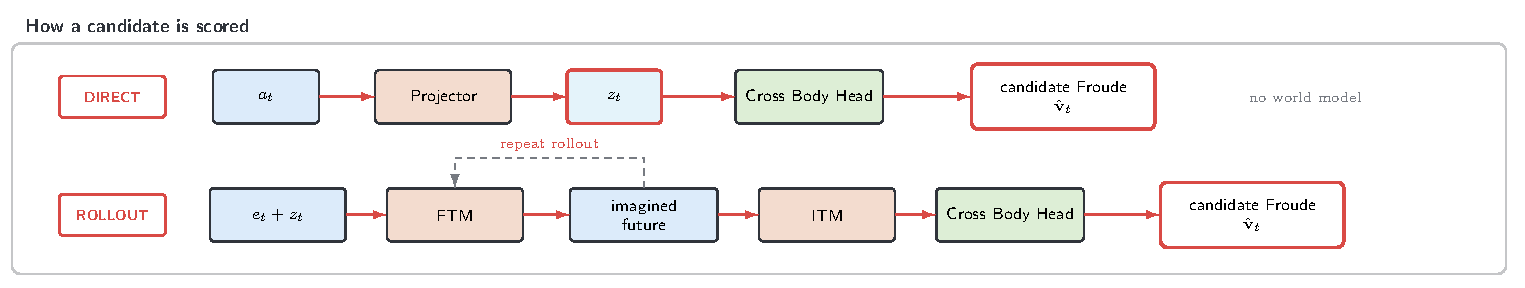
\includegraphics[width=0.75\textwidth]{image/scoring_mode.pdf}
\caption{How a candidate is scored: directly, from its action through the Action Projector and the Cross-Body Head, or through a rollout of the Forward Transition Model. In both cases the pick is the candidate whose Froude value is closest to the goal.}
\end{figure}





\noindent\textbf{Part A: Ground-truth B1 (expert candidate library)}


All 12 hexapod goal conditions, each tracked continuously (an earlier checkpoint, the nearest one available to the checkpoint first reported):


\begin{center}
\footnotesize
\setlength{\tabcolsep}{3pt}
\begin{tabularx}{\textwidth}{>{\hsize=1.14\hsize}Y>{\hsize=1.48\hsize}Y>{\hsize=0.80\hsize\centering\arraybackslash}Y>{\hsize=0.80\hsize\centering\arraybackslash}Y>{\hsize=0.80\hsize\centering\arraybackslash}Y}
\toprule
\textbf{candidate scoring} & \textbf{goal} & \textbf{goal read err} & \textbf{mean error vs. the goal it was given} & \textbf{mean error vs. the true goal} \\
\midrule
direct & physics (privileged) & 0 & \textbf{0.0495} & 0.0495 \\
\addlinespace[3pt]
direct & vision only & 0.0948 & 0.0438 & 0.0964 \\
\addlinespace[3pt]
rollout & physics (privileged) & 0 & 0.1044 & 0.1044 \\
\addlinespace[3pt]
rollout & vision only & 0.0948 & 0.1216 & 0.1467 \\
\bottomrule
\end{tabularx}
\end{center}

*Real Froude units, mean over 12 conditions (goal read err range 0.047 -- 0.188). ``Goal read err'' = mean

\begin{center}
\footnotesize
\setlength{\tabcolsep}{3pt}
\begin{tabularx}{\textwidth}{*{2}{Y}}
\toprule
\textbf{vision-read goal $-$ physics goal} & \textbf{. The last 2 columns differ only for the vision goal: one grades the picks} \\
\bottomrule
\end{tabularx}
\end{center}
against the goal that was read, the other against the true goal. Rollout keeps its input frame fixed across the trial (no live closed loop), so read its numbers with that caveat.*


\textbf{Direct beats rollout on 12/12 conditions under both goal sources. A goal read from video is not free:} the read goal is 0.095 from the truth, and graded against the true goal the vision-driven picks are 0.0964 (direct) and 0.1467 (rollout), against 0.0495 and 0.1044 with the physics goal.

\noindent Paired over the 12 conditions, direct scoring with the physics goal beats rollout by 0.055 (95\% CI 0.035 to 0.081; sign test $p=0.0005$), and the vision-read goal raises the error of direct scoring by 0.047 (CI 0.028 to 0.071; 12 of 12 conditions). Graded against the true goal, direct scoring beats rollout under the vision goal on 10 of 12 conditions (by 0.050, CI 0.032 to 0.067). Almost all of the extra error comes from reading the goal: across conditions the error of the vision-driven picks tracks the goal read error ($r=0.97$).


\textbf{Win case: the third turn level} (clean-split checkpoint fitted on the expert library, 24 candidates, held-out hexapod goal): direct picks 0.0530 from the goal (library best 0.0265), rollout 0.1490; goal read err 0.0321.




\begin{figure}[H]
\centering
\begin{minipage}[t]{0.44\textwidth}\centering
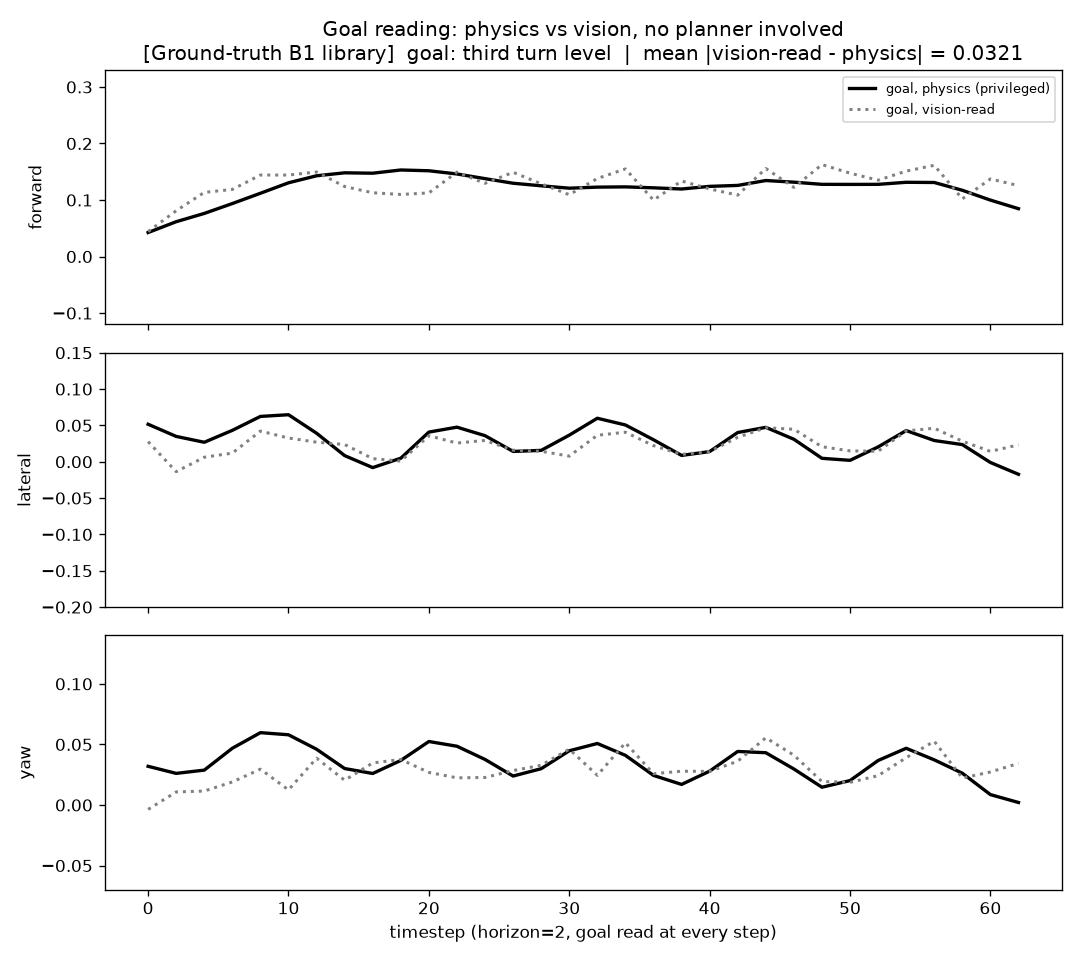
\includegraphics[width=\textwidth]{image/expert_gt_goal_reading_turn_s0.29.png}
\end{minipage}\hfill
\begin{minipage}[t]{0.44\textwidth}\centering
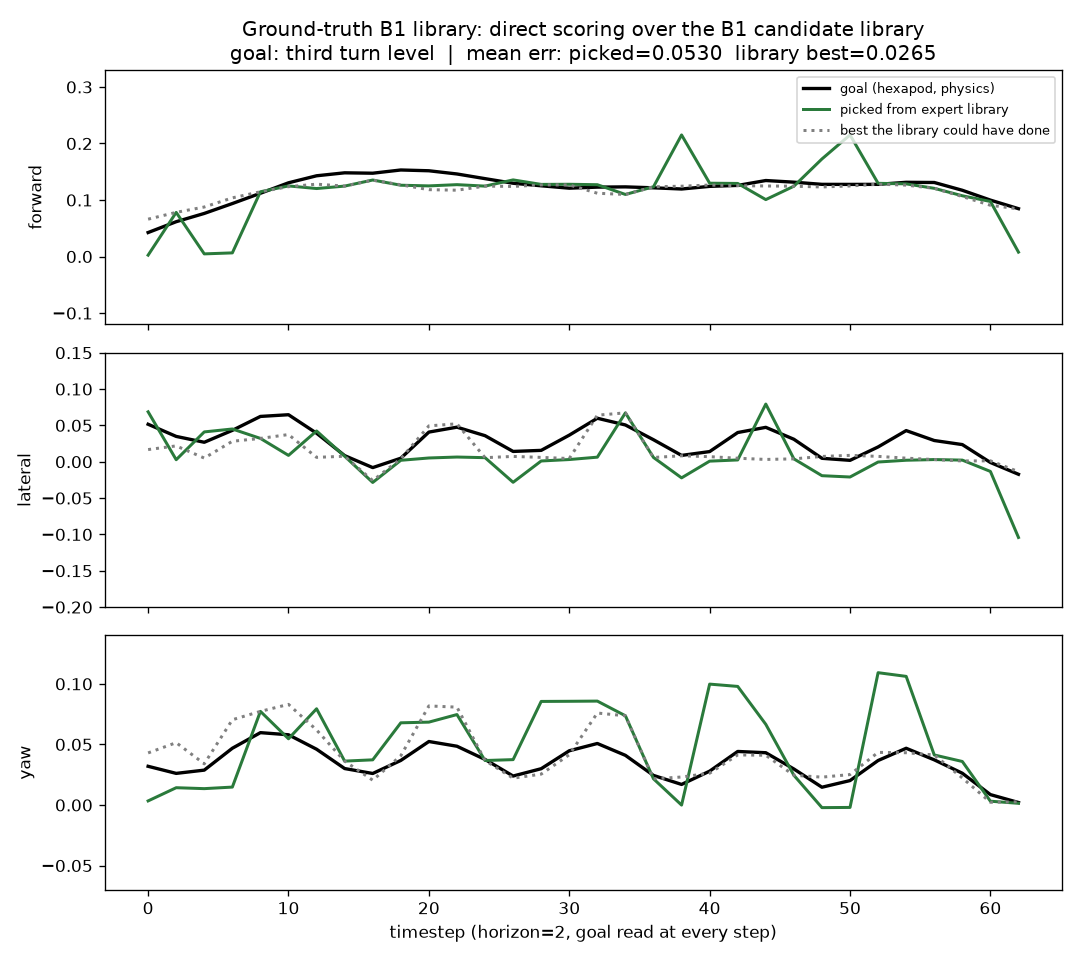
\includegraphics[width=\textwidth]{image/expert_gt_turn_s0.29.png}
\end{minipage}
\caption{Ground-truth B1 library, the third turn level. Left: the goal read from physics and from video. Right: the goal, the pick and the best the library could do, per channel.}
\end{figure}





\begin{figure}[H]
\centering
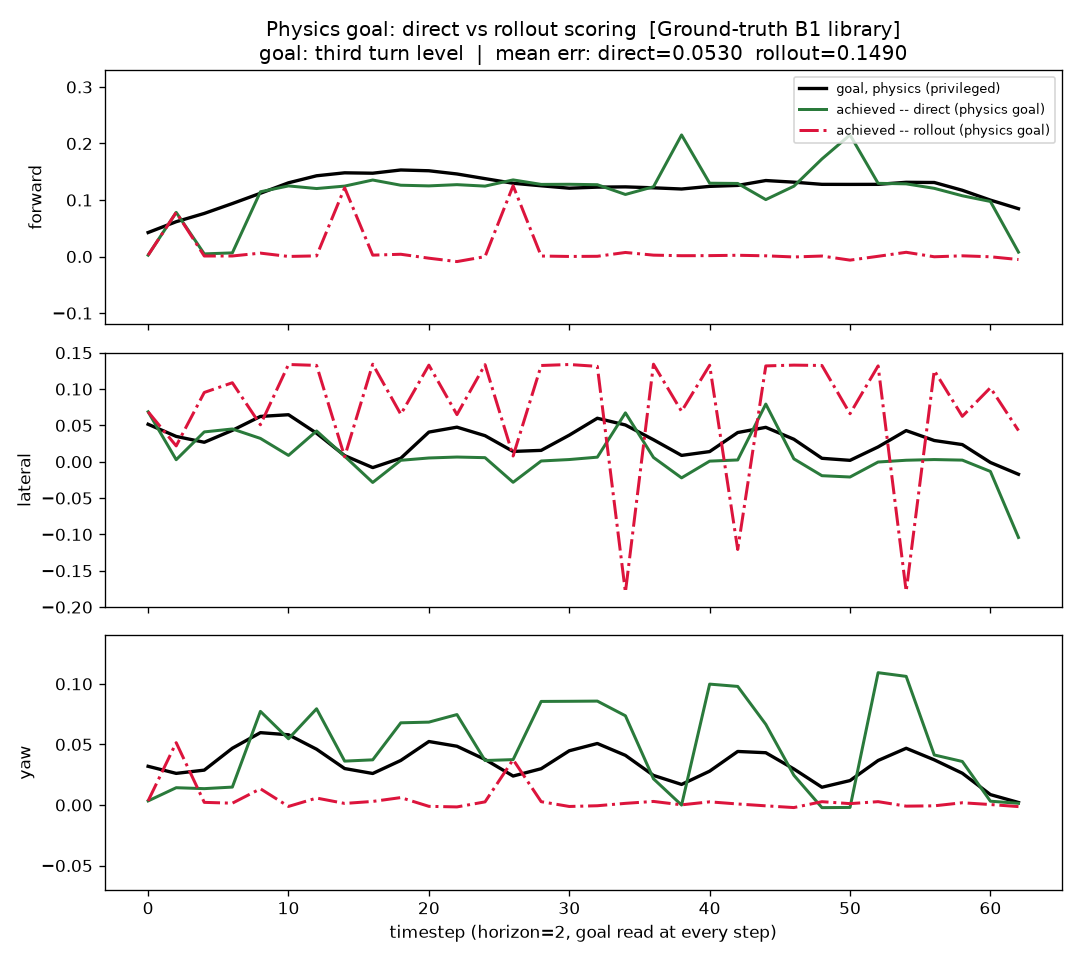
\includegraphics[width=0.44\textwidth]{image/expert_gt_direct_vs_rollout_turn_s0.29.png}
\caption{Ground-truth B1 library, the third turn level: physics goal, direct against rollout scoring.}
\end{figure}


\textbf{Lost case: none.}


\noindent\textbf{Part B: Babble B1 (candidate library from motor babble, no ground-truth B1 clips)}


Steps 1 and 2 fitted on the babble library alone and step 3 on the babble library plus the hexapod clips. Held-out hexapod goals, all 12 conditions, every clip of the library a candidate, real Froude units:


\begin{center}
\footnotesize
\setlength{\tabcolsep}{3pt}
\begin{tabularx}{\textwidth}{>{\hsize=1.72\hsize}Y>{\hsize=0.76\hsize\centering\arraybackslash}Y>{\hsize=0.67\hsize\centering\arraybackslash}Y>{\hsize=0.59\hsize\centering\arraybackslash}Y>{\hsize=1.26\hsize\centering\arraybackslash}Y}
\toprule
\textbf{candidate library} & \textbf{selected} & \textbf{best the library could do} & \textbf{random pick} & \textbf{share of the random-to-best gap recovered} \\
\midrule
expert (24 clips, for reference) & 0.0668 & 0.0315 & 0.121 & 61\% \\
\addlinespace[3pt]
babble v2 (36 clips: forward / sideways / turn) & 0.0923 & 0.0424 & 0.126 & 40\% \\
\addlinespace[3pt]
babble spring (40 clips: forward trot only) & 0.0919 & 0.0725 & 0.110 & 48\% \\
\bottomrule
\end{tabularx}
\end{center}

\noindent The share recovered has 95\% bootstrap intervals over the 12 goals of 49 to 71\% (expert), 31 to 48\% (v2) and 35 to 60\% (spring). All 3 libraries beat a random pick on 12 of 12 goals. The selected error of v2 and spring cannot be told apart (difference $+0.0004$, CI $-0.023$ to $+0.021$); only the gap between the expert library and v2 is distinguishable ($-0.026$, CI $-0.040$ to $-0.011$), and the gap between the expert library and spring is not ($-0.025$, CI $-0.051$ to $-0.003$, Wilcoxon $p=0.13$). Each library was fitted once.

\textbf{Library covers the behavior: the third turn level, babble v2:} picked 0.1002 from the goal, library best 0.0411, random 0.1187; goal read err 0.0400.




\begin{figure}[H]
\centering
\begin{minipage}[t]{0.44\textwidth}\centering
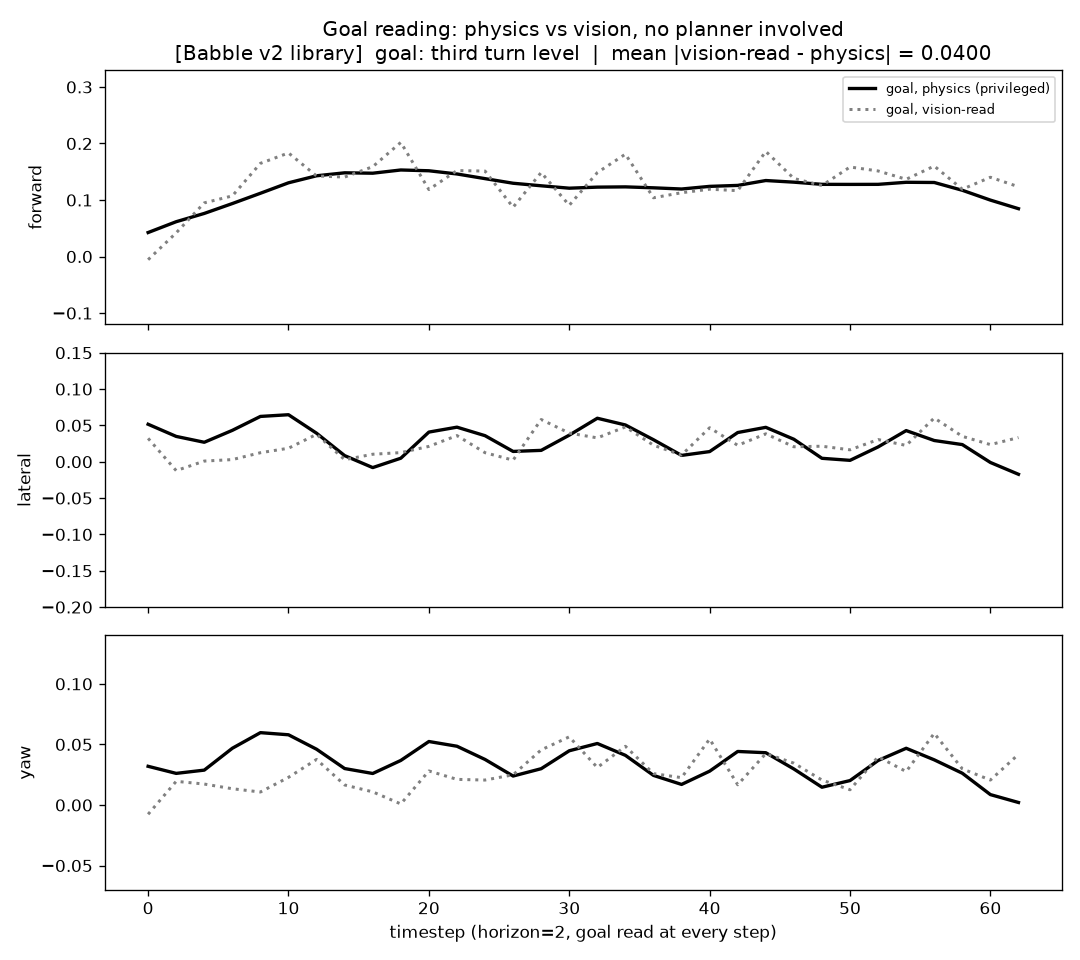
\includegraphics[width=\textwidth]{image/babble_v2_goal_reading_turn_s0.29.png}
\end{minipage}\hfill
\begin{minipage}[t]{0.44\textwidth}\centering
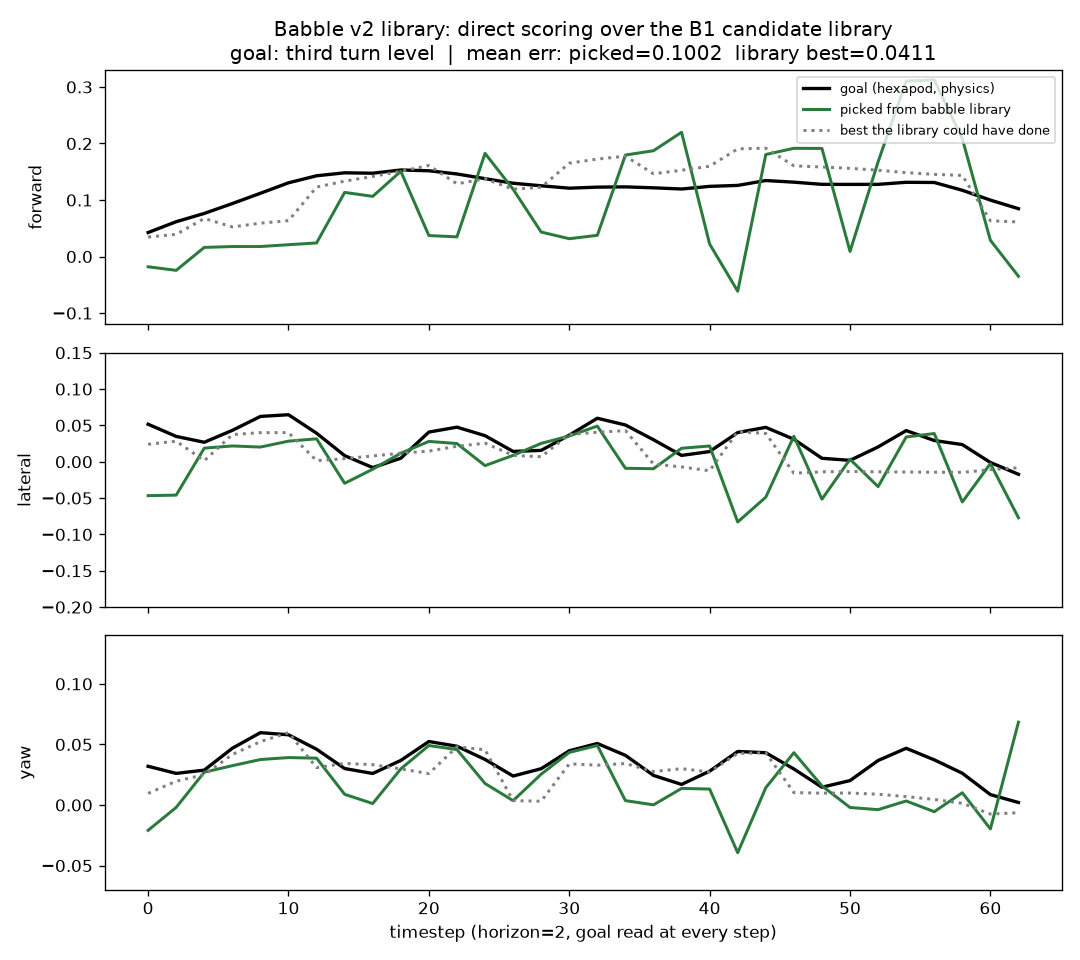
\includegraphics[width=\textwidth]{image/babble_v2_turn_s0.29.png}
\end{minipage}
\caption{Babble v2 library, the third turn level. Left: the goal read from physics and from video. Right: the goal, the pick and the best the library could do, per channel.}
\end{figure}





\textbf{Library lacks the behavior: same goal, the third turn level, babble spring:} the library is forward trot only (clip-mean lateral within $\pm$0.012 and yaw within $\pm$0.018), so its picks cannot follow the goal's lateral and yaw. Picked 0.0717, library best 0.0481, random 0.0885; goal read err 0.0340. Its error is below v2's here because this goal is mostly forward ($\approx$0.13), which spring covers.




\begin{figure}[H]
\centering
\begin{minipage}[t]{0.44\textwidth}\centering
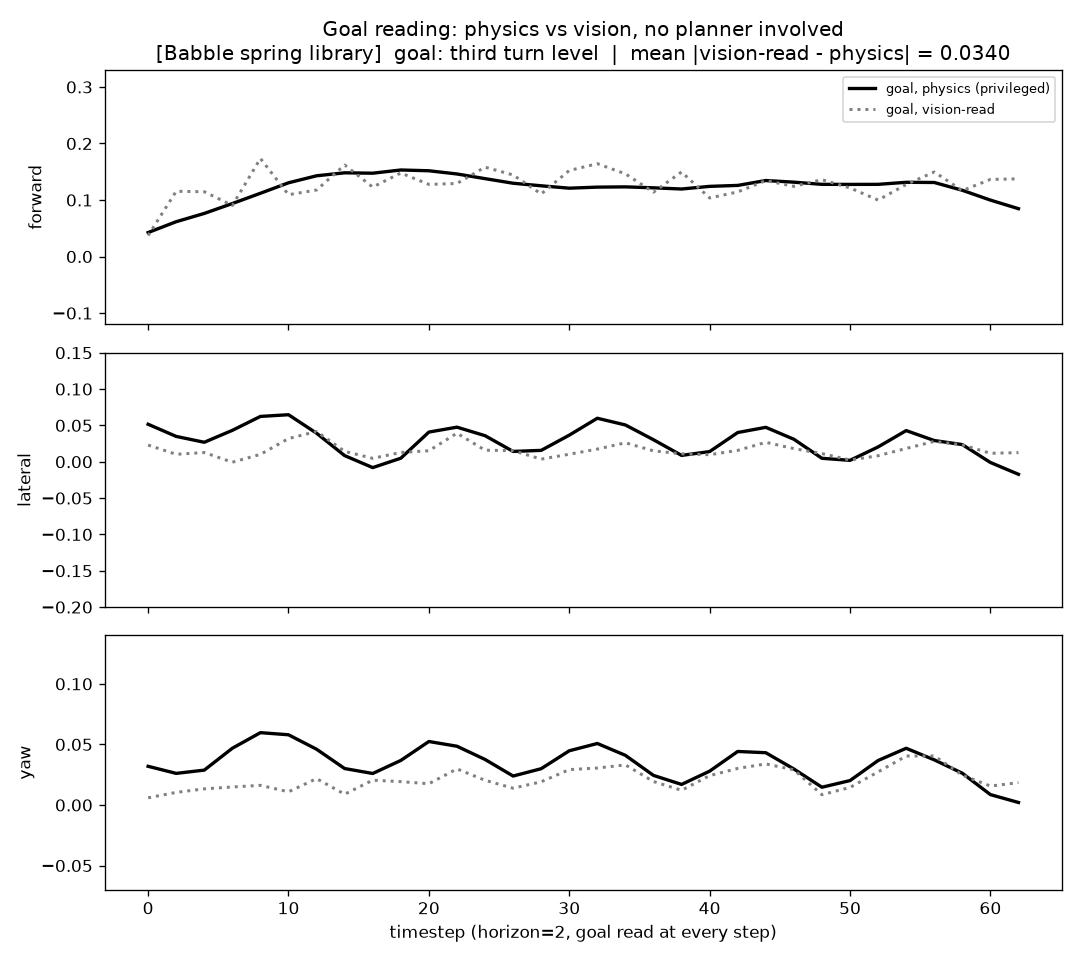
\includegraphics[width=\textwidth]{image/babble_spring_goal_reading_turn_s0.29.png}
\end{minipage}\hfill
\begin{minipage}[t]{0.44\textwidth}\centering
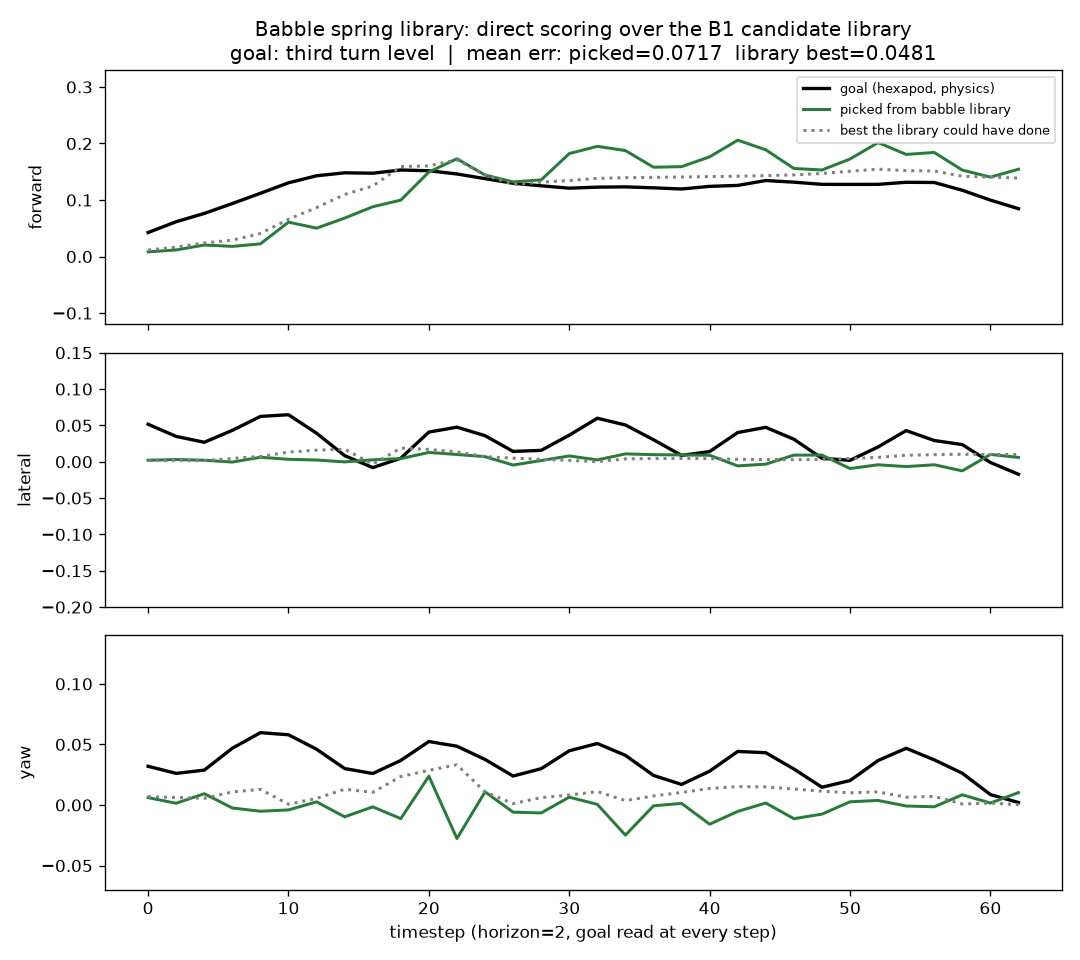
\includegraphics[width=\textwidth]{image/babble_spring_turn_s0.29.png}
\end{minipage}
\caption{Babble spring library, the third turn level. Left: the goal read from physics and from video. Right: the goal, the pick and the best the library could do, per channel.}
\end{figure}





Reminder: these are selections from a library, not a controller. Nothing here can fall; the B1 panels replay recorded clips.


\textbf{Finding:} With the ground-truth B1 library, direct scoring beats rollout on all 12 goal conditions under both goal sources, and a vision-read goal costs accuracy (0.0964 versus 0.0495 against the true goal). With a babble library and no ground-truth B1 clips, direct scoring recovers 40\% (v2) and 48\% (spring) of the random-to-best gap on held-out goals, against 61\% for the expert library.


\textbf{Remaining gap:} 2 different losses: v2 covers the goals (best 0.042) but its scorer loses 0.050 to the best pick, spring's scorer loses 0.019 but the library lacks sideways and turning motion (best 0.114 -- 0.154 on the side goals). Rollout's failure is structural and still unexplained architecturally; bridges to Experiment 3.5.

\subsection{Experiment 3.5: Information Content of the Latent Action $z$}


\textbf{Assumption:} ITM's own transition structure earns its keep over just reading the raw frame pair directly.


\textbf{Input:} $(e_t, e_{t+1})$.

\textbf{Output:} Froude prediction via linear / MLP / $\mathrm{ITM}\to z\to$Cross-Body Head.


\textbf{Answers:} Objective 1: this experiment tests the architecture as well as the objective it is trained under.


\textbf{Result, measured on the real held-out split (the checkpoint used throughout this chapter): the raw frame pair beats the actual pipeline.}


\begin{center}
\footnotesize
\setlength{\tabcolsep}{3pt}
\begin{tabularx}{\textwidth}{>{\hsize=1.89\hsize}Y>{\hsize=0.76\hsize\centering\arraybackslash}Y>{\hsize=0.76\hsize\centering\arraybackslash}Y>{\hsize=0.59\hsize\centering\arraybackslash}Y}
\toprule
\textbf{way to fit Froude} & \textbf{hexapod held-out R$^2$} & \textbf{B1 held-out R$^2$} & \textbf{both pooled} \\
\midrule
linear$(e_t, e_{t+1}) \to$ Froude, no ITM, no $z$ & +0.832 & +0.779 & +0.801 \\
\addlinespace[3pt]
MLP$(e_t, e_{t+1}) \to$ Froude, no ITM, no $z$ & +0.855 & +0.867 & +0.862 \\
\addlinespace[3pt]
\textbf{ITM$(e_t, e_{t+1}) \to z \to$ Cross-Body Head $\to$ Froude (the actual pipeline)} & +0.650 & +0.302 & +0.446 \\
\bottomrule
\end{tabularx}
\end{center}

A function that never touches $z$ at all generalizes clearly better than the pipeline that does. Isolating the input (fitting the same linear/MLP baselines on $z$ itself instead of the raw pair) shows this is not the Cross-Body Head's fit being weak: given the same compressed input, the Cross-Body Head is on par with a fresh head (+0.44--0.47 either way). The information loss is specifically in $z$'s compression, not in how it is read afterward.


Second measurement, same story: cross-embodiment same-behavior clustering in the Cross-Body Head's Froude output, 3-fold held-out.


\begin{center}
\footnotesize
\setlength{\tabcolsep}{3pt}
\begin{tabularx}{\textwidth}{>{\hsize=1.16\hsize}Y>{\hsize=1.18\hsize\centering\arraybackslash}Y>{\hsize=1.24\hsize\centering\arraybackslash}Y>{\hsize=0.41\hsize\centering\arraybackslash}Y}
\toprule
\textbf{representation} & \textbf{cross-embodiment gap} & \textbf{within-embodiment gap} & \textbf{ratio} \\
\midrule
raw z (64-D) & 0.184 & 0.224 & 82\% \\
\addlinespace[3pt]
Cross-Body Head hidden layer (128-D) & 0.065 & 0.109 & 60\% \\
\addlinespace[3pt]
Cross-Body Head Froude output (3-D) & 0.231 & 0.684 & 34\% \\
\bottomrule
\end{tabularx}
\end{center}

The held-out (train-on-2-seeds, test-on-the-3rd) version of this check gives one positive fold and 2 near zero; a much weaker, noisier signal than a clean geometric clustering claim needs.


\textbf{Reading.} This experiment set out to show $z$ itself is the shared cross-embodiment coordinate. It does not hold up: $z$'s compression throws away information the raw frame pair still has, on both tests. That is the same bottleneck the context-collapse fix (Experiment 2.3) targeted: the fix made $z$ sensitive to the action it should use (the action-lever result of Experiment 2.1a), but it did not make $z$ a richer or more clustered representation than the pixels it was built from. The shared coordinate this project has evidence for is Froude itself, read out through the Cross-Body Head, not $z$ as a general-purpose shared latent.

\section{Summary of Results}
\begin{center}
\footnotesize
\setlength{\tabcolsep}{3pt}
\begin{tabularx}{\textwidth}{>{\hsize=0.61\hsize}Y>{\hsize=1.39\hsize}Y}
\toprule
\textbf{Experiment} & \textbf{Finding}\\
\midrule
1.1 Decoder reads the frame? & The decoder was recalling the nearest training body; the cross-body loss term fixes it (command error 3.67$^\circ \to$ 3.44$^\circ$; the image's worth to the decoder 0.4$\times \to$ 9.6$\times$), in distribution.\\
\addlinespace[3pt]
1.2 Inside vs. outside the span & Transfer holds inside the training geometry's span and fails outside it (13.4$^\circ$, $R^2=-0.34$); the failure is predictable in advance from the probe.\\
\addlinespace[3pt]
1.3 Transition vs. pose & One frame reads gait phase almost as well as a frame pair (0.815 vs. 0.840); the gait is periodic ($\approx$6.6 frames); the real action changes prediction error by only 3--9\% at every horizon from 1 to 16 frames.\\
\addlinespace[3pt]
2.1a Shared-coordinate loss & Without the Cross-Body Head term cross-robot readout is negative; with it both directions are positive.\\
\addlinespace[3pt]
2.2 3-step adaptation & B1 goes from failing (ratio 1.061) to real signal on every channel (ratio 0.730, median $\rho$ +0.474); about 12 B1 clips do most of what 24 do.\\
\addlinespace[3pt]
2.4 Camera & An egocentric camera cuts single-frame command recoverability from 0.78 to 0.29, the turn channel of the shared coordinate on the unrefitted B1 goes from 0.07 to 0.64, and $\mathrm{null}/\mathrm{real}$ rises from 1.03; ranking similar actions is not fixed (47\%).\\
\addlinespace[3pt]
2.3 Context collapse & Adding the hinge, readout and 2-step rollout terms keeps $\mathrm{null}/\mathrm{real}$ at 1.06--1.12 at every lag on the combined checkpoint.\\
\addlinespace[3pt]
3.1 Imagination-RL & Converges on one fixed start and goal (return $-15.4 \to -2.7$ under the model's own Froude reading); not shown to generalize across tasks or to hold in physics.\\
\addlinespace[3pt]
3.3 Scoring space & Froude-space scoring turns selection on (76--86\% on the same robot against 18--23\% for frame distance); ranking near-identical actions stays near chance.\\
\addlinespace[3pt]
3.4 The 2$\times$2 & Direct scoring beats rollout scoring on 12/12 goal conditions; a vision-read goal costs accuracy (0.0964 vs. 0.0495 against the true goal); babble libraries recover 40\% and 48\% of the random-to-best gap, against 61\% for the ground-truth B1 library.\\
\addlinespace[3pt]
3.5 Bottleneck & $z$ is a lossy bottleneck; the shared coordinate this project has evidence for is the Froude reading, not $z$.\\
\bottomrule
\end{tabularx}
\end{center}

What remains open is stated in Chapter 5.

\chapter{CONCLUSION AND RECOMMENDATIONS}

\section{Summary of Findings}
This thesis set out to test whether a behavior recorded on one legged robot can be used to select behavior on a
structurally different one from video alone, with no kinematic model, no URDF and no ground-truth demonstrations of the
target, and, in pursuing that, to characterize what a video world model conditioned on the resulting action
representation does and does not use it for. Against the 3 objectives of Section 1.2 and the experiments of
Chapter 4:

\noindent\textbf{Objective 1 (a shared coordinate with no privileged information)} is met for the readout, not for
$z$ itself. With the Cross-Body Head term the readout fitted on one body transfers to the other in both directions
(Experiment 2.1a), but $z$ is a lossy bottleneck, and the coordinate that carries the result is the Froude reading
downstream of it (Experiment 3.5).

\noindent\textbf{Objective 2 (correspondence-free transfer)} is met with adaptation, not zero-shot (Experiment 2.2).
A goal read from the hexapod's video then selects B1 behavior with no frame pairing or retargeting. Direct scoring
beats rollout scoring, and a goal read from video costs accuracy against the true goal. Motor-babble libraries
recover part of the random-to-best gap that the ground-truth library recovers, so the limit lies partly in the library
and partly in the scorer (Experiment 3.4).

\noindent\textbf{Objective 3 (what the action-conditioning achieves, and why)} is met for the mechanism and partly for
the capability. Under a third-person camera the forward model's prediction hardly depends on the action, because a gait
is a limit cycle and the visible pose determines the future (Experiments 1.3 and 2.4). An egocentric camera and a
training objective with a separation term, a frozen readout and a 2-step rollout anchor each restore part of it
(Experiments 2.4 and 2.3). Ranking near-identical actions is not restored (Experiments 2.4 and 3.3), and
imagination-RL converges on one fixed start and goal but not across tasks (Experiment 3.1).

\section{Limitations}
The findings above hold at the strength measured, and no further:
\begin{itemize}[label=--]
\item Transfer needs adaptation, and a goal read from video costs accuracy.
\item $z$ is a lossy bottleneck; the shared coordinate is the Froude reading, not $z$.
\item Ranking near-identical actions stays near chance.
\item Rollout scoring keeps its input frame fixed across a trial, so it is not a closed loop.
\item Imagination-RL converges on one fixed start and goal only.
\item Every selection in Chapter 4 is a choice among recorded clips; nothing is controlled in physics.
\end{itemize}

\section{Recommendations for Remaining Work}
Chapter 4 reports what is confirmed and what is not; this section states what remains, as a plan.

\begin{table}[H]
\centering
\small
\caption{Remaining work plan.}
\label{tab:plan}
\begin{tabularx}{\textwidth}{>{\hsize=0.60\hsize}Y>{\hsize=1.93\hsize}Y>{\hsize=0.48\hsize}Y}
\toprule
\textbf{Item} & \textbf{Activity} & \textbf{Priority}\\
\midrule
Main plan & Action selection on a new body, with no ground truth, from a motor-babble behavior library scored in Froude
  space; next, a library that covers all 3 channels & highest\\
\addlinespace[3pt]
Continuing plan & Debug the open items: the forward model's use of the action, ranking near-identical actions,
  imagination-RL beyond 1 (start, goal) pair, the data cost of adapting to a new body, the action-projector path &
  high\\
\addlinespace[3pt]
Plan B & PPO trained with Froude as the reward; the model-only reward must first pass its local-discrimination
  check & medium\\
\addlinespace[3pt]
Analysis and writing & Consolidate Chapters 4--5 for the final thesis & ongoing\\
\bottomrule
\end{tabularx}
\end{table}

\noindent\textbf{Milestones.} Proposal defended 27 July (done); progress update 23 September (this
report); final defense end of November.

% Category colors: pastel fills. A full-strength cell is done/ongoing, a !40 tint is planned.
\definecolor{tlLit}{RGB}{196,208,224}
\definecolor{tlStage}{RGB}{208,192,240}
\definecolor{tlMain}{RGB}{158,190,245}
\definecolor{tlCont}{RGB}{168,222,186}
\definecolor{tlPlanB}{RGB}{250,200,160}
\definecolor{tlMile}{RGB}{242,170,190}

\newcommand{\tlCell}[1]{\cellcolor{#1}}
\newcommand{\tlMileCell}[1]{\cellcolor{tlMile}\scriptsize\textbf{#1}}
\newcolumntype{M}{>{\centering\arraybackslash}p{1.25cm}}
\newcolumntype{N}{>{\centering\arraybackslash}p{0.7cm}}

\newcommand{\tlKey}[1]{\fcolorbox{black!55}{#1}{%
  \rule{0pt}{5pt}\rule{7pt}{0pt}}}

\begin{table}[H]
\centering
\captionsetup{width=\linewidth, justification=centering}
\caption{Project timeline from June to November 2026.}
\label{tab:project-timeline-ours}
\vspace{0.2cm}
\footnotesize
\setlength{\tabcolsep}{1.5pt}
\renewcommand{\arraystretch}{1.6}
\begin{tabular}{|N|p{5.7cm}|*{6}{M|}}
\hline
\rowcolor{black!8}
\textbf{No.} & \textbf{Activity}
 & \textbf{Jun} & \textbf{Jul} & \textbf{Aug} & \textbf{Sep} & \textbf{Oct} & \textbf{Nov} \\
\hline

1 & Literature review and proposal
 & \tlCell{tlLit} & \tlCell{tlLit} & & & & \\
\hline

2 & Stage 1: pipeline and shared latent objective on the hexapod
 & & & \tlCell{tlStage} & & & \\
\hline

3 & Stage 2: cross-embodiment (hexapod and B1), shared Froude coordinate,
    staged adaptation
 & & & \tlCell{tlStage} & \tlCell{tlStage} & & \\
\hline

4 & Stage 3: closed-loop action selection and imagination-RL
 & & & \tlCell{tlStage} & \tlCell{tlStage} & & \\
\hline

5 & \textbf{Main plan.} Action selection on a new body from a motor-babble
    library, scored in Froude space; then a library covering all 3 channels
 & & & & \tlCell{tlMain} & \tlCell{tlMain!40} & \tlCell{tlMain!40} \\
\hline

6 & \textbf{Continuing plan.} Debug the open items: the forward model's use of
    the action, ranking near-identical actions, imagination-RL beyond 1 goal,
    data cost on a new body
 & & & & \tlCell{tlCont} & \tlCell{tlCont} & \tlCell{tlCont} \\
\hline

7 & \textbf{Plan B.} PPO trained with Froude as the reward
 & & & & \tlCell{tlPlanB!40} & \tlCell{tlPlanB!40} & \tlCell{tlPlanB!40} \\
\hline

8 & \textbf{Milestones}
 & & \tlMileCell{27 Jul} & & \tlMileCell{23 Sep} & & \tlMileCell{end Nov} \\
\hline
\end{tabular}

\vspace{0.45cm}

% Legend
\footnotesize
\begin{tabular}{@{}l@{\hspace{0.4em}}l@{\hspace{1.2em}}l@{\hspace{0.4em}}%
  l@{\hspace{1.2em}}l@{\hspace{0.4em}}l@{}}
\tlKey{tlLit}     & Literature and proposal      &
\tlKey{tlStage}   & Stages 1--3 (done)           &
\tlKey{tlMile}    & Milestone \\[2pt]
\tlKey{tlMain}    & Main plan (first test done)  &
\tlKey{tlMain!40} & Main plan (next)             &
\tlKey{tlCont}    & Continuing plan (ongoing)    \\[2pt]
\tlKey{tlPlanB!40} & Plan B (fallback)           & & & & \\
\end{tabular}

\end{table}

\noindent\textbf{Counterfactual-target training.} A world model trained under teacher forcing can satisfy its
objective without its prediction depending on the action; Section 2.5.1 (UWM-JEPA) proposes counterfactual targets as
the remedy. The limit measured in Section 4.3 is consistent with that pathology. Whether such an objective closes the
gap on a periodic-locomotion domain, where the untrained prediction is already near the achievable ceiling, is
untested and is the most direct next step for the continuing plan.

\noindent\textbf{Candidate separation and scoring circularity.} Scoring among a curated library presupposes a policy
that can already produce the library's behaviors, which is circular for an unseen robot, and no perturbation size
tested was both separable and on-manifold (Section 4.3). The main plan therefore replaces the recorded library with
1 generated by motor babble, in the manner of Hu et al.\ (Section 2.4), plus a library with wider behavioral
coverage rather than larger perturbations of the existing 12. Plan B trains a policy with PPO using the Froude reading
as its reward; forward-only tracking has been reached with a ground-truth reward, and the model-only reward has not
yet shown it can tell a locally better action from a slightly worse one.

\noindent\textbf{Wider coverage is not a free win.} Doubling the library from the 12 matched conditions to 24 (adding
the reverse direction of each: backward speed, the opposite turn sign, and a wider sideways range) was measured
directly, at fixed model capacity, on the same held-out protocol as Section 4.2. The B1's held-out ratio costs
1.24$\times$; the hexapod's costs 2.06$\times$ (0.659 to 0.695 to 1.358 to 3.56 in raw MSE terms once put on the same
units), spreading the same fixed model capacity across twice the behavioral variety. Against that cost, the B1's
forward-channel correlation nearly triples ($\rho$ 0.261 to 0.613), because the wider library is the first source of
real backward-motion signal that body has had. Read together, this is a real, measured trade, not a demonstration
that a wider library is strictly better or strictly worse: covering more behavior costs resolution on each one at a
fixed model size, the same limit the main plan's own library expansion will meet as it widens further.

\section{Closing Statement}
The coordinate that carries the claim of this thesis is a Froude reading downstream of the latent action, not the latent
itself. Transferring it to a structurally different body needs adaptation, and reading the goal from video costs
accuracy. Scoring candidates in that coordinate still selects behavior where scoring in frame space does not. The next
experiment is whether a library generated without any ground-truth clip of the new body is enough to select actions
for it. The first test, on 2 babble libraries, says partly.

% ############################################################################
% #  BACK MATTER                                                              #
% ############################################################################

% ---- References (KMUTT numbered format) ------------------------------------
\begin{thebibliography}{99}
  \addcontentsline{toc}{frontmatter}{REFERENCES}
  \setlength{\itemsep}{4pt}

  \bibitem{hafner2023} D. Hafner, J. Pasukonis, J. Ba, T. Lillicrap, 2023, ``Mastering Diverse Domains through
    World Models (DreamerV3)'', \textbf{arXiv:2301.04104}.
  \bibitem{assran2025} M. Assran, et al., 2025, ``V-JEPA~2: Self-Supervised Video Models Enable Understanding,
    Prediction and Planning'', \textbf{arXiv:2506.09985}.
  \bibitem{huang2026} H. Huang, S. Yenamandra, A. Majumdar, E. Aljalbout, T. Nagarajan, J. Yang, A. Rai,
    M. Rabbat, L. Fei-Fei, J. Wu, T. Wu, F. Meier, 2026, ``Cross-Embodiment Robot Foundation World Models with
    Latent Actions (LAC-WM)'', \textbf{ICML 2026}.
  \bibitem{danesh2026} M. H. Danesh, C. Li, A. Abyaneh, A. Houssaini, K. Ellis, G. Berseth, M. Hutter,
    H.-C. Lin, 2026, ``Toward Hardware-Agnostic Quadrupedal World Models via Morphology Conditioning (QWM)'',
    \textbf{arXiv:2604.08780}.
  \bibitem{li2021} T. Li, R. Calandra, D. Pathak, Y. Tian, F. Meier, A. Rai, 2021, ``Planning in Learned Latent
    Action Spaces for Generalizable Legged Locomotion'', \textbf{IEEE RA-L} (arXiv:2008.11867).
  \bibitem{liang2025} A. Liang, et al., 2025, ``CLAM: Continuous Latent Action Models for Robot Learning from
    Unlabeled Demonstrations'', \textbf{arXiv:2505.04999}.
  \bibitem{larsen2023} A. D. Larsen, T. H. B\"uscher, T. Chuthong, T. Pairam, H. Bethge, S. N. Gorb,
    P. Manoonpong, 2023, ``Self-Organized Stick Insect-Like Locomotion under Decentralized Adaptive Neural
    Control'', \textbf{Advanced Theory and Simulations} 6, 2300228.
  \bibitem{alexander1983} R. McN. Alexander, A. S. Jayes, 1983, ``A dynamic similarity hypothesis for the gaits of
    quadrupedal mammals'', \textbf{Journal of Zoology} 201.
  \bibitem{gupta2022} A. Gupta, et al., 2022, ``MetaMorph: Learning Universal Controllers with Transformers'',
    \textbf{ICLR 2022}.
  \bibitem{zheng2025} Z. Zheng, G. Zhan, B. Shuai, S. Qin, J. Li, T. Zhang, S. E. Li, 2025, ``Transferable
    Latent-to-Latent Locomotion Policy for Efficient and Versatile Motion Control of Diverse Legged Robots (L3P)'',
    \textbf{arXiv:2503.17626}.
  \bibitem{hu2025} Y. Hu, B. Chen, H. Lipson, 2025, ``Egocentric Visual Self-Modeling for Autonomous Robot
    Dynamics Prediction and Adaptation'', \textbf{npj Robotics} (arXiv:2207.03386).
  \bibitem{ahawam2026} J. Cai, L. Ling, S. Chu, et al., 2026, ``AHA-WAM: Asynchronous Horizon-Adaptive
    World-Action Modeling with Observation-Guided Context Routing'', \textbf{arXiv:2606.09811}.
  \bibitem{actswm2026} Z. Gan, Z. Zeng, J. Cheng, Y. Song, Y. Tang, X. Wang, 2026, ``ActSWM: Action-Sensitive
    World Models for Long-Horizon Planning in Open-World Games'', \textbf{arXiv:2607.26712}.
  \bibitem{yeom2026} J. Yeom, H. Kim, J. Park, S. Jung, J. Lee, T. Kim, 2026, ``What Makes Video World Model
    Latents Action-Relevant: Prediction over Reconstruction'', \textbf{arXiv:2606.07687}.
  \bibitem{uwmjepa2026} S. K. Radha, O. Goktas, 2026, ``UWM-JEPA: Predictive World Models That Imagine in
    Belief Space'', \textbf{arXiv:2605.25313}.
  \bibitem{demojepa2026} J. He, G. Li, J. Zhang, C. Hou, Z. Che, S. Zhang, 2026, ``Demo-JEPA:
    Joint-Embedding Predictive Architecture for One-shot Cross-Embodiment Imitation'', \textbf{arXiv:2605.20811}.
  \bibitem{bandura1977} A. Bandura, 1977, ``Social Learning Theory'', \textbf{Prentice-Hall}.
\end{thebibliography}

% ============================================================================
\appendix
\renewcommand{\chaptername}{Appendix}
\chapter{MODEL ARCHITECTURE AND HYPERPARAMETERS}
\addcontentsline{toc}{frontmatter}{APPENDIX}

This appendix gives the full architecture, objective, and hyperparameter specification for the
pipeline described in Chapter 3, at the level of detail Chapter 3 itself summarizes. Values are those
of the current reference checkpoint (the egocentric, hexapod~+~B1 teacher used throughout Chapter 4's
cross-embodiment results); where a field's default in the implementation differs from the value every
reported run trains with, both are given.

\section{Architecture}
Table~\ref{tab:appendix-arch} gives every learned module: what it maps, its shape, and its parameter
count. The encoder is frozen throughout; every other row is trained. 2 modules (LDAD, the
adversary) are architectural options evaluated as ablations and are off in every run this thesis
reports results for. The Stage-2 and Stage-3 checkpoint adds a frozen readout module (a 2-layer MLP, hidden width
512) that carries no learned parameters.

\begin{table}[H]
\centering
\footnotesize
\setlength{\tabcolsep}{4pt}
\caption{Full architecture. Parameter counts are for the reference checkpoint's configuration
(\(z\)-dimension 64, hidden width 512, 16 attention heads throughout).}
\label{tab:appendix-arch}
\begin{tabularx}{\textwidth}{>{\hsize=0.78\hsize}Y>{\hsize=0.98\hsize}Y>{\hsize=1.56\hsize}Y>{\hsize=0.68\hsize}Y}
\toprule
\textbf{Module} & \textbf{Maps} & \textbf{Shape / structure} & \textbf{Parameters}\\
\midrule
Encoder (frozen) & frame $\to$ patch tokens & $256\times256\times3 \to 256\times1408$ &
  $\sim$1B, never updated\\
ITM & $(e_t, e_{t+1}) \to z_t$ & 2 self-attention + 2 cross-attention blocks, hidden 512,
  16 heads $\to z \in \mathbb{R}^{64}$ & 13{,}368{,}384\\
FTM & $(e_t, z_t) \to \hat{e}_{t+1}$ & 8 blocks, hidden 512, 16 heads $\to 256 \times 1408$ &
  77{,}143{,}424\\
Motion Decoder (total) & $(e_t, z_t) \to \hat{a}_t$ & cross-attention backbone,
  $16\times16$ grid pooled $\times2$ & 5{,}499{,}934\\
\quad shared backbone & reads behavior from $z$ vs.\ frame & hidden 512 & 4{,}957{,}184\\
\quad per-embodiment head & latent $\to$ this body's joints & linear, 18-D / 12-D & 272{,}914 /
  269{,}836\\
Cross-body head & $z \to$ body motion, frame-blind, one head for every embodiment &
  LayerNorm $\to 64 \to 128 \to$ \texttt{body\_dim} & 8{,}577\\
Action projector & $a \to z$ (control time, when the ITM's required future frame is unavailable) &
  per-embodiment MLP, depth 2, width 512 & 305{,}216 / 302{,}144\\
LDAD \emph{(ablation, off by default)} & action from $\mathrm{FTM}(e_t,z) - e_t$ & 3 transformer
  layers, 8 heads & --\\
Adversary \emph{(ablation, off by default)} & gradient-reversal body classifier on $z$ &
  hidden 128 & --\\
\bottomrule
\end{tabularx}
\end{table}

The encoder is \texttt{facebook/vjepa2-vitg-fpc64-256} (ViT-g/16). Each frame is encoded
independently through the model's minimal 2-frame tubelet (Section 3.3), so $e_t$ carries no
information from any other timestep.

\section{Pretraining Objective}
The loss trained against for the Stage-2 and Stage-3 checkpoint (the checkpoint behind Experiments 2.2 to 3.5,
\texttt{beh12\_hinge\_\allowbreak cleansplit}) is
\[
\mathcal{L} = 1.0\,\mathcal{L}_{\text{recon}} + 1.0\,\mathcal{L}_{\text{motion}} +
0.5\,\mathcal{L}_{\text{body}} + 0.5\,\mathcal{L}_{\text{hinge}} + 1.0\,\mathcal{L}_{\text{readout}} +
1.0\,\mathcal{L}_{\text{rollout}},
\]
with the hinge horizon $K=2$ and margin $0.1$. The Stage-1 runs (Experiments 1.1 to 1.3) train with
$\lambda_{\text{cross}} = 0.5$ in the \texttt{*\_cross} runs, $\lambda_{\text{body}} = 0$, and none of the hinge,
readout and rollout terms; the zero-weight settings are kept as control arms, isolating what each term contributes, not
as normal practice. Table~\ref{tab:appendix-obj} lists every term the implementation supports, whether it is part of
this weighting, and what each scores.

\begin{table}[H]
\centering
\footnotesize
\setlength{\tabcolsep}{4pt}
\caption{Every loss term the implementation supports. ``Default'' is the implementation's own
starting value; ``In use'' is what the reported runs train with.}
\label{tab:appendix-obj}
\begin{tabularx}{\textwidth}{>{\hsize=0.59\hsize}Y>{\hsize=2.09\hsize}Y>{\hsize=0.63\hsize}Y>{\hsize=0.63\hsize}Y>{\hsize=1.06\hsize}Y}
\toprule
\textbf{Term} & \textbf{Scores} & \textbf{Default} & \textbf{In use} & \textbf{Note}\\
\midrule
recon & $\mathrm{MSE}(\hat{e}_{t+1}, e_{t+1})$ & 1.0 & 1.0 & always on\\
motion & $\mathrm{MSE}(\hat{a}, a)$ through the per-embodiment decoder head & 1.0 & 1.0 & always on\\
body & shared head, $z \to$ body motion, identical head for both robots & 0.0 & \textbf{0.5} & the
  term that carries the cross-embodiment claim (Section 3.4.4)\\
cross & body A's $z$ read against body B's frame, supervised by B's command & 0.0 & 0.0 & 0.5 in the
  Stage-1 leg-length \texttt{*\_cross} runs only\\
adv & gradient-reversal body classifier (loss rising means it is working) & 0.0 & off & ablation\\
hinge & separation between a real- and a null-action rollout over $K$ steps & 0.0 & \textbf{0.5} & Stage 2 and 3
  checkpoint, $K=2$, margin 0.1\\
readout & frozen readout recovering $a$ from the predicted embedding & 0.0 & \textbf{1.0} & Stage 2 and 3
  checkpoint\\
rollout & 2-step auto-regressive consistency, $\mathrm{MSE}(\hat{e}_{t+2}, e_{t+2})$ & 0.0 & \textbf{1.0} & Stage 2 and 3
  checkpoint\\
ldad & action decoded from the predicted state difference & 0.0 & off & ablation\\
\bottomrule
\end{tabularx}
\end{table}

\noindent\textbf{Why $\mathcal{L}_{\text{body}}$ carries the cross-embodiment claim and
$\mathcal{L}_{\text{motion}}$ cannot.} The motion term supervises through \emph{per-embodiment}
decoder heads onto 18- and 12-dimensional joint commands that have no correspondence with each other,
so nothing forces the 2 heads to agree on what $z$ means. The body term uses one head, shared by
both robots, mapping $z$ to body motion alone with no access to the frame: the only term in the
objective that asks the same $z$ to decode the same way on both bodies.

\noindent\textbf{The null action}, used by the ablations above and by the diagnostic comparisons of Chapter 4, is
\[
z_{\text{null}} = \mathrm{ITM}(e_t, e_t),
\]
the latent the model infers when nothing happened between the 2 frames it is shown.

\noindent\textbf{Checkpoint selection} uses
\[
\text{selection} = \lambda_{\text{recon}}\,\mathcal{L}_{\text{recon}} + \lambda_{\text{motion}}\,\mathcal{L}_{\text{motion}}
\]
only, the 2 terms every run has in common, so that a control arm and its matched treatment arm are always
compared at the epoch that minimizes the same quantity. \texttt{total} (which includes whichever experimental
term a given run enables) is never used for this purpose.

\section{Hyperparameters}

\begin{table}[H]
\centering
\footnotesize
\caption{Optimization.}
\label{tab:appendix-opt}
\begin{tabularx}{\textwidth}{YYYY}
\toprule
\textbf{Field} & \textbf{Value} & \textbf{Field} & \textbf{Value}\\
\midrule
Batch size & 8 & Gradient clip & 1.0\\
Learning rate & $1\times10^{-4}$ & Seed & 0\\
Weight decay & 0.01 (AdamW) & Data-loader workers & 4\\
Epochs & 50 & Schedule & cosine, $T_{\max} =$ epochs\\
Precision & fp16 autocast & Device & CUDA (single GPU)\\
\bottomrule
\end{tabularx}
\end{table}

\begin{table}[H]
\centering
\footnotesize
\caption{Model dimensions.}
\label{tab:appendix-dims}
\begin{tabularx}{\textwidth}{YYYY}
\toprule
\textbf{Field} & \textbf{Value} & \textbf{Field} & \textbf{Value}\\
\midrule
Token dimension & 1408 & Latent dimension $z$ & 64\\
Patch grid & $16\times16$ & Hidden width & 512\\
Action dimension & 18 (12 for B1) & Attention heads & 16\\
MLP expansion ratio & 4.0 & Dropout & 0.0\\
ITM self-attn.\ blocks & 2 & FTM blocks & 8\\
ITM cross-attn.\ blocks & 2 & Latent tokens & 1\\
\bottomrule
\end{tabularx}
\end{table}

\begin{table}[H]
\centering
\footnotesize
\setlength{\tabcolsep}{4pt}
\caption{Target construction and timing.}
\label{tab:appendix-time}
\begin{tabularx}{\textwidth}{>{\hsize=0.57\hsize}Y>{\hsize=0.35\hsize}Y>{\hsize=2.08\hsize}Y}
\toprule
\textbf{Field} & \textbf{Value} & \textbf{Meaning}\\
\midrule
\texttt{action\_lag} & 1 & The Motion Decoder is asked for the action that \emph{caused} the
  transition $e_t \to e_{t+1}$, not the action already visible in $e_t$; at lag 0 the target is
  trivially available and $z$ carries nothing (Section 3.6).\\
\texttt{frame\_stride} & 1 & Spacing between the ITM's 2 input frames: one step, 50\,ms at the
  simulator's 20\,Hz.\\
\texttt{action\_chunk} & 0 & Follows \texttt{frame\_stride} automatically, so the reconstruction and
  motion halves of the objective always describe the same time interval.\\
\bottomrule
\end{tabularx}
\end{table}

\begin{table}[H]
\centering
\footnotesize
\setlength{\tabcolsep}{4pt}
\caption{Shared body-motion target (the $\mathcal{L}_{\text{body}}$ term).}
\label{tab:appendix-body}
\begin{tabularx}{\textwidth}{>{\hsize=0.90\hsize}Y>{\hsize=0.51\hsize}Y>{\hsize=0.51\hsize}Y>{\hsize=2.09\hsize}Y}
\toprule
\textbf{Field} & \textbf{Default} & \textbf{In use} & \textbf{Meaning}\\
\midrule
$\lambda_{\text{body}}$ & 0.0 & \textbf{0.5} & weight of the shared-head term\\
\texttt{body\_dim} & 1 & \textbf{3} & must equal the number of channels supervised\\
\texttt{body\_channels} & $(0,)$ & \textbf{$(0,1,2)$} & 0 = forward, 1 = lateral, 2 = yaw\\
\texttt{body\_hidden} & 128 & 128 & width of the shared head\\
\texttt{body\_sees\_frame} & False & False & True reproduces a negative result in which the head
  learns to identify the robot from the frame instead of reading behavior from $z$\\
\bottomrule
\end{tabularx}
\end{table}

\begin{table}[H]
\centering
\footnotesize
\setlength{\tabcolsep}{4pt}
\caption{Data handling and routing.}
\label{tab:appendix-data}
\begin{tabularx}{\textwidth}{>{\hsize=0.98\hsize}Y>{\hsize=0.47\hsize}Y>{\hsize=1.55\hsize}Y}
\toprule
\textbf{Field} & \textbf{Value} & \textbf{Meaning}\\
\midrule
\texttt{within\_body\_std} & True & Motion targets are standardized per body, not pooled across
  bodies (Section 3.5).\\
\texttt{cross\_augment} & True & 2 independently augmented views of every frame pair; the ITM sees
  one, the reconstruction target is drawn from the other (Section 3.4).\\
\texttt{balance\_embodiments} & True & Every embodiment receives an equal share of gradient steps per
  epoch, regardless of how many clips it contributes.\\
\texttt{val\_fraction} / \texttt{heldout\_pairs} & 0.1 / 400 & Validation split size.\\
\texttt{md\_head} / \texttt{md\_pool} & mlp / 2 & Motion Decoder head type and spatial pooling.\\
\texttt{center\_embeddings} & False & Per-embodiment appearance offsets are not subtracted from the
  encoder output before training (kept off).\\
\texttt{ftm\_embodiment\_channel} & False & The FTM is not given the embodiment identity as an extra
  token.\\
\bottomrule
\end{tabularx}
\end{table}

\noindent\textbf{Ablation-specific settings}, active only when the corresponding term in
Table~\ref{tab:appendix-obj} is switched on: hinge margin 0.1 and hinge horizon $K=2$ (both smaller
than the values reported for the source method and than the implementation's default $K=3$, chosen because a wider
margin was found to collapse the term and the hinge horizon is set to the 2 steps the rollout term anchors);
readout-head width 512; LDAD decoder depth 3; adversary hidden width 128 with a 5-epoch warm-up
ramping the reversal strength from 0 to 1.


\section{Implementation Identifiers}
The body of the thesis describes datasets, checkpoints and settings by what they are. Table~\ref{tab:appendix-ids} gives
the identifiers used in the implementation and in the released files.

\begin{table}[H]
\centering
\footnotesize
\setlength{\tabcolsep}{4pt}
\caption{Identifiers used in the implementation, by the description used in the thesis.}
\label{tab:appendix-ids}
\begin{tabularx}{\textwidth}{>{\hsize=0.70\hsize}Y>{\hsize=1.30\hsize}Y}
\toprule
\textbf{Described in the thesis as} & \textbf{Identifier}\\
\midrule
Stage 1 dataset, 9 hexapod bodies & \texttt{fwd\_hex8body}\\
\addlinespace[3pt]
Held-out bodies, scales (0.8, 0.9, 0.9) and (0.6, 0.6, 0.6) & \texttt{c08f09t09}, \texttt{c06f06t06}\\
\addlinespace[3pt]
Nominal hexapod body, scales (1.0, 1.0, 1.0) & \texttt{c10f10t10}\\
\addlinespace[3pt]
Held-out body of the training-diversity comparison & \texttt{c10f10t08}\\
\addlinespace[3pt]
Logged expert foot-trajectory dataset (Larsen et al., 2023) & \texttt{expert\_66k\_aug3c\_fcontact}\\
\addlinespace[3pt]
Lab asset for the stick-insect model & \texttt{airl-insect-walking}\\
\addlinespace[3pt]
Stage 2 dataset, hexapod and B1 & \texttt{beh12}\\
\addlinespace[3pt]
Third turn level, hexapod and B1 & \texttt{turn\_s0.29}, \texttt{turn\_w0.037}\\
\addlinespace[3pt]
Fastest speed, hexapod and B1 & \texttt{speed\_c8.8}, \texttt{speed\_vx0.50}\\
\addlinespace[3pt]
Strongest turn, hexapod and B1 & \texttt{turn\_s0.56}, \texttt{turn\_w0.075}\\
\addlinespace[3pt]
Strong left-sideways level, hexapod and B1 & \texttt{side\_L\_lvl1}\\
\addlinespace[3pt]
Frozen visual encoder & \texttt{facebook/vjepa2-vitg-fpc64-256}\\
\addlinespace[3pt]
Stage 2 and Stage 3 checkpoint & \texttt{beh12\_hinge\_cleansplit}\\
\addlinespace[3pt]
Earlier checkpoint used for the 2$\times$2 table of Experiment 3.4 & \texttt{beh12\_hex-b1\_body3/stage3\_b1\_nce\_s0}\\
\addlinespace[3pt]
Hinge, readout and rollout weights; hinge horizon and margin & \texttt{lambda\_hinge}, \texttt{lambda\_readout}, \texttt{lambda\_rollout}, \texttt{hinge\_K}, \texttt{hinge\_margin}\\
\addlinespace[3pt]
Cross-Body Head; Action Projector & \texttt{body\_head}; \texttt{proj}\\
\addlinespace[3pt]
Ground-truth B1 library (24 clips) and held-out hexapod goals & \texttt{beh12\_b1\_ego\_flat\_cleantrain}, \texttt{beh12\_c10f10t10\_ego\_flat\_cleanheldout}\\
\addlinespace[3pt]
Babble v2 and babble spring libraries & \texttt{b1\_babble\_v2\_ego\_flat}, \texttt{b1\_babble\_coppelia\_spring\_ego\_flat}\\
\bottomrule
\end{tabularx}
\end{table}

\end{document}
